\documentclass[a4paper,12pt]{article}

\usepackage{amsmath,graphicx,fullpage,microtype,hyperref,subfig,hypcap,amsfonts,parskip,pdflscape,multirow,bookmark,titlesec}
%\usepackage{showframe}

\titlespacing\section{0pt}{20pt plus 4pt minus 2pt}{2pt plus 4pt minus 2pt}
\titlespacing\subsection{0pt}{16pt plus 4pt minus 2pt}{2pt plus 4pt minus 2pt}

\widowpenalty=10000
\clubpenalty=10000
\hyphenpenalty=10000
\interfootnotelinepenalty=1000
\DisableLigatures{encoding=*,family=*}
\numberwithin{equation}{section}
\hypersetup{colorlinks,citecolor=black,filecolor=black,linkcolor=black,urlcolor=black}

\renewcommand*{\arraystretch}{1.4}

\begin{document}

\label{sec:Cover Page}
%\addcontentsline{toc}{section}{Cover Page}
\pdfbookmark{Cover Page}{Cover Page}
\thispagestyle{empty}

\href{http://www.bogaardtresearch.tk}{Laurens Bogaardt} \hfill \href{http://www.cam.ac.uk}{University of Cambridge}\\
\href{mailto:lb591@cam.ac.uk}{lb591@cam.ac.uk} \hfill \href{http://www.zoo.cam.ac.uk}{Department of Zoology}\\
\hfill 29-08-2014 \hfill Master's Thesis\\

\vspace{4cm}

\begin{center}
\begin{LARGE}
\begin{bf}
The Evolution of Signals and Amplifiers
\end{bf}
\end{LARGE}
\end{center}

\vspace{3.5cm}

\begin{center}
\begin{minipage}[t]{0.8\textwidth}
\begin{bf}
Abstract
\end{bf}
\vspace{.2cm}
\newline
In 1989, Hasson published an article which introduced the concept of an amplifier within animal communication. This display reduces errors in perception of other characteristics for which there is direct selection. Via its benefit to high quality animals, the amplifier can evolve to fixation and it was suggested that direct choice for the amplifier may emerge. This thesis models the evolution of amplifiers, showing that, if the use of an amplifying display is observable, direct choice will indeed evolve. Consequently, low quality animals may be seen to make use of the display as well, even though it amplifies their lower quality. The two modelling frameworks used in this thesis, evolutionary game theory and signal detection theory, also show how amplifiers can lead to preferences for other types of displays, such as handicap signals, and are used to model the dynamics of such displays. Finally, a simple experiment is conducted to test whether a specific pattern functions as an amplifier.
\end{minipage}
\end{center}

\vspace{1cm}

\begin{center}
\begin{minipage}[t]{0.8\textwidth}
\begin{bf}
Acknowledgements
\end{bf}
\vspace{.2cm}
\newline
The author wishes to thank Prof. Dr. Rufus Johnstone for the supervision during the writing of this thesis. The idea to model observable amplifiers, which was a very interesting and enjoyable experience, came from Dr. Johnstone and this thesis would not have been possible without him. The author also wishes to thank the \href{http://www.cultuurfonds.nl}{Prins Bernhard Cultuurfonds} for partially funding this work.
\end{minipage}
\end{center}

\newpage\clearpage


\phantomsection
\label{sec:Contents}
%\addcontentsline{toc}{section}{Contents}
\pdfbookmark{\contentsname}{Contents}
\renewcommand{\contentsname}{Contents\\} 

\tableofcontents

\newpage\clearpage


\addtocontents{toc}{\protect\vspace{-4mm}}
\part{Introduction}
\label{sec:Introduction}
\addtocontents{toc}{\protect\vspace{1mm}}

\newpage\clearpage


\section{Amplification and Concealment}
\label{sec:Introduction/Amplification and Concealment}
\subsection{Original Definition of Amplifiers}
\label{sec:Original Definition of Amplifiers}

Within sexual selection, the evolution of male displays is driven by female mating preferences. The cost that the display confers on male viability is overcompensated for by the increase in the reproductive success of displaying males. In 1989, Hasson presented a population genetic model which showed that male displays can evolve as a consequence of female mating preferences, even though there was no direct choice for those particular displays~\cite{Hasson1989}. This may occur when females initially base their preferences on a cue that is correlated with some quality-characteristic of the male, such as, for example, viability. If a display amplifies the differences between the various males, it can evolve to fixation. Hasson's idea is that such a display, or amplifier, reduces the error in the perception of a cue by females, improving the correlation between the perceived cue and male quality. This will, then, allow high quality males to benefit more from their high quality cue. On the other hand, a low quality male may do better not to amplify his cue at all. He stands to gain by concealing his bad quality.


\subsection{Names for the Displays}
\label{sec:Names for the Displays}

The names Hasson gave to his idea of a display either increasing the perception of quality differences between males or decreasing those differences were `amplifier' and `attenuator'. The names `revealer' and `concealer' might be better choices. An amplifier of a signal does not increase the strength, size or impact of that signal, but merely reduces the error in its perception on the receiving end. It reveals, as opposed to conceals, true quality. This is different again from what we may call a `detector', which is a display that enhances the detectability of a cue, inducing females to pay attention to the cue in the first place. The opposite of a detector is `camouflage'. An amplifier implicitly assumes the display is already detected and is being assessed. It seems that there remains some confusion over these definitions among empiricists~\cite{Gualla2008}. They perceive these concepts with some error. It is the hope that the models of this thesis will `amplify' the differences in the definitions of amplifiers, quality cues and handicap signals.

\newpage


\section{Previous Models}
\label{sec:Introduction/Previous Models}
\subsection{Unconditional Amplification}
\label{sec:Unconditional Amplification}

In his original article, Hasson describes a two-locus, two-allele, haploid model of \linebreak amplifiers~\cite{Hasson1989}. The two loci control the viability of the male, assumed to a be binary component indicating high or low viability, and whether or not it amplifies. Hasson initially assumes that males are able to amplify their quality cue, but do so independent of their quality. He showed that amplifying displays increase mating success of the more viable males and decrease mating success of the less viable males. An unconditional amplifier can evolve if the average benefit to the more viable amplifying males is higher than the average cost to the less viable amplifying males. It follows that the higher the frequency of the preferred, more viable males, the more likely it is that an amplifier evolves to fixation. Although the modelling method in this thesis is different, the same qualitative result is found in section~\ref{sec:Cue Game with Unconditional Amplification/Conditional Payoffs}. 


\subsection{Conditional Amplification}
\label{sec:Conditional Amplification}

Hasson argues that, due to the negative effect on low quality males, selection will favour the evolution of a modifier which reduces the expression of the amplifier in these males~\cite{Hasson1989}. He adds a coefficient to his model which determines the degree of conditional expression of the amplifier in low quality males. When this coefficient has a non-zero value, Hasson shows that the requirements for the fixation of the amplifier will be less restricted by the negative effect of the display on low quality males. For the extreme case in which low quality males do not amplify at all, Hasson shows that the sole requirement for the evolution of the display is that it benefits high quality males. In section~\ref{sec:Cue Game with Unobservable Amplification/Conditional Payoffs}, we model such conditional amplifiers, but we do not fix the conditionality a priori on low quality males and allow the optimal quality-dependent behaviour to evolve. The results are qualitatively the same as those found by Hasson.


\subsection{Observable Amplification}
\label{sec:Observable Amplification}

As mentioned, Hasson showed that the evolution of amplifiers leads to conditions favouring genetic modifiers which decrease the amplifier's expression in the less viable males~\cite{Hasson1989}. In his original article, Hasson goes on to verbally suggests that this conditional expression may cause selection to favour the evolution of female choice based on the amplifying display itself. Due to the direct correlation of the amplifier with the male's quality, the observation of an amplifier provides information about the male. However, Hasson did not model this step. It is the main purpose of this thesis to model the evolution of amplifiers when females have some ability to detect the use of the display.

\newpage


\section{The Dynamics of Amplification}
\label{sec:Introduction/The Dynamics of Amplification}
\subsection{Amplifiers in Sexual Selection}
\label{sec:Amplifiers in Sexual Selection}

Hasson's original article discussed amplifiers in terms of sexual selection. He proposed that an amplifying display would make differences in male quality more obvious to females. Females often base mating decisions on information they obtain about the male's genetic quality, health, foraging ability or other quality-characteristics~\cite{Jennions1997}. A display which correlates with any of these attributes can provide such information. An amplifier can be, for example, a pattern or a colour which improves the female's perception of the display, increasing the amount of information she obtains. Via its benefits to proud males with a high quality, sexual selection can lead to the fixation of such amplifiers.


\subsection{Amplifiers in Other Types of Selection}
\label{sec:Amplifiers in Other Types of Selection}

Female choice is not the only selection mechanism conceivable which may be responsible for the evolution of amplifiers. Amplifiers can emerge in any communication game in which one player wishes to obtain information about another player. Situations other than sexual selection in which animal communication is important are, for example, parent-offspring conflicts, predator-prey interactions or intra-specific rivalry. We will see two of such examples in section~\ref{sec:Cue Game with Unconditional Amplification/Example} and in section~\ref{sec:Signalling Game/Example}. Consequently, there may be driving forces other than female preferences behind the evolution of amplifiers and the observability of the amplifier may be important to predators or rivals as well.


\subsection{Amplifiers in Economics}
\label{sec:Amplifiers in Economics}

\enlargethispage*{10mm}

Due to its importance in communication systems, amplifiers may not even be restricted to the animal kingdom. In economics, too, information plays a vital role. There are more similarities between economics and zoology. For example, the modelling technique we will apply in part~\ref{sec:The Transition to Signalling through Amplification}, game theory, is used in economics too. Game theory is ideal for understanding the interactions between players with different objectives. As will be mentioned in more detail in section~\ref{sec:The Transition to Signalling}, the signalling model was first introduced by Spence as a description of information transfer in markets~\cite{Spence1973}. It was only later discovered as a mechanism in animal behaviour by Zahavi~\cite{Zahavi1975}. Error-prone quality cues, as well, play a role in economics where asymmetric information may lead businesses to invest a lot in obtaining as much information as possible about a particular market or about a rival. As such, it is expected that one can identify the equivalent of an~amplifier~in~economics.

One possible example would be the year-reports businesses produce to give investors an idea of the `health' of their company. A clear and concise style of writing in such reports would amplify the true health of the company, while an elaborate and confusing style of writing may be used as a trick to obscure negative results. Consequently, it can be expected that the style of writing of the year-reports itself says a lot about a company. Another example is of a job seeker. Someone with a full CV provides a lot of information about their experience and abilities. On the other hand, a person with gaps in their CV may be seen to be hiding something, concealing their lack of quality. Some creative insights are needed to further establish the link between amplifiers and economic theory.

\newpage \clearpage


\section{The Format of this Thesis}
\label{sec:Introduction/The Format of this Thesis}
\subsection{The Transition to Signalling through Amplification}
\label{sec:Introduction/The Transition to Signalling through Amplification}

If high quality males amplify their cue, but low quality males do not, there is a direct correlation between the amplifier and quality. Similarly to the cue, this correlation can provide a female with information about the male. It pays females to be able to observe the use of such a conditional amplifier. The main purpose of this thesis is to model amplifiers which are observable to females. Given that females can tell, to some degree, whether a male has amplified its cue, they may evolve a preference for these amplifiers. Three \textit{Mathematica} notebooks accompany this thesis and contains all the calculations.

In part~\ref{sec:The Transition to Signalling through Amplification} of this thesis, we will model observable amplifiers using evolutionary game theory. Although Hasson made verbal suggestions in this direction, the observability of amplifiers has never been modelled~\cite{Hasson1989}. In order to be able to fully understand all aspects of the model, it is useful to start off simple. As such, part~\ref{sec:The Transition to Signalling through Amplification} contains several sections, each with its own model. The first section starts with the most basic communication game. Following sections build on each other, becoming increasingly more complicated. Each section follows the same structure, including a discussion of the assumptions of the model, the best responses and the equilibrium of the game. We end each section with an illustrative example. Well-established empirical examples of amplifiers are hard to come by, even though the concept of amplification is so general that is can be expected that such displays have evolved in many types of animals. It is the hope that the models of this thesis will entice empiricists to search for evidence for the use of amplifiers.

Besides helping us understand all aspects of amplification better, going through the simpler models in the first sections of part~\ref{sec:The Transition to Signalling through Amplification} serves another purpose. By doing so, we are replicating Hasson's model using a different modelling technique. Hasson used a population genetic model, in which linkage disequilibrium played a role. We will use evolutionary game theory to find under what conditions amplifiers evolve. This modelling method is simple, especially considering the fact that, in part~\ref{sec:The Transition to Signalling through Amplification}, we will stick to binary quality levels and binary choices in amplification. Besides the simplicity of game theory, which allows for a clear oversight of the possible behaviours, this modelling technique also provides an easy way to discuss complex strategies. In section~\ref{sec:Cue Game with Observable Amplification}, we will describe a receiver that is capable of combining information from a quality cue and from its assessment of the use of an amplifying display. The mathematics of evolutionary game theory is perfectly capable of solving for such complex strategies to find the optimal behaviour.

Although Hasson's original article describes his ideas in a single model, it really contains three distinct models of amplifiers. In the first sections of this part of the thesis, we will replicate these models and describe them individually. In section~\ref{sec:Cue Game with Unconditional Amplification}, we will describe a model in which an amplifier can evolve which is unconditional on the quality of the animal. In section~\ref{sec:Cue Game with Conditional Amplification}, we will follow Hasson's example by introducing a coefficient for the degree to which an animal can let the amplifier depend on its quality. Finally, we will model the case in which amplification can fully depend on quality. This is done in section~\ref{sec:Cue Game with Unobservable Amplification}. As in Hasson's original article, it is found that, in this case, low quality animals will opt out of amplifying completely.

\newpage

Finally, the choice of the structure of part~\ref{sec:The Transition to Signalling through Amplification} has a third function. By starting off with the most basic communication game and slowly building it up towards a model of observable amplification, we are following the steps that lead to the evolution of female preferences. The idea that amplifiers can help explain the origin of preferences was mentioned throughout Hasson's original article, however, it has never been modelled completely. As explained more carefully in section~\ref{sec:The Transition to Signalling}, observable amplifiers may indeed provide a pathway to female preferences for any particular display such as, for example, handicap signalling.


\subsection{Amplifiers and Signal Detection Theory}
\label{Introduction/Amplifiers and Signal Detection Theory}

In part~\ref{sec:Amplifiers and Signal Detection Theory} of this thesis, we will again look at observable amplifiers. This time, we will use concepts from signal detection theory to model a display which can amplify a quality cue in a continuous manner. We will start with a basic model in section~\ref{sec:Cue Detection Model}, again to build up our intuition. We, then, extend the mathematics of signal detection theory to allow for the perception of multiple messages. The model of observable amplifiers yields similar results to the one of part~\ref{sec:The Transition to Signalling through Amplification}. In the final two sections of part~\ref{sec:Amplifiers and Signal Detection Theory}, we use the same mathematical framework we developed to model the combination of a quality cue with handicap signalling. This leads to the novel conclusion that handicap signalling is more stable when combined with other cues.


\subsection{Patterns as an Example of Amplifiers}
\label{sec:Introduction/Patterns as an Example of Amplifiers}

Finally, in part~\ref{sec:Patterns as an Example of Amplifiers} of this thesis, we conduct a short experiment in which we test the function of a specific pattern as an amplifier. This pattern was possibly the first ever suggestion of the concept of amplification, by Zahavi, and inspired Hasson to develop his idea~\cite{Zahavi1978}. Therefore, it is interesting to check whether this pattern indeed functions as an amplifier.

\newpage\clearpage


\addtocontents{toc}{\protect\vspace{2mm}}
\part{The Transition to Signalling through Amplification}
\label{sec:The Transition to Signalling through Amplification}
\addtocontents{toc}{\protect\vspace{1mm}}

\newpage\clearpage

\section{Introduction}
\label{sec:Part2/Introduction}
\subsection{The Transition to Signalling}
\label{sec:The Transition to Signalling}

The main purpose of this thesis is to model observable amplifiers. A secondary purpose of part~\ref{sec:The Transition to Signalling through Amplification} of this thesis is to suggest an evolutionary pathway for the origin of female preferences. Hasson has suggested in his original article that, if amplifying displays can becomes observable, they will become attractive to females. This thesis provides the first complete model of observable amplifiers, which shows that such displays indeed become attractive to females.

The attractive amplifiers might evolve further under the pressure of sexual selection and lead to a different type of display. Once direct female choice for a display is established, the conditions may lead to a Fisher runaway process or to handicap signalling~\cite{Hasson1990}. Handicap signalling was first described in Spence's signalling model~\cite{Spence1973}. Within biology, it was independently suggested by Zahavi, using verbal arguments, and modelled by Grafen~\cite{Zahavi1975, Zahavi1977, Grafen1990, Grafen1990a}.

Although the concept is a well established theory of conspicuous male display, like the Fisher runaway process, handicap signalling requires female choice for a particular display well before it pays males to produce that display~\cite{Kirkpatrick1982}. High initial frequency of choice is usually explained by pleiotropy or genetic drift~\cite{Kirkpatrick1982, Heisler1984}. These theories relied on restricting assumptions, however, and had difficulties explaining the origin of direct female choice for a male display when there was a cost involved~\cite{Pomiankowski1987}. The modelling of observable amplifiers can provide a pathway to female preferences and can potentially remove the theoretical difficulty of explaining the origin of direct female choice for any type of male display.

Part~\ref{sec:The Transition to Signalling through Amplification} of this thesis serves to model the dynamics of amplifiers when females have the ability to detect the use of the amplifier. We will combine this purpose with a secondary goal, by also explaining the origin of female preferences and handicap signalling. As can be seen in appendix~\ref{sec:Regions for Costly Amplification}, amplifiers can evolve even when there is a, potentially differential, cost associated to them. The final two sections of part~\ref{sec:The Transition to Signalling through Amplification} show how female choice for such a costly display can evolve and can lead to handicap signalling. We will build up a model, one assumption at a time, which illustrates this transition through amplification to a signalling equilibrium.

\newpage\clearpage


\section{Basic Cue Game}
\label{sec:Basic Cue Game}
\subsection{Necessary Assumptions}
\label{sec:Basic Cue Game/Necessary Assumptions}

In order to explore the effect of observable amplification, let us first start with the most basic communication game. This section serves the sole purpose of familiarising ourselves with the mathematics of female choice. As mentioned in section~\ref{sec:Amplifiers in Other Types of Selection}, the evolution of amplifiers need not be driven by sexual selection. Therefore, we will keep the language of the remainder of part~\ref{sec:The Transition to Signalling through Amplification} neutral. We will focus on the interaction between two individuals, a sender and a receiver. These two `players' are drawn at random from a large population. The sender may vary in some characteristic, which we shall call its quality $q$. For simplicity, let there be only two possible levels of quality, $q\in\{H, L\}$, $H$ for \textit{high}, $L$ for \textit{low}. The proportion of senders with high quality is $0<p<1$, whereas the proportion of low quality senders is $1-p$.

The receiver stands to gain by correctly identifying the quality of the sender and by responding appropriately. Let us assume there are two possible responses. If the receiver assigns $G$, for \textit{good}, to a high quality sender, or $B$, for \textit{bad}, to a low quality sender, it obtains a payoff equal to $1$. If it erroneously assigns $G$ to a low quality sender, or $B$ to a high quality one, it obtains a payoff of zero. The sender always stands to gain by eliciting the favourable response $G$ from the receiver. In this case, it gets a payoff equal to $1$. If the response from the receiver is $B$, the sender obtains a payoff of zero.

The receiver, however, cannot assess the sender's quality with complete accuracy. Instead, it must rely on an error-prone cue $q_{R} \in \{H_{R}, L_{R}\}$, which may take two possible values: $H_{R}$ for the perception of a \textit{high quality} sender, $L_{R}$ for the perception of a \textit{low quality} sender. The subscript `R', in this case, denotes that the perception of quality is done by the \textit{receiver}. While the cue typically takes value $H_{R}$ when the sender is of high quality, and $L_{R}$ when the sender is of low quality, the receiver sometimes observes $L_{R}$ for a high quality sender and $H_{R}$ for a low quality one. Let $0<e_{2}<\frac{1}{2}$ be the probability of error in the assessment of quality, so that the receiver perceives a high quality sender as $H_{R}$ with probability $1-e_{2}$ and as $L_{R}$ with probability $e_{2}$. We will assume symmetrical errors and, therefore, the opposite probabilities apply to a cue from a low quality sender. The parameter $e_{2}$ is a measure of how precisely the receiver can evaluate the quality of the sender.

Having assumed the receiver has some ability to detect the quality of the sender, we can now examine what behaviour would be optimal for such a receiver. At this stage, we need not assume the sender itself is aware of its quality.


\subsection{Extensive Form}
\label{sec:Basic Cue Game/Extensive Form}

Figure~\ref{fig:Model 1/Figure 1.pdf} shows the extensive form of this basic cue game. It shows all the steps in our model, starting in the middle where Nature, $N$, makes a random choice between a high quality sender, $H$, with probability $p$ and a low quality sender, $L$, with probability $1-p$. Nature then makes another random choice between the two possible cues the receiver obtains, either $H_{R}$ or $L_{R}$. The dotted lines indicate the receiver's information set. It cannot perfectly assess whether the observation of quality $H_{R}$ or $L_{R}$ comes from a high or low quality sender. Ultimately, the receiver, R, has to make a choice between assigning the sender with `good' or `bad', either $G$ or $B$. Figure~\ref{fig:Model 1/Figure 1.pdf} also shows the payoffs for each of these possible end-points.

\begin{figure}[h]
\begin{center}
\leavevmode
\includegraphics[scale=.6]{"Model 1/Figure 1.pdf}
\caption{Extensive form}
\label{fig:Model 1/Figure 1.pdf}
\end{center}
\end{figure}


\subsection{Strategies and Strategic Dominance}
\label{sec:Basic Cue Game/Strategic Dominance}

The receiver obtains information about the sender by perceiving it to be either high or low quality. It can choose $G$ or $B$ based on its assessment of the sender's quality. This means its strategies specify two actions; the first is employed when the receiver observes $H_{R}$, the second when $L_{R}$ is perceived. In this simple game, the sender cannot amplify its cue yet. It actually has no strategies at all. However, with future models in mind, let us call the current sender's only strategy $K$, for \textit{conceal}.

In general, the payoff that each player obtains depends on the strategy it chooses and on the strategy of the other player. For both players, some strategies will never do better than other strategies, regardless of the other player's actions. This allows us to remove these strictly and weakly dominated strategies from the list of possibilities under consideration. After the removal of these strategies, some other possibilities may, in turn, become dominated, so these, too, can be eliminated from consideration. This iterative process leaves us with only three undominated strategies for the receiver. This procedure will become more important in future sections. Of the four possible strategies for the receiver, the three undominated ones are given in table~\ref{tab:BasicCueGame/StrategiesR}.

\begin{table}[!h]
\begin{center}
\begin{tabular}{c}
\text{K}
\end{tabular}
\end{center}
\caption{Sender's only strategy}
\label{tab:BasicCueGame/StrategiesS}
\end{table}

\begin{table}[!h]
\begin{center}
\begin{tabular}{ccc}
\text{GG} & \text{GB} & \text{BB}
\end{tabular}
\end{center}
\caption{Receiver's remaining strategies}
\label{tab:BasicCueGame/StrategiesR}
\end{table}

Consider the dominated strategy $BG$ of the receiver. This represents a receiver responding with \textit{bad} when it observes the quality of the sender as high, and responding with \textit{good} when it observes a low quality sender. The payoffs of the model are such that the receiver obtains a payoff of zero if it incorrectly identifies the sender's quality. No matter what the values of the parameters of the model, there is always another strategy which gives a higher payoff than $BG$. Therefore, $BG$ is dominated.


\subsection{Conditional Probabilities and Expected Payoffs}
\label{sec:Basic Cue Game/Conditional Payoffs}

We saw that only a subset of all possible strategies for the receiver were undominated. In general, this makes things more simple, as we will only need to take these undominated strategies into account when determining the best responses for each player to each of the other player's strategies. We will, now, need to determine what behaviour is optimal for the receiver. This is done by examining the expected payoffs given some information about the sender. Since the payoffs of our model are always either 1 or zero, these expected payoffs coincide with the conditional probabilities of having encountered either a high or a low quality sender.

Without any prior information, the receiver knows the probability of dealing with a high quality sender is $p$. This probability changes when the receiver gets a chance to examine the sender properly. It will, then, observe a quality cue which partially informs the receiver about the sender's quality. The expected payoff to the receiver when it responds $G$ is equal to the conditional probability that the sender is of high quality. When the receiver responds $B$, the expected payoff is equal to the conditional probability that the sender is of low quality. These values are listed in table~\ref{tab:BasicCueGame/ConditionalPayoffsR}, along with the conditions under which $G$ yields a greater payoff that $B$.

\begin{table}[h]
\begin{center}
\setlength{\tabcolsep}{.45em}
\begin{tabular}{lcccccrcc}
$P_{R}(G|H_{R})$ & $=$ & $\frac{p(1-e_{2})}{p(1-e_{2})+(1-p)(e_{2})}$ & $\stackrel{?}{>}$ & $\frac{(1-p)(e_{2})}{p(1-e_{2})+(1-p)(e_{2})}$ & $=$ & $P_{R}(B|H_{R})$ & for & $e_{2}<p$\\
$P_{R}(G|L_{R})$ & $=$ & $\frac{p(e_{2})}{p(e_{2})+(1-p)(1-e_{2})}$ & $\stackrel{?}{>}$ & $\frac{(1-p)(1-e_{2})}{p(e_{2})+(1-p)(1-e_{2})}$ & $=$ & $P_{R}(B|L_{R})$ & for & $1-e_{2}<p$
\end{tabular}
\end{center}
\caption{Receiver's expected payoffs}
\label{tab:BasicCueGame/ConditionalPayoffsR}
\end{table}


\subsection{Regions within Parameter-space}
\label{sec:Basic Cue Game/Regions}

Table~\ref{tab:BasicCueGame/ConditionalPayoffsR} allows us to find out how the optimal strategies of the players depend on the parameters of the model. It shows that we can identify different regions within parameter-space. The final results of the model depend greatly on the values of the parameters. In order to understand the model fully, and to be able to say anything about the behaviours of the players, we need to explore all possible parameters. This section, therefore, defines the different regions within parameter-space which influence the receiver's behaviour and provides a simple way of referring to these different behaviours throughout the next sections. Luckily, in this model, all of parameter-space can be divided into only three distinct regions.

\vspace{-4mm}

\begin{table}[h]
\begin{center}
\begin{tabular}{cc}
Region 1: & $p<e_{2}<1-e_{2}$\\
Region 2: & $e_{2}<p<1-e_{2}$\\
Region 3: & $e_{2}<1-e_{2}<p$
\end{tabular}
\end{center}
\caption{Regions}
\label{tab:BasicCueGame/RegionsR}
\end{table}

From table~\ref{tab:BasicCueGame/ConditionalPayoffsR}, we know that the receiver will behave differently depending on whether $p$ is larger or smaller than both $e_{2}$ and $1-e_{2}$. We can now determine what the optimal behaviour is for the receiver, its best response, in each of these regions.


\subsection{Best Responses}
\label{sec:Basic Cue Game/Best Response}

When $p$ is small, smaller than the error in perception $e_{2}$, the number of high quality senders is very low. If a receiver perceives a sender to be of high quality, $H_{R}$, it is more likely that this is due to an error in perception than that the sender is truly of high quality. The receiver should, then, always adopt the response appropriate for a low quality sender:~$B$. If $p$ is very high, the opposite argument holds and the receiver should always adopt the response for a high quality sender:~$G$. Only when $e_{2}<p<1-e_{2}$, which we call region 2, should the receiver pay attention to the quality cue and let this information influence its response. These best responses are summarized in table~\ref{tab:BasicCueGame/BestResponseR}.

\vspace{-1mm}

\begin{table}[h]
\begin{center}
\begin{tabular}{cc}
Region 1: & BB\\
Region 2: & GB\\
Region 3: & GG
\end{tabular}
\end{center}
\caption{Receiver's best response}
\label{tab:BasicCueGame/BestResponseR}
\end{table}


\subsection{Equilibria and Information Content}
\label{sec:Basic Cue Game/Equilibria}

The find out what final result is predicted by our model, we need to combine the behaviours of the sender and the receiver. We will assume that animals optimise their payoffs, which will lead them to the Nash equilibrium of the game. An equilibrium occurs when the strategy of the sender is a best response to the strategy of the receiver, while at the same time the receiver's strategy is a best response to the sender's. As this simplest of all communication models has no actively participating sender, i.e. the sender has no choice in its strategy, the equilibrium of the model is solely determined by the best response of the receiver. Table~\ref{tab:BasicCueGame/Equilibria} shows the equilibrium of the model for each of the three possible regions in parameter-space.

\begin{table}[h]
\begin{center}
\begin{tabular}{cc}
Region 1: & (K, BB)\\
Region 2: & (K, GB)\\
Region 3: & (K, GG)
\end{tabular}
\end{center}
\caption{Equilibria}
\label{tab:BasicCueGame/Equilibria}
\end{table}

It is interesting to look at the information content of the cue the receiver obtains about the quality of the sender. This can be done by first examining the probabilities it assigns to the qualities $H$ and $L$ prior to receiving any information. Naturally, these probabilities must be $p$ and $1-p$, respectively. This can then be compared to the conditional probabilities it assigns after perceiving the cue concerning the sender's quality.

The information content is a good proxy for the correlation between the sender's cue and its true quality and for the response-behaviour of the receiver. The information content can be determined using the standard measure for entropy~\cite{Applebaum1996}. Consider a discrete random variable $X$ with values $x_{1}$, $x_{2}$, ..., $x_{n}$ and associated probabilities $p_{1}$, $p_{2}$, ..., $p_{n}$. The entropy of this random variable is given in equation~\ref{eq:BasicCueGame/EntropyNone}.
\begin{equation}
\label{eq:BasicCueGame/EntropyNone}\
H(X) = - \sum_{j=1}^{n} p_{j} \, \text{Log}[p_{j}]
\end{equation}

In our case, it is the quality of the sender we are uncertain about. Given the two probabilities associated with the two possible outcomes, $H$ and $L$, equation~\ref{eq:BasicCueGame/EntropyNone2} gives the value of the entropy prior to observing anything about the sender.
\begin{equation}
\label{eq:BasicCueGame/EntropyNone2}\
H(q) = - p \, \text{Log}[p] - (1-p) \, \text{Log}[1-p]
\end{equation}

The perceived quality of the sender certainly correlates with the true quality of the sender, however, there is a random element to this perception. The perception of quality, itself, is a random variable. Given two correlated random variables $X$ and $Y$, the conditional entropy of $X$ given that $Y = k$, is defined as in equation~\ref{eq:BasicCueGame/EntropyCue}. Here, $p_{k}(j)$ is the conditional probability that $X = j$ given that $Y = k$.
\begin{equation}
\label{eq:BasicCueGame/EntropyCue}\
H_{k}(X) = - \sum_{j=1}^{n} p_{k}(j) \, \text{Log}[p_{k}(j)]
\end{equation}

It, then, follows that the conditional entropy of $X$ given $Y$ is determined by summing over all possible values of $Y$. In our case, we sum over the two possible perceptions of quality.
\begin{equation}
\label{eq:BasicCueGame/EntropyCue2}\
H_{q_{R}}(q) = \sum_{k \in \{H_{R}, L_{R}\}} p_{k} \, H_{k}(q)
\end{equation}

The information that is conveyed by the quality cue is equal to the reduction in the entropy following the quality perception. In general, this is called the mutual information of $X$ and $Y$ and is denoted $I(X,Y) = H(X) - H_{Y}(X)$. For example, for values of $p = 0.50$ and $e_{2} = 0.20$, the entropy prior to perception is $H_{q} = 1.00$ bits and after perception is $H_{q_{R}}(q) = 0.72$ bits. Therefore, for these values, the information content of the sender's quality cue is $I(q, q_{R}) = 0.28$~bits.


\subsection{Predictions and Example}
\label{sec:Basic Cue Game/Example}

The model we just examined predicts that, if there is a display which correlates with, for example, male viability, male health or male foraging abilities, selection will favour a female preference for this display. In field observations, this display should, therefore, correlate with attractiveness. In an experiment in which the display is manipulated, it can also be expected that male attractiveness would change. The concept of a quality cue is well-known in zoology~\cite{Jennions1997}. However, an example in order to illustrate the simple form of communication described by the basic cue game is always useful.

Male house finches, \textit{Carpodacus mexicanus}, have bright feather colourations, ranging from yellow to red. It has been found that these carotenoid-based plumage colourations are an indicator of nutritional condition during moult, possibly caused by differences in foraging ability~\cite{Hill1994}. Field observations indicate males with brighter colourations have a higher rate of feeding visits, i.e. their parental investment is larger. Furthermore, observations also show that brightly coloured males are more likely to survive to the following year~\cite{Hill1991}. These findings suggest males house finches with brighter colourations have a higher viability and overall better genetic quality. This is supported by the positive correlation between the colouration of fathers and sons~\cite{Hill1991}. The feather colour of males, therefore, serves as a quality cue. It is a display which is honest by design. As such, it can be expected that females will find bright colourations attractive. Both field experiments and laboratory experiments confirm that females displayed a significant preference for the most colourful male~\cite{Hill1990, Hill1991}. This example conforms to our model's predicted behaviour for the equilibrium associated with region 2.

\newpage\clearpage


\section{Cue Game with Unconditional Amplification}
\label{sec:Cue Game with Unconditional Amplification}
\subsection{Additional Assumptions}
\label{sec:Cue Game with Unconditional Amplification/Additional Assumptions}

Following the discussion of amplifiers in section~\ref{sec:Introduction/Previous Models}, we build on our basic communication model and add amplification. We start with the assumptions made in section~\ref{sec:Basic Cue Game/Necessary Assumptions} and now add the assumption that the sender has some influence over the accuracy with which the receiver assesses its quality. To be more precise, the sender may choose one of two possible actions: $A$ for \textit{amplify} and $K$ for \textit{conceal}. If the sender amplifies its quality cue, by choosing action $A$, the error in the receiver's assessment of quality reduces to $0<e_{1}<\frac{1}{2}$, where $e_{1}<e_{2}$. If the sender conceals its quality, by choosing action $K$, the error stays equal to $e_{2}$. Amplification, thus, allows the receiver to evaluate the sender's quality more precisely, by ensuring that the perceived cue correlates more strongly with the actual quality of the sender. By contrast, concealment leads to a higher probability of error in the perception of quality. For simplicity, we will assume that amplification and concealment are cost-free. However, as Hasson showed, amplifiers can evolve even when there is a cost associated with them. This is analysed in appendix~\ref{sec:Regions for Costly Amplification}.

Even though the sender has the ability to amplify its quality cue, we will keep the model as simple as possible, for now, and assume that the sender is unaware of its own quality. Consequently, the strategy the sender chooses is independent of quality. This conforms with Hasson's first model, as described in section~\ref{sec:Introduction/Previous Models}. This section serves the purpose of replicating Hasson's model using a different modelling technique, as well as to build up our intuition of the mechanisms behind amplification. The cue game with unconditional amplification reduces to the basic cue game of section~\ref{sec:Basic Cue Game} when $e_{1}=e_{2}$ and the effect of amplification is nullified.


\subsection{Extensive Form}
\label{sec:Cue Game with Unconditional Amplification/Extensive Form}

Figure~\ref{fig:Model 1/Figure 2.pdf} shows the extensive form of this cue game with unconditional amplification. As described in section~\ref{sec:Basic Cue Game/Extensive Form}, it shows all the steps in our model, starting in the middle where Nature makes a random choice between a high quality sender with probability $p$ and a low quality sender with probability $1-p$. The sender now has the choice to either amplify, $A$, or conceal, $K$, its quality. The dotted lines indicate the sender has no information about its own quality. Depending on the sender's action, Nature makes another random choice, with the appropriate probabilities, between the two possible cues the receiver obtains, either $H_{R}$ or $L_{R}$. The dotted lines indicate the receiver's information set. It cannot perfectly assess whether the observed cue $H_{R}$ or $L_{R}$ comes from a high or low quality sender. Ultimately, the receiver has to make a choice between responding to the sender with $G$ or $B$. Figure~\ref{fig:Model 1/Figure 2.pdf} also shows the payoffs for each of these possible end-points.

\begin{figure}[h]
\begin{center}
\leavevmode
\includegraphics[scale=.49]{"Model 1/Figure 2.pdf}
\caption{Extensive form}
\label{fig:Model 1/Figure 2.pdf}
\end{center}
\end{figure}


\subsection{Strategies and Strategic Dominance}
\label{sec:Cue Game with Unconditional Amplification/Strategic Dominance}

The sender has no information about its own quality, so it has to determine whether or not to amplify, $A$ or $K$, based solely on the probabilities $p$ and $1-p$. The receiver obtains information about the sender by perceiving it to be of either high or low quality. It can choose $G$ or $B$ based on its assessment of the sender's quality. This means the receiver's strategies specify two actions; the first is employed when the receiver observes $H_{R}$, the second when $L_{R}$ is perceived.

\vspace{-4mm}

\begin{table}[h]
\begin{center}
\begin{tabular}{cc}
\text{A} & \text{K}
\end{tabular}
\end{center}
\caption{Sender's strategies}
\label{tab:CueGamewithUnconditionalAmplification/StrategiesS}
\end{table}

\vspace{-1mm}

\begin{table}[h]
\begin{center}
\begin{tabular}{ccc}
\text{GG} & \text{GB} & \text{BB}
\end{tabular}
\end{center}
\caption{Receiver's remaining strategies}
\label{tab:CueGamewithUnconditionalAmplification/StrategiesR}
\end{table}

As described in section~\ref{sec:Basic Cue Game/Strategic Dominance}, the payoff that each player obtains depends on the strategy it chooses and on the strategy of the other player. For both players, some strategies will never do better than other strategies, regardless of the other player's actions. This allows us to remove these strictly and weakly dominated strategies from the list of possibilities under consideration. After the removal of these strategies, some other possibilities may, in turn, become dominated, so these, too, can be eliminated from consideration. In this simple amplification game, the sender can amplify its cue, or conceal it. Neither of these two strategies can be removed. However, the iterative process leaves us with only three undominated strategies for the receiver.


\subsection{Conditional Probabilities and Expected Payoffs}
\label{sec:Cue Game with Unconditional Amplification/Conditional Payoffs}

As described in section~\ref{sec:Basic Cue Game/Conditional Payoffs}, we need to determine the expected payoffs for each player's actions to be able to determine their best responses. Without any knowledge of its own quality, the sender can only choose to amplify or not based on the three possible strategies of the receiver and on $p$. Table~\ref{tab:CueGamewithUnconditionalAmplification/ConditionalPayoffsS} lists the expected payoffs to the sender in each of these cases, and specifies the conditions under which $A$ yields a greater payoff than $K$.

\begin{table}[h]
\begin{center}
\begin{tabular}{lcccccrcc}
$P_{S}(A|GG)$ & $=$ & $1$ & $=$ & $1$ & $=$ & $P_{S}(K|GG)$ & \hspace{2mm} for & any value\\
$P_{S}(A|GB)$ & $=$ & \hspace{22mm} & & \hspace{22mm} & $=$ & $P_{S}(K|GB)$ & \hspace{2mm} \multirow{2}{*}{for} & \multirow{2}{*}{$\frac{1}{2}<p$}
\vspace{-1mm}\\
\multicolumn{3}{r}{$p(1-e_{1})+(1-p)(e_{1})$} & $>$ & \multicolumn{3}{l}{$p(1-e_{2})+(1-p)(e_{2})$} & & 
\vspace{1mm}\\
$P_{S}(A|BB)$ & $=$ & $0$ & $=$ & $0$ & $=$ & $P_{S}(K|BB)$ & \hspace{2mm} for & any value
\end{tabular}
\end{center}
\caption{Sender's expected payoffs}
\label{tab:CueGamewithUnconditionalAmplification/ConditionalPayoffsS}
\end{table}

Without any prior information, the receiver knows the probability of dealing with a high quality sender is $p$. This probability changes when the receiver gets a chance to examine the sender properly. It will, then, observe a quality cue which partially informs the receiver about the sender's quality. The expected payoff to the receiver when it responds $G$ is equal to the conditional probability that the sender is of high quality. When the receiver responds $B$, the expected payoff is equal to the conditional probability that the sender is of low quality. These values are listed in table~\ref{tab:CueGamewithUnconditionalAmplification/ConditionalPayoffsR}, along with the conditions under which $G$ yields a greater payoff that $B$.

\begin{table}[h]
\begin{center}
\setlength{\tabcolsep}{.32em}
\begin{tabular}{lccccclcc}
$P_{R}(G|H_{R},A)$ & $=$ & $\frac{p(1-e_{1})}{p(1-e_{1})+(1-p)(e_{1})}$ & $>$ & $\frac{(1-p)(e_{1})}{p(1-e_{1})+(1-p)(e_{1})}$ & $=$ & $P_{R}(B|H_{R},A)$ & for & $e_{1}<p$\\
$P_{R}(G|L_{R},A)$ & $=$ & $\frac{p(e_{1})}{p(e_{1})+(1-p)(1-e_{1})}$ & $>$ & $\frac{(1-p)(1-e_{1})}{p(e_{1})+(1-p)(1-e_{1})}$ & $=$ & $P_{R}(B|L_{R},A)$ & for & $1-e_{1}<p$\\
$P_{R}(G|H_{R},K)$ & $=$ & $\frac{p(1-e_{2})}{p(1-e_{2})+(1-p)(e_{2})}$ & $>$ & $\frac{(1-p)(e_{2})}{p(1-e_{2})+(1-p)(e_{2})}$ & $=$ & $P_{R}(B|H_{R},K)$ & for & $e_{2}<p$\\
$P_{R}(G|L_{R},K)$ & $=$ & $\frac{p(e_{2})}{p(e_{2})+(1-p)(1-e_{2})}$ & $>$ & $\frac{(1-p)(1-e_{2})}{p(e_{2})+(1-p)(1-e_{2})}$ & $=$ & $P_{R}(B|L_{R},K)$ & for & $1-e_{2}<p$
\end{tabular}
\end{center}
\caption{Receiver's expected payoffs}
\label{tab:CueGamewithUnconditionalAmplification/ConditionalPayoffsR}
\end{table}


\subsection{Regions within Parameter-space}
\label{sec:Cue Game with Unconditional Amplification/Regions}

Table~\ref{tab:CueGamewithUnconditionalAmplification/ConditionalPayoffsS} and table~\ref{tab:CueGamewithUnconditionalAmplification/ConditionalPayoffsR} allow us to find out how the optimal strategies of the players depend on the parameters of the model. The behaviour of the sender is influenced only by a single condition; whether $p<\frac{1}{2}$ or $p>\frac{1}{2}$. Dividing parameter-space into these two regions will give us an easy way to describe the predicted outcome of this model. This condition is very similar to the one found by Hasson~\cite{Hasson1989}. In appendix~\ref{sec:Appendix/Cue Game with Unconditional Amplification}, the equivalent condition for costly amplification is found.

\begin{table}[h]
\begin{center}
\begin{tabular}{lc}
Region S1: & $p<\frac{1}{2}$\\
Region S2: & $\frac{1}{2}<p$
\end{tabular}
\end{center}
\caption{Sender's regions}
\label{tab:CueGamewithUnconditionalAmplification/RegionsS}
\end{table}

In section~\ref{sec:Basic Cue Game/Regions}, we saw that the value of $p$ was the main determining factor influencing the behaviour of the receiver. From table~\ref{tab:CueGamewithUnconditionalAmplification/ConditionalPayoffsR}, we know that the receiver will behave differently depending on how the value of $p$ relates to both $e_{1}$ and $e_{2}$. We can now determine what the optimal behaviour for the receiver is, its best response, in each of these regions.

\begin{table}[h]
\begin{center}
\begin{tabular}{lc}
Region R1: & $p<e_{1}<e_{2}<1-e_{2}<1-e_{1}$\\
Region R2: & $e_{1}<p<e_{2}<1-e_{2}<1-e_{1}$\\
Region R3: & $e_{1}<e_{2}<p<1-e_{2}<1-e_{1}$\\
Region R4: & $e_{1}<e_{2}<1-e_{2}<p<1-e_{1}$\\
Region R5: & $e_{1}<e_{2}<1-e_{2}<1-e_{1}<p$
\end{tabular}
\end{center}
\caption{Receiver's regions}
\label{tab:CueGamewithUnconditionalAmplification/RegionsR}
\end{table}


\subsection{Best Responses}
\label{sec:Cue Game with Unconditional Amplification/Best Response}

As described in section~\ref{sec:Introduction/Previous Models}, Hasson found a simple condition for the evolution of amplifiers. He showed that, if amplification is unconditional, the benefit to the high quality senders must outweigh the cost to the low quality senders before the amplifier can evolve to fixation. It is this same condition which is behind the definition of region S1 and S2 following the expected payoffs of table~\ref{tab:CueGamewithUnconditionalAmplification/ConditionalPayoffsS}. If the proportion of high quality senders is high enough, amplification will be beneficial. The best response for the sender, to any of the receiver's strategies, is to amplify when $p>\frac{1}{2}$.

To obtain this result, we make use of the concept of `trembling hands'. When the receiver responds in the same way regardless of the effect of the amplifier, by adopting either strategy $BB$ or $GG$, the choice of the sender has no influence over its final payoff. The sender is neutral between choosing $A$ or $K$. However, assuming the receiver might accidentally play one of its other undominated strategies with a small probability, and thus play $GB$ sometimes, it still benefits the sender more to conform to the best response to $GB$ in these cases too. It seems reasonable to only take the possible undominated strategies into account when applying the principle of the trembling hand, ignoring, in this case, strategy $BG$. The concept of trembling hands is equivalent to assuming there to be a small level of mutation between strategies. A trembling hand perfect equilibrium is a refinement of the Nash equilibrium.

\begin{table}[h]
\begin{center}
\begin{tabular}{lccc}
 & GG & GB & BB\\
Region S1: & K & K & K\\
Region S2: & A & A & A
\end{tabular}
\end{center}
\caption{Sender's best response}
\label{tab:CueGamewithUnconditionalAmplification/BestResponseS}
\end{table}

When $p$ is small, smaller than the error in perception $e_{1}$, the number of high quality senders is very low. If a receiver perceives a sender to be of high quality, $H_{R}$, it is more likely that this is due to an error in perception than that it is truly a high quality sender. As such, the receiver is better off responding like it has met a low quality sender, $B$. If $p$ is very high, the opposite argument holds and the receiver should always adopt the response for a high quality sender, $G$. When the parameters of the model fall in between these two extremes, the best response depends on the strategy of the sender. In case the sender amplifies, the receiver should adopt the $GB$ strategy. These best responses are summarized in table~\ref{tab:CueGamewithUnconditionalAmplification/BestResponseR}.

\begin{table}[h]
\begin{center}
\begin{tabular}{lccc}
 & A & K\\
Region R1: & BB & BB\\
Region R2: & GB & BB\\
Region R3: & GB & GB\\
Region R4: & GB & GG\\
Region R5: & GG & GG
\end{tabular}
\end{center}
\caption{Receiver's best response}
\label{tab:CueGamewithUnconditionalAmplification/BestResponseR}
\end{table}


\subsection{Equilibria and Information Content}
\label{sec:Cue Game with Unconditional Amplification/Equilibria}

Not unlike the equilibria of our first model in section~\ref{sec:Basic Cue Game/Equilibria}, determining the equilibria of this model is fairly trivial. This is because the best response of the sender is independent from the strategy adopted by the receiver. Only in section~\ref{sec:Cue Game with Observable Amplification} will we see truly interesting strategic interactions between the two players. For now, we simply look at the different regions within parameter-space and list the outcomes dictated by the best responses. For some conditions, such as S2xR1, there is no associated region in parameter-space. The overlap between the two regions is zero. This is because the two conditions contradict each other. A simple `x' indicates when this occurs, as seen in table~\ref{tab:CueGamewithUnconditionalAmplification/Equilibria}.

\begin{table}[h]
\begin{center}
\begin{tabular}{lcc}
 & Region S1 & Region S2\\
Region R1: & (K, BB) & x\\
Region R2: & (K, BB) & x\\
Region R3: & (K, GB) & (A, GB)\\
Region R4: & x & (A, GB)\\
Region R5: & x & (A, GG)
\end{tabular}
\end{center}
\caption{Equilibria}
\label{tab:CueGamewithUnconditionalAmplification/Equilibria}
\end{table}

Like in section~\ref{sec:Basic Cue Game/Equilibria}, it is interesting to look at the information content of the cue the receiver obtains about the quality of the sender. The entropy of the system before any information is obtained about the sender is still given by equation~\ref{eq:BasicCueGame/EntropyNone2}. How much information is conveyed by the sender's quality cue depends on its strategy to amplify or conceal. For example, for values of $p = 0.50$, $e_{1} = 0.10$ and $e_{2} = 0.20$, the entropy prior to perception is $H_{q} = 1.00$ bits and after perception, if concealed, is $H_{q_{R}}(q) = 0.72$ bits. Therefore, in this case, the information content of the sender's cue is $I(q, q_{R}) = 0.28$ bits. However, if the sender amplifies its cue, the entropy after perception is $H_{q_{R}}(q) = 0.47$ bits. In this case, the information content is $I(q, q_{R}) = 0.53$ bits.


\subsection{Predictions and Example}
\label{sec:Cue Game with Unconditional Amplification/Example}

The model we just examined predicts that, if an amplifier enhances the perception of an attractive display, there will be a strong correlation between female preference and the display. There should not, however, be any correlation between the amplifier and female preference. If the amplifier is used regardless of the quality of the sender, there should also not be a correlation between male quality and the display. In an experiment where the amplifier is manipulated and reduced, it can be expected that the correlation between attractiveness and the display weakens. However, the overall attractiveness of the manipulated population should not change. In particular, low quality males should become more attractive, while high quality males should be mistaken for low quality ones more often and become less attractive. In order to illustrate the type of amplification described by the cue game with unconditional amplification, let us look at an example.

The evolution of displays is not restricted to sexual selection and amplifiers may evolve in non-sexual selection cases, such as a predator-prey situation. We had already mentioned this in section~\ref{sec:Amplifiers in Other Types of Selection}. It has been suggested that zebra stripes, combined with the movement and proximity of other individuals with the same pattern, might function as an amplifier of the individual's escape potential~\cite{Ljetoff2007}. As a zebra herd is set in motion by predators, stripes may facilitate the assessment of the moving individuals relative to other individuals in the herd, thereby making more clear which one is the odd-one-out. This, obviously, benefits the high quality zebras. It is not hard to imagine that the expression of the striped pattern is not dependent on the quality of the animal. As such, this might be a case of an unconditional amplifier, where zebras are either unaware of their own quality relative to the group, or unable to change their behaviour accordingly. The consequence is that zebras have stripes because the majority benefit from them, $p>\frac{1}{2}$. This example conforms to our model's predicted behaviour for the equilibrium associated with regions S2xR3 and S2xR4. A similarly unconditional amplifying pattern is present in the spider \textit{Plexippus paykulli} and will briefly be discussed in section~\ref{sec:Cue Game with Unobservable Amplification/Example}.

\newpage\clearpage


\section{Cue Game with Conditional Amplification}
\label{sec:Cue Game with Conditional Amplification}
\subsection{Additional Assumptions}
\label{sec:Cue Game with Conditional Amplification/Additional Assumptions}

So far, we have seen two models. In the first, in section~\ref{sec:Basic Cue Game/Necessary Assumptions}, the receiver perceived a cue correlated with the quality of the sender and acted according to the obtained information. In the second model, in section~\ref{sec:Cue Game with Unconditional Amplification/Additional Assumptions}, the sender had the option of amplifying its cue, but had to do so while unaware of its own quality. One of the purposes of examining these simpler models is to follow the steps evolution would take to arrive at an observable amplifier. This provides a pathway to the origin of female preferences for attractive displays, solving the theoretical problems mentioned in section~\ref{sec:The Transition to Signalling}. We now move on to a further evolutionary state and assume the sender is partially aware of its own quality and can choose whether or not to amplify, action $A$ or action $K$, based on this information. For simplicity, we will assume that amplification and concealment are cost-free. However, as Hasson showed, amplifiers can evolve even when there is a cost associated to them. For this model, this is analysed in appendix~\ref{sec:Appendix/Cue Game with Conditional Amplification}.

As mentioned in section~\ref{sec:Introduction/Previous Models}, Hasson added a coefficient to his model which determined the amount of expression of the amplifier in the low quality sender. We will introduce a similar concept to our model, but we do not fix the conditionality a priori on the low quality sender. By allowing any type of strategy, the optimal quality-dependent behaviour will evolve. The results are qualitatively the same as those found by Hasson. In particular, the sender will now perceive an error-prone cue about its own quality which may take two possible values: $H_{S}$ for the perception of \textit{high quality}, $L_{S}$ for the perception of being a \textit{low quality} sender. The subscript `S' refers to the \textit{sender}. While the cue typically takes value $H_{S}$ when the sender is of high quality, and $L_{S}$ when the sender is of low quality, the sender sometimes observes $L_{S}$ when it is of high quality and $H_{S}$ when it is of low quality. Let $0<e_{4}<\frac{1}{2}$ be the probability of error in the assessment of quality, so that the sender perceives high quality as $H_{S}$ with probability $1-e_{4}$ and as $L_{S}$ with probability $e_{4}$. The opposite probabilities apply to a cue from a low quality sender.

The sender can choose to amplify or to conceal conditionally on this information. An alternative interpretation is that the sender, while fully aware of its own quality, is only partially able to influence its own actions and may be partially predetermined to either amplify or conceal. Therefore, the variable $e_{4}$ captures the sender's ability to detect its own quality, its ability to influence its own level of amplification based on this quality, or a combination of the two. This model reduces to the previous model of section~\ref{sec:Cue Game with Unconditional Amplification} when $e_{4} = \frac{1}{2}$ and to the following model of section~\ref{sec:Cue Game with Unobservable Amplification} when $e_{4} = 0$.


\subsection{Extensive Form}
\label{sec:Cue Game with Conditional Amplification/Extensive Form}

Figure~\ref{fig:Model 1/Figure 3.pdf} shows the extensive form of this cue game with conditional amplification. Similar extensive forms were already described in section~\ref{sec:Basic Cue Game/Extensive Form} and in section~\ref{sec:Cue Game with Unconditional Amplification/Extensive Form}. The only addition in this model is the cue the sender receives about its own quality. This information is error-prone, therefore it is Nature which makes a random choice between $H_{S}$ and $L_{S}$, with the appropriate probabilities.

\begin{figure}[h]
\begin{center}
\leavevmode
\includegraphics[scale=.47]{"Model 1/Figure 3.pdf}
\caption{Extensive form}
\label{fig:Model 1/Figure 3.pdf}
\end{center}
\end{figure}


\subsection{Strategies and Strategic Dominance}
\label{sec:Strategic Dominance}

Now that the sender has at least some information about its own quality, it may use this information in its decision to amplify or not. It follows that the sender has strategies specifying two actions: the first to be employed when it believes to be of high quality, the second action to be employed in case of the perception of low quality. The receiver still obtains information about the sender via a quality cue. It chooses $G$ or $B$ based on this assessment and has strategies specifying two actions.

As usual, testing which of these is dominated reduces the list of strategies to consider. Table~\ref{tab:CueGamewithConditionalAmplification/StrategiesS} lists the remaining strategies for the sender, while table~\ref{tab:CueGamewithConditionalAmplification/StrategiesR} shows the receiver's remaining strategies.

\vspace{-3mm}

\begin{table}[!h]
\begin{center}
\begin{tabular}{ccc}
\text{AA} & \text{AK} & \text{KK}
\end{tabular}
\end{center}
\caption{Sender's remaining strategies}
\label{tab:CueGamewithConditionalAmplification/StrategiesS}
\end{table}

\vspace{-2mm}

\begin{table}[!h]
\begin{center}
\begin{tabular}{ccc}
\text{GG} & \text{GB} & \text{BB}
\end{tabular}
\end{center}
\caption{Receiver's remaining strategies}
\label{tab:CueGamewithConditionalAmplification/StrategiesR}
\end{table}


\subsection{Conditional Probabilities and Expected Payoffs}
\label{sec:Cue Game with Conditional Amplification/Conditional Payoffs}

As described in section~\ref{sec:Basic Cue Game/Conditional Payoffs} and in section~\ref{sec:Cue Game with Unconditional Amplification/Conditional Payoffs}, the expected payoffs allow us to define the different regions of parameter-space and the best responses for both players within these regions. Now that the sender has non-trivial strategies, its expected payoff will not only depend on the receiver's choices, but also on the information it obtains about its own quality. Table~\ref{tab:CueGamewithConditionalAmplification/ConditionalPayoffsS} lists these expected payoffs, and specifies the conditions under which $A$ yields a greater payoff than $K$.

\begin{table}[h]
\begin{center}
\begin{tabular}{lcccccrcc}
$P_{S}(A|H_{S},GG)$ & $=$ & $1$ & $=$ & $1$ & $=$ & $P_{S}(K|H_{S},GG)$ & for & any value\\
$P_{S}(A|L_{S},GG)$ & $=$ & $1$ & $=$ & $1$ & $=$ & $P_{S}(K|L_{S},GG)$ & for & any value\\
$P_{S}(A|H_{S},GB)$ & $=$ & \hspace{16mm} & & \hspace{16mm} & $=$ & $P_{S}(K|H_{S},GB)$ & \multirow{2}{*}{for} & \multirow{2}{*}{$e_{4}<p$}
\vspace{-1mm}\\
\multicolumn{3}{r}{$\frac{p(1-e_{4})(1-e_{1})+(1-p)(e_{4})(e_{1})}{p(1-e_{4})+(1-p)(e_{4})}$} & $>$ & \multicolumn{3}{l}{$\frac{p(1-e_{4})(1-e_{2})+(1-p)(e_{4})(e_{2})}{p(1-e_{4})+(1-p)(e_{4})}$} &
\vspace{1mm}\\
$P_{S}(A|L_{S},GB)$ & $=$ & & & & $=$ & $P_{S}(K|L_{S},GB)$ & \multirow{2}{*}{for} & \multirow{2}{*}{$1-e_{4}<p$}
\vspace{-1mm}\\
\multicolumn{3}{r}{$\frac{p(e_{4})(1-e_{1})+(1-p)(1-e_{4})(e_{1})}{p(e_{4})+(1-p)(1-e_{4})}$} & $>$ & \multicolumn{3}{l}{$\frac{p(e_{4})(1-e_{2})+(1-p)(1-e_{4})(e_{2})}{p(e_{4})+(1-p)(1-e_{4})}$} & 
\vspace{1mm}\\
$P_{S}(A|H_{S},BB)$ & $=$ & $0$ & $=$ & $0$ & $=$ & $P_{S}(K|H_{S},BB)$ & for & any value\\
$P_{S}(A|L_{S},BB)$ & $=$ & $0$ & $=$ & $0$ & $=$ & $P_{S}(K|L_{S},BB)$ & for & any value
\end{tabular}
\end{center}
\caption{Sender's expected payoffs}
\label{tab:CueGamewithConditionalAmplification/ConditionalPayoffsS}
\end{table}

Table~\ref{tab:CueGamewithConditionalAmplification/ConditionalPayoffsR} lists the expected payoffs for the receiver as a function of the sender's strategy and the model's parameters, along with the conditions under which $G$ yields a greater payoff that $B$.

\begin{table}[h]
\begin{center}
\setlength{\tabcolsep}{.22em}
\begin{tabular}{lcccccrcc}
$P_{R}(G|H_{R},AA)$ & $=$ & $\frac{p(1-e_{1})}{p(1-e_{1})+(1-p)(e_{1})}$ & $>$ & $\frac{(1-p)(e_{1})}{p(1-e_{1})+(1-p)(e_{1})}$ & $=$ & $P_{R}(B|H_{R},AA)$ & for & $e_{1}<p$\\
$P_{R}(G|L_{R},AA)$ & $=$ & $\frac{p(e_{1})}{p(e_{1})+(1-p)(1-e_{1})}$ & $>$ & $\frac{(1-p)(1-e_{1})}{p(e_{1})+(1-p)(1-e_{1})}$ & $=$ & $P_{R}(B|L_{R},AA)$ & for & $1-e_{1}<p$
\vspace{1mm}\\
$P_{R}(G|H_{R},AK)$ & $=$ & \multicolumn{7}{l}{$\frac{p(1-e_{4})(1-e_{1})+p(e_{4})(1-e_{2})}{p(1-e_{4})(1-e_{1})+p(e_{4})(1-e_{2})+(1-p)(e_{4})(e_{1})+(1-p)(1-e_{4})(e_{2})}$}
\vspace{1mm}\\
\multicolumn{5}{r}{$> \frac{(1-p)(e_{4})(e_{1})+(1-p)(1-e_{4})(e_{2})}{p(1-e_{4})(1-e_{1})+p(e_{4})(1-e_{2})+(1-p)(e_{4})(e_{1})+(1-p)(1-e_{4})(e_{2})}$} & $=$ & $P_{R}(G|H_{R},AK)$ & for & $f_{1}<p$
\vspace{2mm}\\
$P_{R}(G|L_{R},AK)$ & $=$ & \multicolumn{7}{l}{$\frac{p(1-e_{4})(e_{1})+p(e_{4})(e_{2})}{p(1-e_{4})(e_{1})+p(e_{4})(e_{2})+(1-p)(e_{4})(1-e_{1})+(1-p)(1-e_{4})(1-e_{2})}$}
\vspace{1mm}\\
\multicolumn{5}{r}{$> \frac{(1-p)(e_{4})(1-e_{1})+(1-p)(1-e_{4})(1-e_{2})}{p(1-e_{4})(e_{1})+p(e_{4})(e_{2})+(1-p)(e_{4})(1-e_{1})+(1-p)(1-e_{4})(1-e_{2})}$} & $=$ & $P_{R}(G|L_{R},AK)$ & for & $f_{2}<p$
\vspace{2mm}\\
$P_{R}(G|H_{R},KK)$ & $=$ & $\frac{p(1-e_{2})}{p(1-e_{2})+(1-p)(e_{2})}$ & $>$ & $\frac{(1-p)(e_{2})}{p(1-e_{2})+(1-p)(e_{2})}$ & $=$ & $P_{R}(B|H_{R},KK)$ & for & $e_{2}<p$\\
$P_{R}(G|L_{R},KK)$ & $=$ & $\frac{p(e_{2})}{p(e_{2})+(1-p)(1-e_{2})}$ & $>$ & $\frac{(1-p)(1-e_{2})}{p(e_{2})+(1-p)(1-e_{2})}$ & $=$ & $P_{R}(B|L_{R},KK)$ & for & $1-e_{2}<p$
\end{tabular}
\end{center}
\caption{Receiver's expected payoffs}
\label{tab:CueGamewithConditionalAmplification/ConditionalPayoffsR}
\end{table}

In table~\ref{tab:CueGamewithConditionalAmplification/ConditionalPayoffsR}, the conditions which describe the relation between the expected payoffs for both the receiver's perceptions, when the sender plays its $AK$ strategy, result in long expressions. Equation~\ref{eq:f1andf2} gives these expressions.

\begin{subequations}
\label{eq:f1andf2}
\begin{gather}
f_{1}(e_{1},e_{2},e_{4})=\frac{e_{2}-e_{4}(e_{2}-e_{1})}{1+(e_{2}-e_{1})-2 e_{4}(e_{2}-e_{1})}\\
f_{2}(e_{1},e_{2},e_{4})=\frac{1-e_{2}+e_{4}(e_{2}-e_{1})}{1-(e_{2}-e_{1})+2 e_{4}(e_{2}-e_{1})}
\end{gather}
\end{subequations}

Equation~\ref{eq:f1andf2} defines a boundary in parameter-space which separates regions for which the best course of action for the receiver differs.


\subsection{Regions within Parameter-space}
\label{sec:Cue Game with Conditional Amplification/Regions}

The distinct regions of parameter-space which are important to the sender are listed in table~\ref{tab:CueGamewithConditionalAmplification/RegionsS}.

\begin{table}[h]
\begin{center}
\begin{tabular}{lc}
Region S1: & $p<e_{4}<1-e_{4}$\\
Region S2: & $e_{4}<p<1-e_{4}$\\
Region S3: & $e_{4}<1-e_{4}<p$
\end{tabular}
\end{center}
\caption{Sender's regions}
\label{tab:CueGamewithConditionalAmplification/RegionsS}
\end{table}

The regions of parameter-space which are important to the receiver are listed in table~\ref{tab:CueGamewithConditionalAmplification/RegionsR}. It can be checked that $f_{1}$ always lies between $e_{1}$ and $e_{2}$. Likewise, $f_{2}$ always falls in between $1-e_{2}$ and $1-e_{1}$.

\begin{table}[h]
\begin{center}
\begin{tabular}{lc}
Region R1: & $p<e_{1}<f_{1}(e_{1},e_{2},e_{4})<e_{2}<1-e_{2}<f_{2}(e_{1},e_{2},e_{4})<1-e_{1}$\\
Region R2: & $e_{1}<p<f_{1}(e_{1},e_{2},e_{4})<e_{2}<1-e_{2}<f_{2}(e_{1},e_{2},e_{4})<1-e_{1}$\\
Region R3: & $e_{1}<f_{1}(e_{1},e_{2},e_{4})<p<e_{2}<1-e_{2}<f_{2}(e_{1},e_{2},e_{4})<1-e_{1}$\\
Region R4: & $e_{1}<f_{1}(e_{1},e_{2},e_{4})<e_{2}<p<1-e_{2}<f_{2}(e_{1},e_{2},e_{4})<1-e_{1}$\\
Region R5: & $e_{1}<f_{1}(e_{1},e_{2},e_{4})<e_{2}<1-e_{2}<p<f_{2}(e_{1},e_{2},e_{4})<1-e_{1}$\\
Region R6: & $e_{1}<f_{1}(e_{1},e_{2},e_{4})<e_{2}<1-e_{2}<f_{2}(e_{1},e_{2},e_{4})<p<1-e_{1}$\\
Region R7: & $e_{1}<f_{1}(e_{1},e_{2},e_{4})<e_{2}<1-e_{2}<f_{2}(e_{1},e_{2},e_{4})<1-e_{1}<p$
\end{tabular}
\end{center}
\caption{Receiver's regions}
\label{tab:CueGamewithConditionalAmplification/RegionsR}
\end{table}


\subsection{Best Responses}
\label{sec:Cue Game with Conditional Amplification/Best Response}

In section~\ref{sec:Basic Cue Game/Best Response} and section~\ref{sec:Cue Game with Unconditional Amplification/Best Response}, we saw how the best responses were determined, including the method of the trembling hands. Table~\ref{tab:CueGamewithConditionalAmplification/BestResponseS} makes use of this again and lists the best responses for the sender. These solely depend on the model's parameters, i.e. on what region of parameter-space we are in, and not on the receiver's strategies.

\begin{table}[h]
\begin{center}
\begin{tabular}{lccc}
 & GG & GB & BB\\
Region S1: & KK & KK & KK\\
Region S2: & AK & AK & AK\\
Region S3: & AA & AA & AA
\end{tabular}
\end{center}
\caption{Sender's best response}
\label{tab:CueGamewithConditionalAmplification/BestResponseS}
\end{table}

Table~\ref{tab:CueGamewithConditionalAmplification/BestResponseR} lists the best responses for the receiver. These depend on both the model's parameters and on the receiver's strategies.

\begin{table}[h]
\begin{center}
\begin{tabular}{lccc}
 & AA & AK & KK\\
Region R1: & BB & BB & BB\\
Region R2: & GB & BB & BB\\
Region R3: & GB & GB & BB\\
Region R4: & GB & GB & GB\\
Region R5: & GB & GB & GG\\
Region R6: & GB & GG & GG\\
Region R7: & GG & GG & GG
\end{tabular}
\end{center}
\caption{Receiver's best response}
\label{tab:CueGamewithConditionalAmplification/BestResponseR}
\end{table}


\subsection{Equilibria and Information Content}
\label{sec:Cue Game with Conditional Amplification/Equilibria}

Determining the equilibria of this model is, again, fairly trivial. This is because the best response of the sender is independent from the strategy adopted by the receiver. We simply look at the different regions within parameter-space and list the outcomes dictated by the best responses. As before, an `x' indicates when two regions have zero-overlap, as seen in table~\ref{tab:CueGamewithConditionalAmplification/Equilibria}.

\begin{table}[h]
\begin{center}
\begin{tabular}{lccc}
 & Region S1 & Region S2 & Region S3\\
Region R1: & (KK, BB) & (AK, BB) & x\\
Region R2: & (KK, GB) & (AK, BB) & x\\
Region R3: & (KK, GB) & (AK, GB) & x\\
Region R4: & (KK, GB) & (AK, GB) & (AA, GB)\\
Region R5: & x & (AK, GB) & (AA, GG)\\
Region R6: & x & (AK, GG) & (AA, GG)\\
Region R7: & x & (AK, GG) & (AA, GG)
\end{tabular}
\end{center}
\caption{Equilibria}
\label{tab:CueGamewithConditionalAmplification/Equilibria}
\end{table}

As mentioned in section~\ref{sec:Basic Cue Game/Equilibria}, the entropy of the system before any information is obtained about the sender is given by equation~\ref{eq:BasicCueGame/EntropyNone2}. In this model, the sender has error-prone information about its own quality. For example, when $p = 0.50$ and $e_{4} = 0.20$, the entropy prior to perception is $H_{q} = 1.00$ bits and after perception, is $H_{q_{S}}(q) = 0.72$ bits. Therefore, in this case, the information content is $I(q, q_{S}) = 0.28$ bits. These same values apply to the information content for the receiver, when $e_{2} = 0.20$ and the sender does not amplify. If the sender amplifies only when it thinks it is of high quality, playing its $AK$ strategy, the entropy after perception is $H_{q_{R}}(q) = 0.61$ bits when $e_{1} = 0.10$ and $e_{4} = 0.20$. The information content of the quality cue is, then, $I(q, q_{R}) = 0.39$ bits. Finally, when the sender plays $AA$, the entropy reduces to $H_{q_{R}}(q) = 0.47$ bits and the information content of the cue is $I(q, q_{R}) = 0.53$ bits.


\subsection{Predictions and Example}
\label{sec:Cue Game with Conditional Amplification/Example}

Similar to the previous model, this model predicts that, if an amplifier enhances the perception of an attractive display, there will be a strong correlation between female preference and the display. Contrary to the previous model, in this case, there may be a correlation between the amplifier and female preference in field observations, but solely one mediated by the male's display. According to our model, high quality males will choose to amplify, the same males who are attractive to females. Compared to the previous model, there should be more variance in the level of amplification and this level should correlate with male quality. This results in a correlation between the amplifier and attractiveness. This does not mean that the amplifier itself is attractive. In an experiment manipulating the amplifying display, there should be no correlation between the amplifier and female preference. In fact, low quality males should unambiguously become less attractive with increased levels of amplification. In order to illustrate the type of amplification described by the cue game with conditional amplification, let us look at an example.

Male feral guppies, \textit{Poecilia reticulata}, have orange carotenoid areas and black melanin spots~\cite{Brooks1995}. Female guppies show a significant preference for the degree of orange colouration, but not for the black spots. It has been shown that the brightness of the orange colouration correlates with male condition~\cite{Nicoletto1993}. The amount of black spots has a small, insignificant correlation with male condition. It may, therefore, be the case that the level of carotenoid, like in the house finches discussed in section~\ref{sec:Basic Cue Game/Example}, serves as a quality cue. 

The black areas of male guppies may function as amplifiers, outlining orange areas and making the level of carotenoid easier to detect~\cite{Brooks1996}. An experiment in which the number of black spots was reduced, showed that this weakened the correlation between females choice and the level of orange. It resulted in a decrease in attractiveness of individual males with a high degree of orange colouration and a small increase in attractiveness for low quality males. Although it remains speculative, it is reasonable to assume that the guppies have some level of control over the amount of black melanin spots it produces, depending on its assessment of its own quality. The example of the feral guppies conforms to region S3xR4 of our model. Like many other examples of amplifiers, this case is not especially convincing. Further research on the function of the black spots in guppies is needed. Potentially, the simple models of amplification in this thesis will inspire empiricists to look for amplifying displays in more species.

\newpage\clearpage


\section{Cue Game with Unobservable Amplification}
\label{sec:Cue Game with Unobservable Amplification}
\subsection{Additional Assumptions}
\label{sec:Cue Game with Unobservable Amplification/Additional Assumptions}

This third model of amplifiers is actually a simplification of section~\ref{sec:Cue Game with Conditional Amplification}, where the previous model reduces to this model for $e_{4} = 0$. As such, this section can be skipped if the content of section~\ref{sec:Cue Game with Conditional Amplification} was clear. This model of a fully conditional amplifier is important, however, as it provides an vital step in our pathway to observable amplification. We need to assume evolution develops the sender's ability to detect its own quality further, resulting in smaller values of the error $e_{4}$, such that it makes sense to make the simplification that senders can choose to amplify fully conditionally on their quality. Only with a strong correlation between the sender's quality and the use of the amplifying display would it make sense for a receiver to start paying attention to the amplifier as an informative cue. Costly amplification for this model is analysed in appendix~\ref{sec:Appendix/Cue Game with Unobservable Amplification}.


\subsection{Extensive Form}
\label{sec:Cue Game with Unobservable Amplification/Extensive Form}

The extensive form of this model is depicted in figure~\ref{fig:Model 1/Figure 4.pdf}. The explanation of the extensive form follows similar lines to those in section~\ref{sec:Basic Cue Game/Extensive Form} and section~\ref{sec:Cue Game with Unconditional Amplification/Extensive Form}.

\begin{figure}[h]
\begin{center}
\leavevmode
\includegraphics[scale=.5]{"Model 1/Figure 4.pdf}
\caption{Extensive form}
\label{fig:Model 1/Figure 4.pdf}
\end{center}
\end{figure}


\subsection{Strategies and Strategic Dominance}
\label{sec:Cue Game with Unobservable Amplification/Strategic Dominance}

The only strategy which the sender will wish to play is $AK$, as seen in table~\ref{tab:CueGamewithUnobservableAmplification/StrategiesS}. Under the assumptions above, low quality senders will always conceal while high quality senders will always amplify. Table~\ref{tab:CueGamewithUnobservableAmplification/StrategiesR} lists the three undominated strategies for the receiver.

\begin{table}[h]
\begin{center}
\begin{tabular}{c}
\text{AK}
\end{tabular}
\end{center}
\caption{Sender's only remaining strategy}
\label{tab:CueGamewithUnobservableAmplification/StrategiesS}
\end{table}

\begin{table}[h]
\begin{center}
\begin{tabular}{ccc}
\text{GG} & \text{GB} & \text{BB}
\end{tabular}
\end{center}
\caption{Receiver's remaining strategies}
\label{tab:CueGamewithUnobservableAmplification/StrategiesR}
\end{table}


\subsection{Conditional Probabilities and Expected Payoffs}
\label{sec:Cue Game with Unobservable Amplification/Conditional Payoffs}

The expected payoff for the sender is given in table~\ref{tab:CueGamewithUnobservableAmplification/ConditionalPayoffsS}. Using the trembling hand method, again, it can be seen why $AK$ is indeed the only undominated strategy.

\begin{table}[h]
\begin{center}
\begin{tabular}{lcccccrcc}
$P_{S}(A|H,GG)$ & $=$ & $1$ & $>$ & $1$ & = & $P_{S}(K|H,GG)$ & for & any value\\
$P_{S}(A|L,GG)$ & $=$ & $1$ & $>$ & $1$ & = & $P_{S}(K|L,GG)$ & for & any value\\
$P_{S}(A|H,GB)$ & $=$ & $1-e_{1}$ & $>$ & $1-e_{2}$ & = & $P_{S}(K|H,GB)$ & for & any value\\
$P_{S}(A|L,GB)$ & $=$ & $e_{1}$ & $>$ & $e_{2}$ & = & $P_{S}(K|L,GB)$ & for & no value\\
$P_{S}(A|H,BB)$ & $=$ & $0$ & $>$ & $0$ & = & $P_{S}(K|H,BB)$ & for & any value\\
$P_{S}(A|L,BB)$ & $=$ & $0$ & $>$ & $0$ & = & $P_{S}(K|L,BB)$ & for & any value
\end{tabular}
\end{center}
\caption{Sender's expected payoffs}
\label{tab:CueGamewithUnobservableAmplification/ConditionalPayoffsS}
\end{table}

The expected payoff for the receiver is given in table~\ref{tab:CueGamewithUnobservableAmplification/ConditionalPayoffsR}, along with the conditions under which $G$ yields a greater payoff that $B$.

\begin{table}[!h]
\setlength{\tabcolsep}{.18em}
\begin{center}
\begin{tabular}{ccccccccc}
$P_{R}(G|H_{R},AK)$ & $=$ & $\frac{p(1-e_{1})}{p(1-e_{1})+(1-p)(e_{2})}$ & $>$ & $\frac{(1-p)(e_{2})}{p(1-e_{1})+(1-p)(e_{2})}$ & $=$ & $P_{R}(B|H_{R},AK)$ & for & $f_{3}(e_{1},e_{2})<p$\\
$P_{R}(G|L_{R},AK)$ & $=$ & $\frac{p(e_{1})}{p(e_{1})+(1-p)(1-e_{2})}$ & $>$ & $\frac{(1-p)(1-e_{2})}{p(e_{1})+(1-p)(1-e_{2})}$ & $=$ & $P_{R}(B|L_{R},AK)$ & for & $f_{4}(e_{1},e_{2})<p$
\end{tabular}
\end{center}
\caption{Receiver's expected payoffs}
\label{tab:CueGamewithUnobservableAmplification/ConditionalPayoffsR}
\end{table}

Equation~\ref{eq:f3andf4} describes the boundaries of the regions in parameter-space.
\begin{subequations}
\label{eq:f3andf4}
\begin{gather}
f_{3}(e_{1},e_{2})=\frac{e_{2}}{1+(e_{2}-e_{1})}\\
f_{4}(e_{1},e_{2})=\frac{1-e_{2}}{1-(e_{2}-e_{1})}
\end{gather}
\end{subequations}

\newpage


\subsection{Regions within Parameter-space}
\label{sec:Cue Game with Unobservable Amplification/Regions}

As the receiver is the only player that changes its behaviour according to the parameters, there are only three distinct regions within parameter-space.

\begin{table}[h]
\begin{center}
\begin{tabular}{lc}
Region R1: & $p<f_{3}(e_{1},e_{2})<f_{4}(e_{1},e_{2})$\\
Region R2: & $f_{3}(e_{1},e_{2})<p<f_{4}(e_{1},e_{2})$\\
Region R3: & $f_{3}(e_{1},e_{2})<f_{4}(e_{1},e_{2})<p$
\end{tabular}
\end{center}
\caption{Receiver's expected payoffs}
\label{tab:CueGamewithUnobservableAmplification/RegionsR}
\end{table}


\subsection{Best Responses}
\label{sec:Cue Game with Unobservable Amplification/Best Response}

The best responses are given in table~\ref{tab:CueGamewithUnobservableAmplification/BestResponseS} and table~\ref{tab:CueGamewithUnobservableAmplification/BestResponseR}.

\begin{table}[h]
\begin{center}
\begin{tabular}{lc}
All Regions: & AK
\end{tabular}
\end{center}
\caption{Sender's best response}
\label{tab:CueGamewithUnobservableAmplification/BestResponseS}
\end{table}

\begin{table}[h]
\begin{center}
\begin{tabular}{lccc}
Region R1: & BB\\
Region R2: & GB\\
Region R3: & GG
\end{tabular}
\end{center}
\caption{Receiver's best response}
\label{tab:CueGamewithUnobservableAmplification/BestResponseR}
\end{table}


\subsection{Equilibria and Information Content}
\label{sec:Cue Game with Unobservable Amplification/Equilibria}

The equilibria of this model are given in table~\ref{tab:CueGamewithUnobservableAmplification/Equilibria}.

\begin{table}[!h]
\begin{center}
\begin{tabular}{lc}
Region R1: & (AK, BB)\\
Region R2: & (AK, GB)\\
Region R3: & (AK, GG)
\end{tabular}
\end{center}
\caption{Equilibria}
\label{tab:CueGamewithUnobservableAmplification/Equilibria}
\end{table}

For values of $p = 0.50$, $e_{1} = 0.10$ and $e_{2} = 0.20$, the entropy prior to perception is $H_{q} = 1.00$ bits and after perception is $H_{q_{R}}(q) = 0.60$ bits. Therefore the information content of the cue is $I(q, q_{R}) = 0.40$ bits.


\subsection{Predictions and Example}
\label{sec:Cue Game with Unobservable Amplification/Example}

The predictions of this model are identical to those in section~\ref{sec:Cue Game with Conditional Amplification/Example}.

Amplifiers need not be restricted to patterns, but can also include colours or behaviours. The behaviour and abdominal patterns of the spider \textit{Plexippus paykulli} have been examined and it has been suggested that these function as amplifiers~\cite{Taylor2000}. The condition of these spiders depends on their food intake. When a spider has eaten, its abdomen expands. Female spiders and male rivals are interested in abdominal width due to this correlation with the male's condition. Abdominal exposure itself is a behaviour which allows females to better assess the quality cue of males. Furthermore, the abdominal pattern contrasts the region which does not expand with the region of the abdomen which does expand. It thereby sets a frame by which changes in body condition can be measured. Clearly, the functioning of the abdominal pattern cannot depend on the condition of the spider. Therefore, this amplifier is a similar example of the one we saw in section~\ref{sec:Cue Game with Unconditional Amplification/Example}. However, it is reasonable to suggest the exposing behaviour can fully depend on the condition of the male, although this has not yet been investigated. As such, this behaviour may be an amplifier conforming to region R2 of our current model.

\newpage\clearpage


\section{Cue Game with Observable Amplification}
\label{sec:Cue Game with Observable Amplification}
\subsection{Additional Assumptions}
\label{sec:Cue Game with Observable Amplification/Additional Assumptions}

The previous sections served three purposes. The first was to introduce the concept of amplifiers and build up our understanding of the dynamics they lead to. The second was to replicate Hasson's original model of amplifiers using a slightly different modelling technique. The third reason for looking into these simpler models was to follow the steps evolution would take to arrive at observable amplification.

Starting with the most basic communication model, we have seen that an unconditional amplifier will evolve if the proportion of high quality senders is beyond a certain threshold. This is because the amplifier benefits high quality senders, while hurting low quality senders. Once an amplifier has evolved, selection will favour the ability to let the level of amplification depend on the quality of the sender. This finally led to the model of section~\ref{sec:Cue Game with Unobservable Amplification}, in which the choice of whether to amplify or conceal correlates perfectly with the sender's quality. As such, the amplifier itself conveys information about the sender's quality, and it would pay receivers to pick up on this.

Let us now extend Hasson's original model and allow for the possibility that the receiver can, at least to some extent, detect the use of the amplifier by the sender. Besides the information from the quality cue, the receiver now obtains a second cue, which may take two possible values: $A_{R}$ suggesting the sender has used an amplifier or $K_{R}$ suggesting there was no amplification of the quality cue. The perception of this choice is error-prone too. This means the receiver sometimes observes $K_{R}$ for an amplifying sender and $A_{R}$ for a concealing sender. Let $0<e_{3}<\frac{1}{2}$ be the error in the assessment of amplification, so that the receiver perceives an amplifying sender as $A_{R}$ with probability $1-e_{3}$ and as $K_{R}$ with probability $e_{3}$. The opposite probabilities apply to the perception of a sender that conceals its quality. The parameter $e_{3}$ is a measure of how precisely the receiver can evaluate whether a sender has chosen to provide information or to hide it. This model reduces to the previous model when $e_{3} = \frac{1}{2}$ because under these circumstances, the receiver effectively cannot tell whether or not the sender has amplified its quality cue.


\subsection{Extensive Form}
\label{sec:Cue Game with Observable Amplification/Extensive Form}

Figure~\ref{fig:Model 1/Figure 5.pdf} shows the extensive form of this model, in which the sender can either be of high quality, $H$, or of low quality, $L$, with probabilities $0<p<1$ and $1-p$, respectively. The sender can make the choice to amplify its cue, $A$, or to conceal the information about its quality, $K$. The receiver cannot perfectly observe the sender's quality, but receives information from a cue which directly correlates with the sender's quality. It also receives information concerning the use of the amplifier. The receiver's assessment of both these characteristics is error-prone, and the various parameters $0<e_{1},e_{2},e_{3}<\frac{1}{2}$ are measures of the accuracy of the receiver's perception. Finally, the receiver responds to the sender with actions $G$ or $B$. The receiver obtains a payoff equal to 1 when it has correctly identified the quality of the sender. The sender only benefits from eliciting the favourable response $G$. As in all previous models, let us assume amplification is cost free, i.e. $c_{H} = c_{L} = 0$. Costly amplification for this model is analysed in appendix~\ref{sec:Appendix/Cue Game with Observable Amplification}.

\begin{figure}[h]
\begin{center}
\leavevmode
\includegraphics[scale=.55]{"Model 1/Figure 5.pdf}
\caption{Extensive form}
\label{fig:Model 1/Figure 5.pdf}
\end{center}
\end{figure}


\subsection{Strategies and Strategic Dominance}
\label{sec:Cue Game with Observable Amplification/Strategic Dominance}

As in section~\ref{sec:Cue Game with Unobservable Amplification}, the sender has strategies specifying two actions: the first to be employed when it is of high quality, the second action to be employed in the case of low quality. In all cases, it pays a high quality sender to amplify its quality cue. By doing so, it reduces the probability of being accidentally confused with a low quality sender. It also `sets the bar' by making amplification a thing high quality senders do. As such, it might become something low quality senders gain from doing as well. The only two strategies which are undominated are those in which the high quality sender amplifies and the low quality sender either does or does not.

\begin{table}[h]
\begin{center}
\begin{tabular}{cc}
\text{AA} & \text{AK}
\end{tabular}
\end{center}
\caption{Sender's remaining strategies}
\label{tab:CueGamewithObservableAmplification/StrategiesS}
\end{table}

The receiver can choose $G$ or $B$ based on both its assessment of the sender's quality, as well as on its assessment of the sender's use of the amplifier. This means its strategies specify four actions; the first is employed when the receiver observes $H_{R}$ and $A_{R}$, the second when $H_{R}$ and $K_{R}$ are perceived, the third after $L_{R}$ and $A_{R}$, and, finally, after $L_{R}$ and $K_{R}$. Table~\ref{tab:CueGamewithObservableAmplification/StrategiesR} gives the six undominated strategies for the receiver.

\begin{table}[h]
\begin{center}
\begin{tabular}{cccccc}
\text{GGGG} & \text{GGGB} & \text{GGBB} & \text{GBGB} & \text{GBBB} & \text{BBBB}
\end{tabular}
\end{center}
\caption{Receiver's remaining strategies}
\label{tab:CueGamewithObservableAmplification/StrategiesR}
\end{table}


\subsection{Conditional Probabilities and Expected Payoffs}
\label{sec:Cue Game with Observable Amplification/Conditional Payoffs}

The expected payoffs to the sender are given in table~\ref{tab:CueGamewithObservableAmplification/ConditionalPayoffsS}, along with the conditions under which $A$ yields a higher payoff than $K$.

\begin{table}[h]
\begin{center}
\setlength{\tabcolsep}{.45em}
\begin{tabular}{lcccccrcc}
$P_{S}(A|H,GGGG)$ & $=$ & $1$ & $=$ & $1$ & = & $P_{S}(K|H,GGGG)$ & for & any value\\
$P_{S}(A|L,GGGG)$ & $=$ & $1$ & $=$ & $1$ & = & $P_{S}(K|L,GGGG)$ & for & any value\\
$P_{S}(A|H,GGGB)$ & $=$ & \hspace{10mm} & & \hspace{10mm} & $=$ & $P_{S}(K|H,GGGB)$ & \multirow{2}{*}{for} & \multirow{2}{*}{ any value}
\vspace{-1mm}\\
\multicolumn{3}{r}{$1-(e_{1})(e_{3})$} & $>$ & \multicolumn{3}{l}{$1-(e_{2})(1-e_{3})$} &
\vspace{1mm}\\
$P_{S}(A|L,GGGB)$ & $=$ & & & & $=$ & $P_{S}(K|L,GGGB)$ & \multirow{2}{*}{for} & \multirow{2}{*}{$e_{3}<f_{6}(e_{1},e_{2})$}
\vspace{-1mm}\\
\multicolumn{3}{r}{$1-(1-e_{1})(e_{3})$} & $>$ & \multicolumn{3}{l}{$1-(1-e_{2})(1-e_{3})$} &
\vspace{1mm}\\
$P_{S}(A|H,GGBB)$ & $=$ & $1-e_{1}$ & $>$ & $1-e_{2}$ & = & $P_{S}(K|H,GGBB)$ & for & any value\\
$P_{S}(A|L,GGBB)$ & $=$ & $e_{1}$ & $>$ & $e_{2}$ & = & $P_{S}(K|L,GGBB)$ & for & no value\\
$P_{S}(A|H,GBGB)$ & $=$ & $1-e_{3}$ & $>$ & $e_{3}$ & = & $P_{S}(K|H,GBGB)$ & for & any value\\
$P_{S}(A|L,GBGB)$ & $=$ & $1-e_{3}$ & $>$ & $e_{3}$ & = & $P_{S}(K|L,GBGB)$ & for & any value\\
$P_{S}(A|H,GBBB)$ & $=$ & & & & $=$ & $P_{S}(K|H,GBBB)$ & \multirow{2}{*}{for} & \multirow{2}{*}{ any value}
\vspace{-1mm}\\
\multicolumn{3}{r}{$(1-e_{1})(1-e_{3})$} & $>$ & \multicolumn{3}{l}{$(1-e_{2})(e_{3})$} &
\vspace{1mm}\\
$P_{S}(A|L,GBBB)$ & $=$ & & & & $=$ & $P_{S}(K|L,GBBB)$ & \multirow{2}{*}{for} & \multirow{2}{*}{$e_{3}<f_{5}(e_{1},e_{2})$}
\vspace{-1mm}\\
\multicolumn{3}{r}{$(e_{1})(1-e_{3})$} & $>$ & \multicolumn{3}{l}{$(e_{2})(e_{3})$} &
\vspace{1mm}\\
$P_{S}(A|H,BBBB)$ & $=$ & $0$ & $=$ & $0$ & = & $P_{S}(K|H,BBBB)$ & for & any value\\
$P_{S}(A|L,BBBB)$ & $=$ & $0$ & $=$ & $0$ & = & $P_{S}(K|L,BBBB)$ & for & any value
\end{tabular}
\end{center}
\caption{Sender's expected payoffs}
\label{tab:CueGamewithObservableAmplification/ConditionalPayoffsS}
\end{table}

From the conditions listed in table~\ref{tab:CueGamewithObservableAmplification/ConditionalPayoffsS}, we can again divide parameter-space into regions characterised by different best responses for the sender. Some of these conditions result in long expressions, which are given in equation~\ref{eq:f5andf6}. These expressions define two boundaries of the regions in parameter-space which influence the sender's behaviour.

\begin{subequations}
\label{eq:f5andf6}
\begin{gather}
f_{5}(e_{1},e_{2})=\frac{e_{1}}{e_{1}+e_{2}}\\
f_{6}(e_{1},e_{2})=\frac{(1-e_{2})}{(1-e_{1})+(1-e_{2})}
\end{gather}
\end{subequations}

The expected payoffs to the receiver are given in table~\ref{tab:CueGamewithObservableAmplification/ConditionalPayoffsR}, along with the conditions under which $G$ yields a higher payoff than $B$.

\begin{table}[h]
\setlength{\tabcolsep}{.45em}
\renewcommand{\arraystretch}{1.46}
\begin{center}
\begin{tabular}{lcccccrcc}
$P_{R}(G|H_{R},A_{R},AA)$ & $=$ \hspace{1mm} & & & & \hspace{1mm} $=$ & $P_{R}(B|H_{R},A_{R},AA)$ & \multirow{2}{*}{for} & \multirow{2}{*}{$e_{1}<p$}
\vspace{-1mm}\\
\multicolumn{3}{r}{$\frac{p(1-e_{1})}{p(1-e_{1})+(1-p)(e_{1})}$} & $>$ & \multicolumn{3}{l}{$\frac{(1-p)(e_{1})}{p(1-e_{1})+(1-p)(e_{1})}$} &
\vspace{1mm}\\
$P_{R}(G|H_{R},K_{R},AA)$ & $=$ & & & & $=$ & $P_{R}(B|H_{R},K_{R},AA)$ & \multirow{2}{*}{for} & \multirow{2}{*}{$e_{1}<p$}
\vspace{-1mm}\\
\multicolumn{3}{r}{$\frac{p(1-e_{1})}{p(1-e_{1})+(1-p)(e_{1})}$} & $>$ & \multicolumn{3}{l}{$\frac{(1-p)(e_{1})}{p(1-e_{1})+(1-p)(e_{1})}$} &
\vspace{1mm}\\
$P_{R}(G|L_{R},A_{R},AA)$ & $=$ & & & & $=$ & $P_{R}(B|L_{R},A_{R},AA)$ & \multirow{2}{*}{for} & \multirow{2}{*}{$1-e_{1}<p$}
\vspace{-1mm}\\
\multicolumn{3}{r}{$\frac{p(e_{1})}{p(e_{1})+(1-p)(1-e_{1})}$} & $>$ & \multicolumn{3}{l}{$\frac{(1-p)(1-e_{1})}{p(e_{1})+(1-p)(1-e_{1})}$} &
\vspace{1mm}\\
$P_{R}(G|L_{R},K_{R},AA)$ & $=$ & & & & $=$ & $P_{R}(B|L_{R},K_{R},AA)$ & \multirow{2}{*}{for} & \multirow{2}{*}{$1-e_{1}<p$}
\vspace{-1mm}\\
\multicolumn{3}{r}{$\frac{p(e_{1})}{p(e_{1})+(1-p)(1-e_{1})}$} & $>$ & \multicolumn{3}{l}{$\frac{(1-p)(1-e_{1})}{p(e_{1})+(1-p)(1-e_{1})}$} &
\vspace{1mm}\\
$P_{R}(G|H_{R},A_{R},AK)$ & $=$ & & & & $=$ & $P_{R}(B|H_{R},A_{R},AK)$ & \multirow{2}{*}{for} & \multirow{2}{*}{$e_{3}<f_{8}(p,e_{1},e_{2})$}
\vspace{-1mm}\\
\multicolumn{3}{r}{$\frac{p(1-e_{1})(1-e_{3})}{p(1-e_{1})(1-e_{3})+(1-p)(e_{2})(e_{3})}$} & $>$ & \multicolumn{3}{l}{$\frac{(1-p)(e_{2})(e_{3})}{p(1-e_{1})(1-e_{3})+(1-p)(e_{2})(e_{3})}$} &
\vspace{1mm}\\
$P_{R}(G|H_{R},K_{R},AK)$ & $=$ & & & & $=$ & $P_{R}(B|H_{R},K_{R},AK)$ & \multirow{2}{*}{for} & \multirow{2}{*}{$1-e_{3}<f_{8}(p,e_{1},e_{2})$}
\vspace{-1mm}\\
\multicolumn{3}{r}{$\frac{p(1-e_{1})(e_{3})}{p(1-e_{1})(e_{3})+(1-p)(e_{2})(1-e_{3})}$} & $>$ & \multicolumn{3}{l}{$\frac{(1-p)(e_{2})(1-e_{3})}{p(1-e_{1})(e_{3})+(1-p)(e_{2})(1-e_{3})}$} &
\vspace{1mm}\\
$P_{R}(G|L_{R},A_{R},AK)$ & $=$ & & & & $=$ & $P_{R}(B|L_{R},A_{R},AK)$ & \multirow{2}{*}{for} & \multirow{2}{*}{$e_{3}<f_{7}(p,e_{1},e_{2})$}
\vspace{-1mm}\\
\multicolumn{3}{r}{$\frac{p(e_{1})(1-e_{3})}{p(e_{1})(1-e_{3})+(1-p)(1-e_{2})(e_{3})}$} & $>$ & \multicolumn{3}{l}{$\frac{(1-p)(1-e_{2})(e_{3})}{p(e_{1})(1-e_{3})+(1-p)(1-e_{2})(e_{3})}$} &
\vspace{1mm}\\
$P_{R}(G|L_{R},K_{R},AK)$ & $=$ & & & & $=$ & $P_{R}(B|L_{R},K_{R},AK)$ & \multirow{2}{*}{for} & \multirow{2}{*}{$1-e_{3}<f_{7}(p,e_{1},e_{2})$}
\vspace{-1mm}\\
\multicolumn{3}{r}{$\frac{p(e_{1})(e_{3})}{p(e_{1})(e_{3})+(1-p)(1-e_{2})(1-e_{3})}$} & $>$ & \multicolumn{3}{l}{$\frac{(1-p)(1-e_{2})(1-e_{3})}{p(e_{1})(e_{3})+(1-p)(1-e_{2})(1-e_{3})}$} &
\end{tabular}
\end{center}
\caption{Receiver's expected payoffs}
\label{tab:CueGamewithObservableAmplification/ConditionalPayoffsR}
\end{table}

Equation~\ref{eq:f7andf8} describes two of the boundaries of the regions in parameter-space which influence the receiver's behaviour.

\begin{subequations}
\label{eq:f7andf8}
\begin{gather}
f_{7}(p,e_{1},e_{2})=\frac{p(e_{1})}{p(e_{1})+(1-p)(1-e_{2})}\\
f_{8}(p,e_{1},e_{2})=\frac{p(1-e_{1})}{p(1-e_{1})+(1-p)e_{2}}
\end{gather}
\end{subequations}

\newpage

\subsection{Regions within Parameter-space}
\label{sec:Cue Game with Observable Amplification/Regions}

The values of the parameters determine the best responses of the players. Firstly, we can partition the parameter-space of the model into three regions according to the best responses of the sender.

\begin{table}[h]
\begin{center}
\begin{tabular}{lc}
Region S1: & $e_{3}<f_{5}(e_{1},e_{2})<f_{6}(e_{1},e_{2})$\\
Region S2: & $f_{5}(e_{1},e_{2})<e_{3}<f_{6}(e_{1},e_{2})$\\
Region S3: & $f_{5}(e_{1},e_{2})<f_{6}(e_{1},e_{2})<e_{3}$
\end{tabular}
\end{center}
\caption{Sender's regions}
\label{tab:CueGamewithObservableAmplification/RegionsS}
\end{table}

In our model, the receiver's best response to the sender's strategy $AA$ depends on one set of conditions on the parameters, while the best response to the sender's $AK$ strategy depends on a different set of conditions. We will need to divide parameter-space according to the optimal behaviour under both these strategies. Let us first split the parameters into three main parts, depending on how the value of $p$ relates to the smallest error value~$e_{1}$. These determine the best response to the sender's strategy $AA$. The most interesting of these regions is $R_{a}2$. In either of the other two cases, the errors in perception are so large that it does not benefit the receiver to pay attention to any of the sender's cues.

\begin{table}[h]
\begin{center}
\begin{tabular}{lc}
Region $R_{a}1$: & $p<e_{1}<1-e_{1}$\\
Region $R_{a}2$: & $e_{1}<p<1-e_{1}$\\
Region $R_{a}3$: & $e_{1}<1-e_{1}<p$
\end{tabular}
\end{center}
\caption{Receiver's regions}
\label{tab:CueGamewithObservableAmplification/RegionsRa}
\end{table}

Secondarily, let us split all of parameter-space into six additional regions, depending on the value of $e_{3}$ relative to the errors in quality perception $e_{1}$ and $e_{2}$ and to $p$. These determine the best response to the sender's strategy $AK$. The two different ways of partitioning parameter-space are complementary and not necessarily incompatible, although the x's in table~\ref{tab:CueGamewithObservableAmplification/BestResponseR} show when the regions have zero overlap.

\begin{table}[h]
\begin{center}
\begin{tabular}{lc}
Region $R_{b}1$: & $f_{7}(p,e_{1},e_{2})<f_{8}(p,e_{1},e_{2})<e_{3}<1-e_{3}$\\
Region $R_{b}2$: & $f_{7}(p,e_{1},e_{2})<e_{3}<f_{8}(p,e_{1},e_{2})<1-e_{3}$\\
Region $R_{b}3$: & $f_{7}(p,e_{1},e_{2})<e_{3}<1-e_{3}<f_{8}(p,e_{1},e_{2})$\\
Region $R_{b}4$: & $e_{3}<f_{7}(p,e_{1},e_{2})<f_{8}(p,e_{1},e_{2})<1-e_{3}$\\
Region $R_{b}5$: & $e_{3}<f_{7}(p,e_{1},e_{2})<1-e_{3}<f_{8}(p,e_{1},e_{2})$\\
Region $R_{b}6$: & $e_{3}<1-e_{3}<f_{7}(p,e_{1},e_{2})<f_{8}(p,e_{1},e_{2})$
\end{tabular}
\end{center}
\caption{Receiver's regions}
\label{tab:CueGamewithObservableAmplification/RegionsRb}
\end{table}

\vspace{30mm}


\subsection{Best Responses}
\label{sec:Cue Game with Observable Amplification/Best Response}

Unlike all previous models, the best responses of the sender depend on the strategy chosen by the receiver. It is possible that even low quality senders do best to amplify their cue, playing $AA$. This can be seen in table~\ref{tab:CueGamewithObservableAmplification/BestResponseS}. There is a neutrality between the choice of $AA$ and $AK$ if the receiver plays a strategy which does not take the sender's actions into account. The method of the trembling hand can, at this stage, not yet tell us which of these strategies will dominate.

\begin{table}[h]
\renewcommand*{\arraystretch}{1.35}
\begin{center}
\begin{tabular}{lcccccc}
 & GGGG & GGGB & GGBB & GBGB & GBBB & BBBB\\
Region S1: & AA \& AK & AA & AK & AA & AA & AA \& AK\\
Region S2: & AA \& AK & AA & AK & AA & AK & AA \& AK\\
Region S3: & AA \& AK & AK & AK & AA & AK & AA \& AK
\end{tabular}
\end{center}
\caption{Sender's best response}
\label{tab:CueGamewithObservableAmplification/BestResponseS}
\end{table}

Table~\ref{tab:CueGamewithObservableAmplification/BestResponseR} gives the best responses for the receiver, where an `x' again indicates that two regions of parameter-space are mutually exclusive and have no overlap.

\begin{table}[h]
\renewcommand*{\arraystretch}{1.35}
\begin{center}
\begin{tabular}{lccc}
 & Region $R_{a}1$ & Region $R_{a}2$ & Region $R_{a}3$\\
\multirow{2}{*}{Region $R_{b}1$:} & AA: BBBB & AA: GGBB & \multirow{2}{*}{x}\\
& AK: BBBB & AK: BBBB &\\
\multirow{2}{*}{Region $R_{b}2$:} & AA: BBBB & AA: GGBB & \multirow{2}{*}{x}\\
& AK: GBBB & AK: GBBB &\\
\multirow{2}{*}{Region $R_{b}3$:} & AA: BBBB & AA: GGBB & \multirow{2}{*}{x}\\
& AK: GGBB & AK: GGBB &\\
\multirow{2}{*}{Region $R_{b}4$:} & AA: BBBB & AA: GGBB & AA: GGGG\\
& AK: GBGB & AK: GBGB & AK: GBGB\\
\multirow{2}{*}{Region $R_{b}5$:} & AA: BBBB & AA: GGBB & AA: GGGG\\
& AK: GGGB & AK: GGGB & AK: GGGB\\
\multirow{2}{*}{Region $R_{b}6$:} & AA: BBBB & AA: GGBB & AA: GGGG\\
& AK: GGGG & AK: GGGG & AK: GGGG
\end{tabular}
\end{center}
\caption{Receiver's best response}
\label{tab:CueGamewithObservableAmplification/BestResponseR}
\end{table}


\subsection{Equilibria and Information Content}
\label{sec:Cue Game with Observable Amplification/Equilibria}

Now that the best responses of both players depend on the strategy chosen by the other player, determining the equilibrium of our model is less trivial. A pure-strategy equilibrium occurs when the strategy of the sender is a best response to the strategy of the receiver, while at the same time the receiver's strategy is a best response to the sender's. For regions $R_{a}1$ and $R_{a}3$, determining the equilibria is relatively straight forward. Using the methods of the trembling hands, where applicable, the sender does best to amplify regardless of its quality. As shown in table~\ref{tab:CueGamewithObservableAmplification/EquilibriaRa1} and table~\ref{tab:CueGamewithObservableAmplification/EquilibriaRa3}, some regions lead to the combination of $AA$ and $AK$ being neutrally stable. In these cases, there is no benefit for the sender to choosing either one of the possible strategies.


\begin{table}[h]
\begin{center}
\begin{tabular}{lccc}
 & Region S1 & Region S2 & Region S3\\
Region $R_{b}1$: & (\{AA, AK\}, BBBB) & (\{AA, AK\}, BBBB) & (\{AA, AK\}, BBBB)\\
Region $R_{b}2$: & (AA, BBBB) & x & x\\
Region $R_{b}3$: & x & x & x\\
Region $R_{b}4$: & (AA, BBBB) & x & x\\
Region $R_{b}5$: & x & x & x\\
Region $R_{b}6$: & x & x & x
\end{tabular}
\end{center}
\caption{Equilibria within Region $R_{a}1$}
\label{tab:CueGamewithObservableAmplification/EquilibriaRa1}
\end{table}

\begin{table}[h]
\begin{center}
\begin{tabular}{lccc}
 & Region S1 & Region S2 & Region S3\\
Region $R_{b}1$: & x & x & x\\
Region $R_{b}2$: & x & x & x\\
Region $R_{b}3$: & x & x & x\\
Region $R_{b}4$: & (AA, GGGG) & x & x\\
Region $R_{b}5$: & (AA, GGGG) & (AA, GGGG) & x\\
Region $R_{b}6$: & (\{AA, AK\}, GGGG) & (\{AA, AK\}, GGGG) & (\{AA, AK\}, GGGG)
\end{tabular}
\end{center}
\caption{Equilibria within Region $R_{a}3$}
\label{tab:CueGamewithObservableAmplification/EquilibriaRa3}
\end{table}

It is important, however, to keep in mind that the model need not always yield a pure-strategy equilibrium. Players might instead do best to adopt mixed strategies. This can be interpreted as one player playing a combination of pure strategies with some probability, or as a population of players in which a particular proportion plays a certain strategy. A stable mixed equilibrium always occurs when the best responses of the two players form a limit cycle. Assuming a small amount of mutation between strategies, the dynamics of phase-space lead to the central point of the limit cycle, which is the stable equilibrium of the model. This is depicted in figure~\ref{fig:Model 1/Figure 67}.

\begin{figure}[h]
\begin{center}
\captionsetup[subfigure]{width=40mm}
\subfloat[Phase space including $\text{M}_{\text{GGGB}}$ and $\text{M}_{\text{GBBB}}$]{\label{fig:Model 1/Figure 6.pdf}\includegraphics[scale=.43]{"Model 1/Figure 6.pdf}}
\hspace{16mm}
\subfloat[Phase space including $\text{M}_{\text{GBGB}}$]{\label{fig:Model 1/Figure 7.pdf}\includegraphics[scale=.43]{"Model 1/Figure 7.pdf}}
\caption{Two subspaces of phase-space showing the mixed equilibria}
\label{fig:Model 1/Figure 67}
\end{center}
\end{figure}

One must, however, investigate whether these limit cycles are, in fact, stable against invasion by a mutant. To do so, one needs to determine the proportions of players which adopt each of the strategies. These proportions are given as a function of the model's parameters in equations~\ref{eq:rMGGGB}~to~\ref{eq:rMGBGB}. Using these proportions, we can see for which values of the model's parameters these mixed equilibria actually occur and calculate the expected payoff at these points. The mixed equilibrium is stable if the payoffs of all alternative strategies are lower.

Table~\ref{tab:CueGamewithObservableAmplification/EquilibriaRa2} shows the equilibria of the model within region $R_{a}2$. For some parts of parameter-space, these are mixed equilibria.

\begin{table}[h]
\begin{center}
\begin{tabular}{lccc}
 & Region S1 & Region S2 & Region S3\\
Region $R_{b}1$: & x & (AK, BBBB) & (AK, BBBB)\\
Region $R_{b}2$: & $\text{M}_{\text{GBBB}}$ & (AK, GBBB) & (AK, GBBB)\\
Region $R_{b}3$: & (AK, GGBB) & (AK, GGBB) & (AK, GGBB)\\
Region $R_{b}4_{a}$: & $\text{M}_{\text{GBBB}}$ & $\text{M}_{\text{GBGB}}$ & x\\
Region $R_{b}4_{b}$: & $\text{M}_{\text{GGGB}}$ & $\text{M}_{\text{GGGB}}$ & x\\
Region $R_{b}5$: & $\text{M}_{\text{GGGB}}$ & $\text{M}_{\text{GGGB}}$ & (AK, GGGB)\\
Region $R_{b}6$: & x& x & (AK, GGGG)
\end{tabular}
\end{center}
\caption{Equilibria within Region $R_{a}2$}
\label{tab:CueGamewithObservableAmplification/EquilibriaRa2}
\end{table}

The description of which strategies play a role in the three possible mixed equilibria are given in equation~\ref{eq:MixedNames}. These names have no particular meaning, other than that they list the strategy which is unique to that particular mixed equilibrium. Figure~\ref{fig:Model 1/Figure 67} gives a representation of phase-space which shows these stable limit cycles.
\begin{subequations}
\label{eq:MixedNames}
\begin{gather}
\text{M}_{\text{GGGB}}= \{\{ \text{AA}, \text{AK}\}, \{\text{GGBB}, \text{GGGB}\}\}\\
\text{M}_{\text{GBBB}}= \{\{ \text{AA}, \text{AK}\}, \{\text{GGBB}, \text{GBBB}\}\}\\
\text{M}_{\text{GBGB}}= \{\{ \text{AA}, \text{AK}\}, \{\text{GBGB}, \text{GBBB}\}\}
\end{gather}
\end{subequations}

It turns out there is another condition which splits region $R_{b}4$ into two, as given in equation~\ref{eq:AdditionalRegion}. This has effect on whether $M_{GBBB}$ or $M_{GGGB}$ is stable.

\begin{table}[h]
\begin{center}
\begin{tabular}{lc}
Region $R_{b}4_{a}$: & $p<f_{9}(e_{1}, e_{2}, e_{3})$\\
Region $R_{b}4_{b}$: & $f_{9}(e_{1}, e_{2}, e_{3})<p$
\end{tabular}
\end{center}
\caption{Additional regions}
\label{tab:CueGamewithObservableAmplification/AdditionalRegion}
\end{table}

\begin{equation}
\label{eq:AdditionalRegion}
f_{9}(e_{1}, e_{2}, e_{3})=\frac{e_{2}(1-e_{1})-2 e_{2} e_{3}(1-e_{1})-e_{3}^2 (e_{1}-e_{2})}{e_{2}+e_{3}-2 e_{3}^2-\left(2 e_{3}-2 e_{3}^2\right) (e_{1}+e_{2})}
\end{equation}

Within the mixed equilibrium $M_{GGGB}$, the proportion of senders playing $AA$, $r_{S}$, and the proportion of receivers playing $GGGB$, $r_{R}$, are given by equation~\ref{eq:rMGGGB}.
\begin{subequations}
\label{eq:rMGGGB}
\begin{gather}
r_{S}(M_{\text{GGGB}})=\frac{(1-p)(1-e_{2})(e_{3})-p(e_{1})(1-e_{3})}{(1-p)(1-e_{2})(e_{3})-(1-p)(1-e_{1})(1-e_{3})}\\
r_{R}(M_{\text{GGGB}})=\frac{e_{2}-e_{1}}{(1-e_{1})(1-e_{3})-(1-e_{2})(e_{3})}
\end{gather}
\end{subequations}

Within the mixed equilibrium $M_{GBBB}$, the proportion of senders playing $AA$ and the proportion of receivers playing $GBBB$ are given by equation~\ref{eq:rMGBBB}.
\begin{subequations}
\label{eq:rMGBBB}
\begin{gather}
r_{S}(M_{\text{GBBB}})=\frac{p(1-e_{1})(e_{3})-(1-p)(e_{2})(1-e_{3})}{(1-p)(e_{1})(e_{3})-(1-p)(e_{2})(1-e_{3})}\\
r_{R}(M_{\text{GBBB}})=\frac{e_{2}-e_{1}}{(e_{2})(1-e_{3})-(e_{1})(e_{3})}
\end{gather}
\end{subequations}

Within the mixed equilibrium $M_{GBGB}$, the proportion of senders playing $AA$ and the proportion of receivers playing $GBGB$ are given by equation~\ref{eq:rMGBGB}.
\begin{subequations}
\label{eq:rMGBGB}
\begin{gather}
r_{S}(M_{\text{GBGB}})=\frac{p(e_{1})(1-e_{3})-(1-p)(1-e_{2})(e_{3})}{(1-p)(1-e_{1})(1-e_{3})-(1-p)(1-e_{2})e_{3}}\\
r_{R}(M_{\text{GBGB}})=\frac{(e_{2})(e_{3})-(e_{1})(1-e_{3})}{(1-e_{1})(1-e_{3})-(1-e_{2})(e_{3})}
\end{gather}
\end{subequations}

These functions are used in figure~\ref{fig:Model 1/Figure 8910} to determine the proportion of $AK$-playing senders.

It turns out that the model yields a single stable equilibrium for any given set of parameter values. However, as these values change, so too does the nature of the equilibrium. Figure~\ref{fig:Model 1/Figure 8910} summarises graphically how the model outcome alters as $e_{3}$, the error in assessment of amplification, decreases from a maximum value of $\frac{1}{2}$ to a limit of zero. When $e_{3}=\frac{1}{2}$, the error is so great that the receiver obtains no information at all about the sender's use of the amplifying display. In this case, the model reduces to the simpler case examined by Hasson, and replicated in section~\ref{sec:Cue Game with Unobservable Amplification}. For this simpler model, we saw that, when $p$ does not take too extreme a value and the model is within region $R_{a}2$, the sender will amplify conditionally on its quality, playing $AK$, and the receiver judges the sender's quality based on the quality cue its obtains, playing $GGBB$. This ($AK$,~$GGBB$)-equilibrium will always be the starting point for animal communication in our model.

\begin{figure}[h]
\captionsetup{width=440pt}
\subfloat[high $p$]{\label{fig:Model 1/Figure 8.pdf}\includegraphics[scale=.54]{"Model 1/Figure 8.pdf}}
\hfill
\subfloat[moderate $p$]{\label{fig:Model 1/Figure 9.pdf}\includegraphics[scale=.54]{"Model 1/Figure 9.pdf}}\\[-2mm]
\subfloat[low $p$]{\label{fig:Model 1/Figure 10.pdf}\includegraphics[scale=.54]{"Model 1/Figure 10.pdf}}
\hfill
\begin{minipage}[t]{.45\textwidth}
\vspace{-45mm}
List of possible equilibria:\\
\\
A. ($AK$,~$GGBB$)\\
B. ($AK$,~$GGGB$)\\
C. $M_{GGGB}$\\
D. $M_{GBBB}$\\
E. $M_{GBGB}$\\
F. ($AK$,~$GBBB$)
\end{minipage}
\vspace{-1mm}
\caption{Depending on the precise values of the parameters, as $e_{3}$ decreases from $\frac{1}{2}$ to $0$, the model yields several different types of outcome. These figures show the equilibrium proportion of senders playing $AK$ as a function of $e_{3}$, as well as the information content in bits of the two cues obtained by the receiver: quality information (dotted), amplifier information (dashed) and both messages combined (dot-dashed).}
\label{fig:Model 1/Figure 8910}
\end{figure}

At the above starting point, the use of the amplifier is conditional on the sender's quality; it perfectly correlates with its quality. This means that the amplifier potentially provides valuable information and that it would pay the receiver to pick up on this correlation. Selection would, thus, favour the ability to detect whether a sender is amplifying or concealing its quality. As mentioned in section~\ref{sec:Cue Game with Observable Amplification/Additional Assumptions}, the parameter $e_{3}$ is a measure of how precisely the receiver can evaluate whether or not the sender has used an amplifier. Let us imagine that the receiver slowly evolves the ability to assess whether or not a sender has amplified its quality cue. With increased precision of this assessment, the error $e_{3}$ decreases from $\frac{1}{2}$ down to lower values and the model yields different types of outcome.

As receivers get better at detecting the use of an amplifier, the model runs through several different equilibria, always starting from ($AK$,~$GGBB$). Depending mostly on the proportion of high quality senders $p$, three possible pathways exist. Figure~\ref{fig:Model 1/Figure 8910} shows these three sets of possible equilibria, including the mixed equilibria. The general trend of each of these equilibria is that, as $e_{3}$ decreases, the attention the receiver pays to the sender's use of the amplifier increases. Consequently, the proportion of senders playing $AK$ decreases with lower values of $e_{3}$. Low quality senders are seen to amplify as well.

If the error in the receiver's perception of the amplifier is very small, the model ends up in the $M_{GBBB}$ mixed equilibrium. This is denoted by `D' in figure~\ref{fig:Model 1/Figure 8910}. In this case, senders of high quality always amplify their cue, while low quality senders sometimes amplify but sometimes do not. A proportion of the receivers does not care about the amplifier and only judges the senders based on the information in the quality cue. The other proportion of receivers does look at the amplifier too, and is quite harsh in their judgement of the sender. They only produce the favourable response $G$ when the information they obtain suggests the sender is of high quality, $H_{R}$, and has used an amplifier, $A_{R}$.

Similarly to the previous section, it is possible to summarise the key properties of the equilibria using the entropy measure and information content. This is also shown in figure~\ref{fig:Model 1/Figure 8910}. As the error $e_{3}$ gets smaller, the information content of the cue telling the receiver whether the sender has used an amplifier or not, tends to go up. At some point, however, the sender notices that it pays off to amplify its cue, even when it is of low quality itself. This is because the receiver might believe a sender to be of high quality when it is willing to use an amplifier. If the sender plays $AA$, the correlation between the quality of the sender and its use of the amplifier disappears. As a result, this correlation decreases in a mixed equilibrium. Figure~\ref{fig:Model 1/Figure 8910} shows, as a dashed line, how the amplifier information decreases for very low $e_{3}$.

The information conveyed by the quality cue is independent of $e_{3}$. However, the dotted line in figure~\ref{fig:Model 1/Figure 8910}, representing this information content, does go up as receivers evolve the ability to detect whether a sender has used an amplifier. This is because more senders will amplify their cue as $e_{3}$ becomes smaller. By definition, the effect of amplification is that the error in the perception of quality goes down. As such, the information content of the quality cue tends to go up with lower values of $e_{3}$.

To sum up the content of figure~\ref{fig:Model 1/Figure 8910}, as receivers become better at observing the amplifier itself, low quality senders will find it beneficial to amplify their quality cue as well. The quality cue will become easier to observe, due to this amplification. However, the difference between high quality and low quality senders in terms of their use of the amplifier diminishes.


\subsection{Predictions and Example}
\label{sec:Cue Game with Observable Amplification/Example}

This model of observable amplification predicts that there is a direct correlation between the amplifier and female preference. There is also a correlation between the quality cue and female preference and between male quality and the amplifier. As the amplifier itself is attractive, reducing its expression in an experiment should both reduce the attractiveness of the population, as well as decrease the correlation between the quality cue and female preference. In an experiment manipulating the amplifying display, low quality males may become more attractive with increased levels of amplification. This depends on how much emphasis females place on the use of the amplifier. On the other hand, low quality males may also become less attractive as their quality cue better reveals their low quality to the females. This prediction is, therefore, hard to test. In order to illustrate the type of amplification described by the cue game with observable amplification, let us look at a speculative example.

The classic example of a trait which evolved due to strong female choice is the peacock's tail, known as the train. In several studies, a correlation had been found between the length of the train and the mating success of the individual peacock~\cite{Yasmin1996, Petrie1991}. A long tail may serve as a handicap to the bird and, hence, functions as a signal of quality. It may be suggested that the displaying behaviour, the upright tail, of male peacocks allows for an easier assessment of the length of the train and is, therefore, an amplifying behaviour. Furthermore, the v-shaped ends on the longest feathers, referred to as fish-tail feathers, define the outer region of the train. These, too, may function as an amplifier of train-length.

Another aspect of the peacock's train which can potentially facilitate the assessment of its length, are the eye-spots, or ocelli. This pattern is most likely relatively cheap to produce, and need not necessarily correlate with quality by design. The distinct pattern does, however, make the train more obvious and might make the size easier to determine. It may, therefore, be considered an amplifier.

Studies have shown that there is a significant positive correlation between the number of eye-spots in the train and the number of mates a male obtains, suggesting there is direct female choice for this display~\cite{Petrie1991, Loyau2005}. Experiments confirmed that removing a large number of the outermost eyespots from a male's train decreases his mating success compared to unmanipulated males~\cite{Petrie1994, Dakin2011}.

There is some controversy over the exact interpretation of these results, as not all studies found a strong correlation between the number of eye-spots and female choice in field observations~\cite{Takahashi2008, Loyau2008, Dakin2011}. The experimental work suggests there is strong female choice for both the number of eye-spots as well as for the length of the peacock's train. This is equivalent to females playing strategy $GBBB$ in the model above. In nature, however, there is not a lot of variance in the number of eye-spots~\cite{Dakin2011}. The model above shows that, if the error in detection of the amplifier, $e_{3}$, is small relative to the error in the assessment of the quality cue, $e_{1}$ and $e_{2}$, low quality males may display the amplifier as well, often playing strategy $AA$. In the case of the peafowl, it is reasonable to assume the error in the detection of the number of eye-spots is lower than the error in determining the size of the train. This means even low quality birds benefit from using the amplifying display. In figure~\ref{fig:Model 1/Figure 8910} above, it can be seen that the information content of the amplifier is relatively small when $e_{3}$ is very low, meaning a low correlation between the display and male quality.

To sum up, there may be a strong direct female choice for the eye-spots, while males in nature do not show a lot of variance in the number of eye-spots. The hypothesis that eye-spots are an observable amplifier within the $M_{GBBB}$ mixed equilibrium may explain why some studies failed to find a strong correlation between the number of eye-spots and reproductive success, while other experiments did confirm there was direct female choice for the display. Further experiments would need to be conducted to either confirm or reject the hypothesis that eye-spots function as observable amplifiers. In particular, it should be determined whether the assessment of length is obstructed by an experimental reduction in eye-spots.

\newpage\clearpage


\section{Signalling Game}
\label{sec:Signalling Game}
\subsection{All Assumptions}
\label{sec:Signalling Game/All Assumptions}

The previous model showed how female preference for a display can evolve. In appendix~\ref{sec:Regions for Costly Amplification}, it can be seen that amplifiers can even evolve when they are costly. As such, amplifiers can, indeed, provide a pathway for the evolution of handicap signalling. In this section, we will take our observable amplification model, assume there to be a differential cost involved with amplifying, $0<c_{H}<c_{L}$, and simplify the model significantly to focus on the resulting signalling equilibrium.

This pathway leading up to handicap signalling requires several assumptions. We need to assume the receiver has the ability to detect the quality of the sender and that the sender can influence this ability by amplifying. We also assume the sender has information about his own quality and can conditionally amplify based on this quality. Furthermore, we assume the receiver can detect the use of the amplifier. Finally, we additionally need to assume a differential cost, turning the observable amplifier into an attractive handicap. This results in the ($AK$, $GBGB$)-equilibrium of the previous model becoming stable, as can be seen in appendix~\ref{sec:Appendix/Cue Game with Observable Amplification}. If an amplifying display is stable due to such differential costs, it may evolve further, neglecting it's original function as an amplifier. In order to focus on the signalling, we will simplify the model by removing the quality cue and the amplifying function of the display. The previous model reduces to this model for $e_{1}= e_{2} = \frac{1}{2}$. This gives us a signalling model with error-prone detection. This model reduces to the standard signalling model without error for $e_{3} = 0$.

\subsection{Extensive Form}
\label{sec:Signalling Game/Extensive Form}

The extensive form in figure~\ref{fig:Model 1/Figure 11.pdf} looks similar to the one in section~\ref{sec:Cue Game with Observable Amplification/Extensive Form}, if we remove the quality cue.

\begin{figure}[h]
\begin{center}
\leavevmode
\includegraphics[scale=.52]{"Model 1/Figure 11.pdf}
\caption{Extensive form}
\label{fig:Model 1/Figure 11.pdf}
\end{center}
\end{figure}


\subsection{Strategies and Strategic Dominance}
\label{sec:Signalling Game/Strategic Dominance}

The strategies of the sender depend on its own quality and it may choose to signal, $A$, or not, $K$. The undominated strategies are given in table~\ref{tab:SignallingGame/StrategiesS}.

\begin{table}[h]
\begin{center}
\begin{tabular}{ccc}
AA & AK & KK
\end{tabular}
\end{center}
\caption{Sender's only strategy}
\label{tab:SignallingGame/StrategiesS}
\end{table}

The receiver now perceives either no signal or a signal and responds to these two options. The undominated strategies are given in table~\ref{tab:SignallingGame/StrategiesR}.

\begin{table}[h]
\begin{center}
\begin{tabular}{ccc}
GG & GB & BB
\end{tabular}
\end{center}
\caption{Receiver's remaining strategies}
\label{tab:SignallingGame/StrategiesR}
\end{table}


\subsection{Conditional Probabilities and Expected Payoffs}
\label{sec:Signalling Game/Conditional Payoffs}

The expected payoffs to the sender, including the cost of signalling, are presented in table~\ref{tab:SignallingGame/ConditionalPayoffsS}, along with the conditions under which $A$ yields a higher payoff than $K$.

\begin{table}[!h]
\begin{center}
\begin{tabular}{ccccccccc}
$P_{S}(A|H,GG)$ & $=$ & $1-c_{H}$ & $>$ & $1$ & = & $P_{S}(K|H,GG)$ & for & no value\\
$P_{S}(A|L,GG)$ & $=$ & $1-c_{L}$ & $>$ & $1$ & = & $P_{S}(K|L,GG)$ & for & no value\\
$P_{S}(A|H,GB)$ & $=$ & & & & $=$ & $P_{S}(K|H,GB)$ & \multirow{2}{*}{for} & \multirow{2}{*}{$e_{3}<\frac{1-c_{H}}{2}$}
\vspace{-1mm}\\
\multicolumn{3}{r}{\hspace{4mm}$(1-e_{3})(1-c_{H})+e_{3}(-c_{H})$} & $>$ & $e_{3}$ & & &
\vspace{1mm}\\
$P_{S}(A|L,GB)$ & $=$ & & & & $=$ & $P_{S}(K|L,GB)$ & \multirow{2}{*}{for} & \multirow{2}{*}{$e_{3}<\frac{1-c_{H}}{2}$}
\vspace{-1mm}\\
\multicolumn{3}{r}{$(1-e_{3})(1-c_{L})+e_{3}(-c_{L})$} & $>$ &$e_{3}$ & & &
\vspace{1mm}\\
$P_{S}(A|H,BB)$ & $=$ & $-c_{H}$ & $>$ & $0$ & = & $P_{S}(K|H,BB)$ & for & no value\\
$P_{S}(A|L,BB)$ & $=$ & $-c_{L}$ & $>$ & $0$ & = & $P_{S}(K|L,BB)$ & for & no value
\end{tabular}
\end{center}
\caption{Sender's expected payoffs}
\label{tab:SignallingGame/ConditionalPayoffsS}
\end{table}

\newpage

The receiver experiences no additional cost. Its expected payoffs are presented in table~\ref{tab:SignallingGame/ConditionalPayoffsR}, along with the conditions under which $G$ yields a higher payoff than $B$.

\begin{table}[h]
\setlength{\tabcolsep}{.22em}
\begin{center}
\begin{tabular}{ccccccccc}
$P_{R}(G|A_{R},AA)$ & $=$ & $p$ & $>$ & $1-p$ & = & $P_{R}(B|A_{R},AA)$ & for & $\frac{1}{2}<p$\\
$P_{R}(G|K_{R},AA)$ & $=$ & $p$ & $>$ & $1-p$ & = & $P_{R}(B|K_{R},AA)$ & for & $\frac{1}{2}<p$\\
$P_{R}(G|A_{R},AK)$ & $=$ & $\frac{p(1-e_{3})}{p(1-e_{3})+(1-p)(e_{3})}$ & $>$ & $\frac{(1-p)(e_{3})}{p(1-e_{3})+(1-p)(e_{3})}$ & = & $P_{R}(B|A_{R},AK)$ & for & $e_{3}<p$\\
$P_{R}(G|K_{R},AK)$ & $=$ & $\frac{p(e_{3})}{p(e_{3})+(1-p)(1-e_{3})}$ & $>$ & $\frac{(1-p)(1-e_{3})}{p(e_{3})+(1-p)(1-e_{3})}$ & = & $P_{R}(B|K_{R},AK)$ & for & $1-e_{3}<p$\\
$P_{R}(G|A_{R},KK)$ & $=$ & $p$ & $>$ & $1-p$ & = & $P_{R}(B|A_{R},KK)$ & for & $\frac{1}{2}<p$\\
$P_{R}(G|K_{R},KK)$ & $=$ & $p$ & $>$ & $1-p$ & = & $P_{R}(B|K_{R},KK)$ & for & $\frac{1}{2}<p$
\end{tabular}
\end{center}
\caption{Receiver's expected payoffs}
\label{tab:SignallingGame/ConditionalPayoffsR}
\end{table}


\subsection{Regions within Parameter-space}
\label{sec:Signalling Game/Regions}

The regions for which the sender wishes to signal depend mostly on the associated cost.

\begin{table}[h]
\begin{center}
\begin{tabular}{lc}
Region S1: & $e_{3}<\frac{1-c_{L}}{2}<\frac{1-c_{H}}{2}$\\
Region S2: & $\frac{1-c_{L}}{2}<e_{3}<\frac{1-c_{H}}{2}$\\
Region S3: & $\frac{1-c_{L}}{2}<\frac{1-c_{H}}{2}<e_{3}$
\end{tabular}
\end{center}
\caption{Sender's regions}
\label{tab:SignallingGame/RegionsS}
\end{table}

Table~\ref{tab:SignallingGame/RegionsR} shows the regions of parameter-space dictating the receiver's behaviour.

\begin{table}[h]
\begin{center}
\begin{tabular}{lc}
Region R1: & $p<e_{3}<\frac{1}{2}<1-e_{3}$\\
Region R2: & $e_{3}<p<\frac{1}{2}<1-e_{3}$\\
Region R3: & $e_{3}<\frac{1}{2}<p<1-e_{3}$\\
Region R4: & $e_{3}<\frac{1}{2}<1-e_{3}<p$
\end{tabular}
\end{center}
\caption{Sender's regions}
\label{tab:SignallingGame/RegionsR}
\end{table}


\subsection{Best Responses}
\label{sec:Signalling Game/Best Response}

Finally, the best responses can be determined. As should be obvious, the benefit of signalling is zero when the receiver pays no attention to it. Due to the cost of signalling, in these cases it is better not to signal at all. If the receiver does pay attention to the signal and responds using its $GB$ strategy, the choice to signal depends solely on the value of the cost.

\vspace{20mm}

\begin{table}[h]
\begin{center}
\begin{tabular}{lccc}
 & GG & GB & BB\\
Region S1: & KK & AA & KK\\
Region S2: & KK & AK & KK\\
Region S3: & KK & KK & KK
\end{tabular}
\end{center}
\caption{Sender's best response}
\label{tab:SignallingGame/BestResponseS}
\end{table}

The receiver's best responses depend largely on the proportion of high quality senders $p$. This can be seen in table~\ref{tab:SignallingGame/BestResponseR}.

\begin{table}[h]
\begin{center}
\begin{tabular}{lccc}
 & AA & AK & KK\\
Region R1: & BB & BB & BB\\
Region R2: & BB & GB & BB\\
Region R3: & GG & GB & GG\\
Region R4: & GG & GG & GG
\end{tabular}
\end{center}
\caption{Receiver's best response}
\label{tab:SignallingGame/BestResponseR}
\end{table}


\subsection{Equilibria and Information Content}
\label{sec:Signalling Game/Equilibria}

As described in section~\ref{sec:Cue Game with Observable Amplification/Equilibria}, potential limit cycles in the best responses of both players need to be investigated. In this model, this leads to two mixed equilibria which can be stable for particular parameters. More interestingly, this model allows for multiple equilibria to co-exists simultaneously. Table~\ref{tab:SignallingGame/Equilibria} shows all possible equilibria. If there are multiple simultaneous equilibria, the one the model will end up in depends on both the starting position of the dynamics and on the basins of attraction of the equilibria.

\begin{table}[h]
\begin{center}
\begin{tabular}{lccc}
 & Region S1 & Region S2 & Region S3\\
Region R1: & (KK, BB) & (KK, BB) & (KK, BB)\\
Region R2: & (KK, BB) \& $\text{M}_{\text{BB}}$ & (KK, BB) \& (AK, GB) & (KK, BB)\\
Region R3: & (KK, GG) \& $\text{M}_{\text{GG}}$ & (KK, GG) \& (AK, GB) & (KK, GG)\\
Region R4: & (KK, GG) & (KK, GG) & (KK, GG)
\end{tabular}
\end{center}
\caption{Equilibria}
\label{tab:SignallingGame/Equilibria}
\end{table}

The names of the two mixed equilibria are explained in equation~\ref{eq:SignallingGame/MixedNames}. In each limit cycle, two of the sender's strategies and two of the receiver's strategies are mixed.
\begin{subequations}
\label{eq:SignallingGame/MixedNames}
\begin{gather}
\text{M}_{\text{GG}}= \{\{\text{AA}, \text{AK}\}, \{\text{GB}, \text{GG}\}\}\\
\text{M}_{\text{BB}}= \{\{\text{AA}, \text{AK}\}, \{\text{GB}, \text{BB}\}\}
\end{gather}
\end{subequations}

Figure~\ref{fig:Model 1/Figure 1213} gives a representation of phase-space which shows these two stable mixed equilibria, including two unstable mixed equilibria and two stable pure-strategy equilibria. These mixed equilibria are somewhat similar to those found by Wagner in his article on costly signalling~\cite{Wagner2013}. The underlying assumption, that signals may not be perfectly distinguishable, however, is very different.

\begin{figure}[h]
\begin{center}
\subfloat[Phase space including $\text{M}_{\text{GG}}$]{\label{fig:Model 1/Figure 12.pdf}\includegraphics[scale=.45]{"Model 1/Figure 12.pdf}}
\hspace{10mm}
\subfloat[Phase space including $\text{M}_{\text{BB}}$]{\label{fig:Model 1/Figure 13.pdf}\includegraphics[scale=.45]{"Model 1/Figure 13.pdf}}
\caption{Two subspaces of phase space showing the mixed equilibria}
\label{fig:Model 1/Figure 1213}
\end{center}
\end{figure}

Equation~\ref{eq:rMGG} and equation~\ref{eq:rMBB} give an expression for the proportions of players playing $AA$ and $GB$ within the two mixed equilibria as a function of the model's parameters.
\begin{subequations}
\label{eq:rMGG}
\begin{gather}
r_{S}(M_{\text{GG}})=\frac{1-p-e_{3}}{(1-p)(1-2 e_{3})}\\
r_{R}(M_{\text{GG}})=\frac{c_{L}}{1-2 e_{3}}
\end{gather}
\end{subequations}
\begin{subequations}
\label{eq:rMBB}
\begin{gather}
r_{S}(M_{\text{BB}})=\frac{p-e_{3}}{(1-p)(1-2 e_{3})}\\
r_{R}(M_{\text{BB}})=\frac{c_{L}}{1-2 e_{3}}
\end{gather}
\end{subequations}

The information content within the signal is independent of the cost associated with it. Similarly to the quality cue, if a sender signals only when it is of high quality, the receiver can use the singal to learn something about the sender's quality. Therefore, it decreases the entropy. For example, for values of $p = 0.50$ and $e_{3} = 0.20$, the entropy prior to perception is $H_{q} = 1.00$ bits and after perception is $H_{a_{R}}(q) = 0.72$ bits. Therefore, for these values, the information content of the signal is $I(q, a_{R}) = 0.28$~bits. If, however, the model is within a mixed equilibrium and only half of the senders play the $AK$ strategy, the entropy after observing the signal is $H_{a_{R}}(q) = 0.93$ bits. In this case, the information content is only $I(q, a_{R}) = 0.07$~bits.


\subsection{Predictions and Example}
\label{sec:Signalling Game/Example}

The signalling model makes several interesting predictions. First of all, there should be a correlation between the level of signalling and, in sexual selection, female preference. This correlation should hold in both field observations and in an experimental condition. Secondly, it should be high quality males who signal more. This results in a correlation between quality, or health, and the signal within field observations. Depending on how the costs of the signal arise, it may be possible to artificially increase the level of signalling and, thereby, increase the costs. In an experiment, this should result in a negative correlation between signalling and health. This is the opposite prediction from the one in field observations. Let us look at an example to make this seemingly contradictory statement clear.

The males of the rubyspot damselflies, \textit{Hetaerina americana}, have large red spots at the base of their wings. Females usually do not have the same red spots as males do. In an experiment in which female rubyspots were artificially given these red spots, they captured fewer prey than the control group~\cite{Grether1996b}. This is likely to be due to their increased visibility to prey, indicating a clear cost associated with the red spots. It is reasonable to assume lower quality rubyspots are hurt more by this disadvantage than high quality ones. In another experiment, males with artificially enlarged wing spots had mortality rates 23\% higher than the control group~\cite{Grether1997}. This may, again, be due to the cost of the increased visibility to prey and the resulting impoverishment of food supply. However, it has also been reported that, in field observations, there was a positive correlations between the red spots and survival~\cite{Grether1996a}.

While red spots resulted in early death in an experiment, it correlated with survival in nature. This seemingly contradictory statement is exactly predicted by signalling theory. High quality males should be the ones with the highest level of signalling, due to their lower marginal costs. However, the display is still costly, meaning an artificial increase in the level of signalling will increase the total cost. (Note that this would not be the case if the cost of the display arose through energy expenditure). This explains why different results can be expected in field observations and experiments. Without knowledge from both of these methodologies, the mechanism underlying a display may not be found. This shows the importance of experiments and their benefit to zoological research.

One question remains; what is the benefit of the red spots? It has been shown that the wing colourations of the rubyspot is maintained by competition among males for mating territories and not by female choice~\cite{Grether1996}. In an experiment, males with enlarged spots held territories on a greater proportion of days than the control group. Although the mating rates of males with enlarged wing spots were higher, this appeared to be an indirect effect due to a positive correlation between the overall mating rate and territory tenure. It is possible that there was sexual selection for the display in its evolutionary past. It is even possible that the red spots originally functioned as an amplifier of some type of quality cue, although this is highly speculative. At this moment, the red spots function as a signal of quality to rival males. This is an example of non-sexual selection producing a display which conforms to the ($AK$, $GB$)-equilibrium of our signalling model.


\newpage\clearpage


\section{Discussion}
\label{sec:Part2/Discussion}
\subsection{Observing the Amplifier}
\label{sec:Observing the Amplifier}

An observable amplifier is not automatically attractive. The models of part~\ref{sec:The Transition to Signalling through Amplification} show that it can become attractive due to its correlation with quality. Within sexual selection, these models provide a mechanism where males will use an amplifying display even when there is no direct female choice for that display. Due to the conditional expression of an amplifier, it pays females to be able to assess the use of the display. As a consequence, direct choice can evolve when the amplifier correlates with male quality. With increased precision of the amplifier assessment, females may base their mating decisions on a combination of the quality cue they perceive, as well as on their determination of whether an amplifying display has been used. This may lead low quality males to showing the amplifier as well. It is up to empiricists to determine whether amplifiers are actually used in nature, and whether there is direct female choice for the use of these amplifiers.

\subsection{The Origin of Preferences}
\label{sec:The Origin of Preferences}

 The models of part~\ref{sec:The Transition to Signalling through Amplification} also illustrate a pathway to the establishment of preferences for a general display. As mentioned in section~\ref{sec:The Transition to Signalling}, the evolution of a sexual display requires female choice for that display before it pays males to produce it~\cite{Kirkpatrick1982, Pomiankowski1987}. High initial frequency of choice is usually explained by pleiotropy or genetic drift~\cite{Kirkpatrick1982, Heisler1984}. As shown in appendix~\ref{sec:Appendix/Cue Game with Observable Amplification}, even costly displays can evolve if they start of as an amplifier of a quality cue. Once female choice for such a display has been established, further evolutionary mechanisms may take over~\cite{Hasson1990, Hasson1991}. A Fisher runaway process or the handicap principle may change the display until it no longer functions as an amplifier. Having already established the preference for this display, it can remain stable, as shown in section~\ref{sec:Signalling Game}, even without this amplifying function. This process is not limited to sexual selection and can take place in parent-offspring situations as well, or, for example, in predator-prey interactions.

\newpage\clearpage
\addtocontents{toc}{\protect\newpage}


\part{Amplifiers and Signal Detection Theory}
\label{sec:Amplifiers and Signal Detection Theory}
\addtocontents{toc}{\protect\vspace{1mm}}

\newpage\clearpage


\section{Introduction}
\label{sec:Part3/Introduction}
\subsection{The Continuous Case}
\label{sec:The Continuous Case}

The observable amplification model of section~\ref{sec:Cue Game with Observable Amplification} shows that low quality senders may be forced to amplify their low quality cue, if receivers pay attention to the use of the amplifier. The model has two shortcomings, however. First of all, the model assumed a binary choice in amplification. As in the examples of section~\ref{sec:Cue Game with Conditional Amplification/Example} and section~\ref{sec:Cue Game with Observable Amplification/Example}, the degree to which an animal amplifies its quality cue can be continuous. It would be a major improvement over part~\ref{sec:The Transition to Signalling through Amplification} to model a display which amplifies a cue in a continuous manner. The second shortcoming of the model of section~\ref{sec:Cue Game with Observable Amplification} is that the mathematics can be fairly confusing and the predicted behaviour hard to visualise. This is especially true for the results in figure~\ref{fig:Model 1/Figure 8910}, which shows that the players jump between different equilibria as the value $e_{3}$ decreases to zero.

In this part of the thesis, we will examine similar models to the ones in part~\ref{sec:The Transition to Signalling through Amplification}, allowing for continuous amplification and changing the perception of the quality cue to a continuous variable. These models are extensions of the standard signal detection model. We will start off, in section~\ref{sec:Cue Detection Model}, with the most basic model of the perception of a quality cue. This replication of the standard signal detection model serves only to familiarise ourselves with the mathematics and functions as a steppingstone for the following sections. In section~\ref{sec:Cue Detection Model with Amplification}, the sender is given the possibility to amplify its quality cue. These two sections are largely based on a model by Johnstone~\cite{Johnstone1997}. Following these simple models, we will examine what happens when amplification becomes observable, in section~\ref{sec:Cue Detection Model with Observable Amplification}. In this case, the receiver perceives a second cue concerning the level of amplification and the detection model becomes two-dimensional. The results of this analysis are very similar to those of section~\ref{sec:Cue Game with Observable Amplification}, but are easier to interpret and to visualise. The final two sections of part~\ref{sec:Amplifiers and Signal Detection Theory} use the same mathematical framework of a two-dimensional signal detection model to analyse handicap signalling. The conclusion of these models is that handicap signalling is more stable when its perception is combined with a quality cue.

\newpage\clearpage


\section{Cue Detection Model}
\label{sec:Cue Detection Model}
\subsection{Assumptions}
\label{sec:CueDetectionModel/Assumptions}

The assumptions of the models in this part of the thesis are similar to those of part~\ref{sec:The Transition to Signalling through Amplification}. There are two individuals, a sender and a receiver. These two players are drawn at random from a large population. The sender may, again, be either of high quality or of low quality. More precisely, let the value $q \in \mathbb{R}$ of the two qualities be $q_{H}$ and $q_{L}$. The proportion of senders with high quality is $0<p<1$, whereas the proportion of low quality senders is $1-p$.

The receiver stands to gain by correctly identifying the quality of the sender and by responding appropriately. Let us assume there are, again, two possible responses, $G$ and $B$. The sender always stands to gain by eliciting the favourable response $G$ from the receiver. If the response from the receiver is $B$, the sender obtains a payoff of zero.

The receiver, however, cannot assess the sender's quality with complete accuracy. Instead, it must rely on an error-prone cue $P_{q}$, which stands for the \textit{perception of quality}. This may take any value along an axis. Let us assume the perception of quality follows a normal distribution which is centered around the sender's true quality, but has a variance $\sigma^{2}_{q}$ reflecting error in perception. Figure~\ref{fig:Model 2/Figure 2.pdf} shows this perception-axis with two normal distributions representing a high and a low quality sender. The parameter $\sigma_{q}$ is a measure of how precisely the receiver can evaluate the quality of the sender.
\begin{equation}
\label{eq:CueDetectionModel/Normal}
\mathcal{N}(P_{q}, q, \sigma_{q}) = \frac{1}{\sqrt{2 \pi} \sigma_{q}} e^{-\frac{(P_{q}-q)^2}{2 \sigma_{q}^2}}
\end{equation}
It is easy to see that the behaviour of the model does not depend on the precise values of $q_{H}$, $q_{L}$ or $\sigma_{q}$, but rather on the difference between $q_{H}$ and $q_{L}$ relative to $\sigma_{q}$, i.e. on $\frac{q_{H}-q_{L}}{\sigma_{q}}$. Either the distance between $q_{H}$ and $q_{L}$ or $\sigma_{q}$ sets the scale in this model, which means we can fix two of these parameters. Let us set $q_{H}=1$ and $q_{L}=0$ and allow $\sigma_{q}$ to be the free parameter which defines the receiver's ability to detect the quality of the sender.

\begin{figure}[h]
\captionsetup{width=340pt}
\begin{center}
\leavevmode
\includegraphics[scale=.57]{"Model 2/Figure 2.pdf}
\caption{Model in equilibrium for $K=1$ and $\sigma_{q}=1$, showing the perception of a high quality sender (dotted) and a low quality sender (dashed), as well as the optimal threshold at $t=\frac{1}{2}$.}
\label{fig:Model 2/Figure 2.pdf}
\end{center}
\end{figure}


\subsection{Extensive Form}
\label{sec:CueDetectionModel/Extensive Form}

Figure~\ref{fig:Model 2/Figure 1.pdf} shows the extensive form of this cue detection model. It shows all the steps in our model, starting in the middle where Nature makes a random choice between a high quality sender with probability $p$ and a low quality sender with probability $1-p$. Nature then makes another random choice concerning the quality cue the receiver obtains, chosen from a normal distribution. The dotted lines indicate the receiver's information set. It cannot perfectly assess whether the observation of quality came from a high or low quality sender. Ultimately, the receiver has to make a choice between assigning the sender with either $G$ or $B$.

\begin{figure}[h]
\begin{center}
\leavevmode
\includegraphics[scale=.7]{"Model 2/Figure 1.pdf}
\caption{Extensive form}
\label{fig:Model 2/Figure 1.pdf}
\end{center}
\end{figure}

Figure~\ref{fig:Model 2/Figure 1.pdf} also shows the payoffs for each of the possible end-points. For the sender, $b_{H}$ stands for \textit{benefit high} and $b_{L}$ for \textit{benefit low}. For the receiver, the various payoffs are determined by the benefit associated with the identification of the sender's quality. The four possibilities within signal detection theory are a \textit{true positive}, a \textit{false negative}, a \textit{false positive} and a \textit{true negative}. Obviously, $b_{TP}>b_{FN}$ and $b_{TN}>b_{FP}$.


\subsection{Receiver's Perspective}
\label{sec:CueDetectionModel/Receiver's Perspective}

When the receiver comes across a sender, it tries to assess that sender's quality. It perceives a cue, which is a value on a quality-axis. Based on this value, the receiver has to make a choice of how to respond. To keep with the language of part~\ref{sec:The Transition to Signalling through Amplification}, the receiver's strategy consists of a range of values for which the receiver responds with $G$ and a complementary range of values for which it responds with $B$. Let us define the region on the perceived-quality-axis for which it responds with $G$ as $R_{G}$, for \textit{region good}. All other values on this axis result in the response $B$. In this section, we will try to find out what the optimal strategy is.
\begin{equation}
\label{eq:CueDetectionModel/RegionG}
R_{G} = {R_{B}}^{c}
\end{equation}

The payoff the receiver obtains when it correctly identifies a high quality sender, by assigning it $G$, is defined as $b_{TP}$. The proportion of high quality senders is $p$. Therefore, the payoff from correctly identifying a high quality sender is equal to the integral of the normal distribution over region $R_{G}$, multiplied by these two variables. Similar calculations follow for the incorrect identification of a high quality sender and for the identification of a low quality sender, leading to the receiver's payoff, $P_{R}$, in equation~\ref{eq:CueDetectionModel/PayoffR}.
\begin{equation}
\label{eq:CueDetectionModel/PayoffR}
\begin{array}{rcl}
P_{R}(R_{G}) &=& p \; b_{TP} 
\displaystyle\int_{R_{G}} \mathcal{N}(P_{q}, 1, \sigma_{q}) \; dP_{q} +\\
&&p \; b_{FN} \displaystyle \int_{R_{B}} \mathcal{N}(P_{q}, 1, \sigma_{q}) \; dP_{q} +\\
&&(1-p) \; b_{FP} \displaystyle \int_{R_{G}} \mathcal{N}(P_{q}, 0, \sigma_{q}) \; dP_{q} +\\
&&(1-p) \; b_{TN} \displaystyle \int_{R_{B}} \mathcal{N}(P_{q}, 0, \sigma_{q}) \; dP_{q}
\end{array}
\end{equation}

In order to find out how the receiver should best respond, i.e. what $R_{G}$ is optimal, let us define $t=\partial R_{G}$ as the boundary of the region. Using differentiation under the integral sign, we can see how changes in this boundary affect the receiver's payoff.
\begin{equation}
\label{eq:CueDetectionModel/DifferentialPayoffR}
\frac{d}{dt}P_{R}(t)= \frac{(1-p) \; (b_{TP}-b_{FN})}{\sqrt{2 \pi} \sigma_{q}} e^{-\frac{(1-t)^2}{2 \sigma_{q}^2}} - \frac{p \; (b_{TN}-b_{FP})}{\sqrt{2 \pi} \sigma_{q}} e^{-\frac{(0-t)^2}{2 \sigma_{q}^2}}
\end{equation}

Setting equation~\ref{eq:CueDetectionModel/DifferentialPayoffR} equal to zero will, then, give us an optimal value for $t$, allowing us to define $R_{G}$. Let us first, however, define a new variable $K$. As explained in the article by Johnstone, the parameter $K$ represents the receiver's incentive to respond and it is a measure of the relative costs and risks of false positives and false negatives~\cite{Johnstone1997}.
\begin{equation}
\label{eq:K}
K=\frac{p}{1-p}\frac{b_{TP}-b_{FN}}{b_{TN}-b_{FP}}
\end{equation}

Finally, the optimal value for $t$ is given in equation~\ref{eq:CueDetectionModel/Threshold}.
\begin{equation}
\label{eq:CueDetectionModel/Threshold}
t=\frac{1}{2}-\sigma_{q}^2 \, \text{Log}[K]
\end{equation}

We can, therefore, conclude that the receiver will respond with $G$ whenever it perceives a sender as having a quality higher than $t$. This definition of $R_{G}$, this strategy, maximises the receiver's payoff.
\begin{equation}
\label{eq:RG}
R_{G} = \{P_{q} \in \mathbb{R} : P_{q}>t\}
\end{equation}

Whenever the perceived quality of the sender falls below the threshold value $t$, when it falls in region $R_{B}$, the receiver responds with $B$. If $K$ increases, threshold $t$ moves to lower values. This means the receiver will responds more favourably to senders. The parameter $K$ can increase if the proportion of high quality senders, $p$, increases, or when the payoffs change such that the receiver has a larger incentive to respond favourably. Figure~\ref{fig:Model 2/Figure 2.pdf} shows this threshold for $K=1$.


\subsection{Sender's Perspective}
\label{sec:CueDetectionModel/Sender's Perspective}

As in the basic cue game of section~\ref{sec:Basic Cue Game}, the sender plays no active role in this cue detection model. In the following sections, the sender will be able to express influence, either by amplifying or by signalling. Following the same structure as in those sections, we now determine the sender's payoff. This payoff depends on the quality of the sender, $q \in \{1, 0\}$, and on the response-strategy of the receiver, $R_{G}$. Equation~\ref{eq:CueDetectionModel/PayoffS} lists the payoff $P_{S}$ for a high and a low quality sender, where $b_{q} \in \{b_{H}, b_{L}\}$.
\begin{equation}
\label{eq:CueDetectionModel/PayoffS}
P_{S} = b_{q} \displaystyle \int_{R_{G}} \mathcal{N}(P_{q}, q, \sigma_{q}) \; dP_{q}
\end{equation}


\subsection{Equilibria}
\label{sec:CueDetectionModel/Equilibria}

Due to the fact that the sender plays no active role in this simple model, the equilibrium is determined solely by the optimal value for $R_{G}$. Figure~\ref{fig:Model 2/Figure 2.pdf} summarises the predicted behaviour of this model. It shows two normal distributions, centered around the true quality values of a high and a low quality sender. It also shows the optimal value for $t$, when $K=1$. A receiver comes across a sender and perceives a quality cue which may take any value along an axis. If this value falls within region $R_{G}$, or, more simply, if the value is larger than threshold $t$, the receiver responds with $G$. Otherwise, it responds~with~$B$.

We can, again, calculate the information content of the sender's quality cue by using the measures of entropy discussed in section~\ref{sec:Basic Cue Game/Equilibria}. The entropy before the receiver obtains any information is still given by equation~\ref{eq:BasicCueGame/EntropyNone2}. To determine the entropy after the assessment of quality via the cue, the sum in equation~\ref{eq:BasicCueGame/EntropyCue2} becomes an integral over all possible perceptions $P_{q}$.

For example, for values of $p = 0.50$ and $\sigma_{q} = 1.00$, the entropy prior to perception is $H_{q} = 1.00$ bits and after perception is $H_{P_{q}}(q) = 0.84$ bits. Therefore, for these values, the information content of the sender's quality cue is $I(q, P_{q}) = 0.16$~bits.


\subsection{Example}
\label{sec:CueDetectionModel/Example}

The predictions which follow from this model are similar to those of section~\ref{sec:Basic Cue Game} and require no repetition. Another example to illustrate the behaviour, however, is always useful. In the males of the collared lizard \textit{Crotaphytus}, fighting is an important ability. In particular, biting is used as a weapon. It has been shown that hard-biting males are dominant over males with a weak bite~\cite{Husak2006}. These lizards often gape towards other males in a confrontation. It has been suggested that this gaping allows other males to examine the major jaw-adductor muscle complex. The breadth of this complex predicts male weapon performance and it may be concluded that the size of the muscle functions as a quality cue~\cite{Lappin2006}. Furthermore, it is suggested that white patches on this muscle allow for an easier assessment of the size of the muscle, functioning as an amplifier. However, this hypothesis has not thoroughly been tested and remains speculative. Once other males have observed the size of the muscle, they make a decision to engage or to retreat.

\newpage\clearpage


\section{Cue Detection Model with Amplification}
\label{sec:Cue Detection Model with Amplification}
\subsection{Assumptions}
\label{sec:CueDetectionModelwithAmplification/Assumptions}

In this section, we extend the previous simple cue detection model. The sender will now be able to amplify its cue conditional on its quality. This means the sender has influence over the receiver's ability to assess its quality. This concept is similar to the model of section~\ref{sec:Cue Game with Unobservable Amplification}. By increasing the level of amplification, the sender can reduce the error in the perception of the receiver, which again follows a normal distribution.
\begin{equation}
\label{eq:CueDetectionModelwithAmplification/Normal}
\mathcal{N}(P_{q}, q, \tilde{\sigma}_{q}(a)) = \frac{1}{\sqrt{2 \pi} \tilde{\sigma}_{q}(a)} e^{-\frac{(P_{q}-q)^2}{2 \tilde{\sigma}_{q}(a)^2}}
\end{equation}

As in the previous section, the error in perception is determined by $\tilde{\sigma}_{q}$. Now, we will assume a higher value of the amplifier $a$ decreases this error. Therefore, $\tilde{\sigma_{q}}(a)$ becomes a function of $a$. Amplification is cost-free, but is restricted to a value between $a_{\text{Min}}$ and $a_{\text{Max}}$. The fact that there is a maximum level of amplification makes sense as, for example, a pattern can only improve perception by so much. Similarly, contrasting colours functioning as amplifiers are restricted by the maximum possible level of contrast~\cite{Hasson1991}. The choice for any specific functional form for $\tilde{\sigma}_{q}(a)$ cannot influence the final results as it would only affect the scale by which we measure the level of amplification. Therefore, let us take a simple option, given in equation~\ref{eq:SigmaA}.
\begin{equation}
\label{eq:SigmaA}
\tilde{\sigma}_{q}(a)=\frac{\sigma_{q}}{a}
\end{equation}

Figure~\ref{fig:Model 2/Figure 7.pdf} shows the receiver's perception-axis with two normal distributions representing a high and a low quality sender. If the high quality sender amplifies its quality cue, the variance in the perception-error is reduced, resulting in a narrower distribution.

\begin{figure}[h]
\captionsetup{width=360pt}
\begin{center}
\leavevmode
\includegraphics[scale=.65]{"Model 2/Figure 7.pdf}
\caption{Model in equilibrium for Log[$K$]$=0$ and $\sigma_{q}=1$, showing the perception of a high quality sender (dotted) and a low quality sender (dashed), as well as the optimal thresholds at $t_{1}=0.38$ and $t_{2}=2.29$.}
\label{fig:Model 2/Figure 7.pdf}
\end{center}
\end{figure}

\newpage

\subsection{Extensive Form}
\label{sec:CueDetectionModelwithAmplification/Extensive Form}

The extensive form of this model is presented in figure~\ref{fig:Model 2/Figure 3.pdf}. The only difference compared to the previous model in section~\ref{sec:CueDetectionModel/Extensive Form} is the sender's ability to amplify and its choice of $a$. The value of $a$ is unobservable to the receiver as indicated by the dotted lines.

\begin{figure}[!h]
\begin{center}
\leavevmode
\includegraphics[scale=.63]{"Model 2/Figure 3.pdf}
\caption{Extensive form}
\label{fig:Model 2/Figure 3.pdf}
\end{center}
\end{figure}


\subsection{Receiver's Perspective}
\label{sec:CueDetectionModelwithAmplification/Receiver's Perspective}

As in section~\ref{sec:CueDetectionModel/Receiver's Perspective}, the payoff to the receiver is obtained by integrating the normal distribution over the appropriate response-regions, $R_{G}$ and $R_{B}$. The variance in the perception of the high quality sender may, now, be different from the variance in the distribution of the low quality sender, due to potentially different values of $a_{H}$ and $a_{L}$.
\begin{equation}
\label{eq:CueDetectionModelwithAmplification/PayoffR}
\begin{array}{rcl}
P_{R}(R_{G}) &=& p \; b_{TP} \displaystyle \int_{R_{G}} \mathcal{N}(P_{q}, 1, \frac{\sigma_{q}}{a_{H}}) \; dP_{q} +\\
&&p \; b_{FN} \displaystyle \int_{R_{B}} \mathcal{N}(P_{q}, 1, \frac{\sigma_{q}}{a_{H}}) \; dP_{q} +\\
&&(1-p) \; b_{FP} \displaystyle \int_{R_{G}} \mathcal{N}(P_{q}, 0, \frac{\sigma_{q}}{a_{L}}) \; dP_{q} +\\
&&(1-p) \; b_{TN} \displaystyle \int_{R_{B}} \mathcal{N}(P_{q}, 0, \frac{\sigma_{q}}{a_{L}}) \; dP_{q}
\end{array}
\end{equation}

Taking again $t=\partial R_{G}$ as the boundary of the region `good', we can use differentiation under the integral sign to obtain equation~\ref{eq:CueDetectionModelwithAmplification/DifferentialPayoffR}.
\begin{equation}
\label{eq:CueDetectionModelwithAmplification/DifferentialPayoffR}
\frac{d}{dt}P_{R}(t)= \frac{(1-p) \; (b_{TP}-b_{FN}) a_{L}}{\sqrt{2 \pi} \sigma_{q}} \; e^{-\frac{a_{L}^{2} (0-t)^2}{2 \sigma_{q}^2}} - \frac{p \; (b_{TN}-b_{FP}) a_{H}}{\sqrt{2 \pi} \sigma_{q}} \; e^{-\frac{a_{H}^{2} (1-t)^2}{2 \sigma_{q}^2}}
\end{equation}

If we set equation~\ref{eq:CueDetectionModelwithAmplification/DifferentialPayoffR} equal to zero, we can determine the optimal level of the threshold $t$, which defines the region $R_{G}$. With different variances in the distributions of the perception of quality for the high and the low sender, determining this threshold becomes less trivial. In fact, there are two thresholds, $t_{1}$ and $t_{2}$, as given by equation~\ref{eq:CueDetectionModelwithAmplification/Threshold}. In the limiting case where $a_{H}=a_{L}$, $t_{1}$ reduces to an expression similar to the one found in section~\ref{sec:CueDetectionModel/Receiver's Perspective}. In this case, $t_{2}$ basically disappears, or more technically, blows up to infinity.
\begin{subequations}
\label{eq:CueDetectionModelwithAmplification/Threshold}
\begin{gather}
t_{1} = \begin{cases}
\displaystyle \frac{a_{H}^{2} - \sqrt{a_{H}^{2} a_{L}^{2} + 2(a_{H}^{2} - a_{L}^{2}) \sigma_{q}^{2} \text{Log}[\bar{K}]}}{a_{H}^{2}-a_{L}^{2}} & \text{if } a_{H} \neq a_{L}\\
\displaystyle \frac{1}{2}-\frac{\sigma_{q}^{2}}{a_{H}^{2}} \text{Log}[K] & \text{if } a_{H} = a_{L}
\end{cases}\\
t_{2}= \begin{cases}
\displaystyle \frac{a_{H}^{2} + \sqrt{a_{H}^{2} a_{L}^{2} + 2(a_{H}^{2} - a_{L}^{2}) \sigma_{q}^{2} \text{Log}[\bar{K}]}}{a_{H}^{2}-a_{L}^{2}} & \text{if } a_{H} \neq a_{L}\\
\infty & \text{if } a_{H} = a_{L}
\end{cases}
\end{gather}
\end{subequations}

In equation~\ref{eq:CueDetectionModelwithAmplification/Threshold}, we have made use of the variable $\bar{K}$. The definition of this variable is similar to the one given for equation~\ref{eq:K}, however, there is a small difference. As can be seen in equation~\ref{eq:KBar}, the relative value of $a_{H}$ and $a_{L}$ `amplifies' the value of $K$.
\begin{equation}
\label{eq:KBar}
\bar{K}=\frac{a_{H}}{a_{L}}\frac{p}{1-p}\frac{b_{TP}-b_{FP}}{b_{TN}-b_{FN}}=\frac{a_{H}}{a_{L}}K
\end{equation}

If the two values $a_{H}$ and $a_{L}$ are not equal, the two thresholds define a region on the quality-axis for which the receiver does best to respond with $G$. Any value below threshold $t_{1}$ is considered part of region $R_{B}$ and indicates the perceived cue came from a low quality sender. Interestingly, a quality cue which is very high, above threshold $t_{2}$, is also more likely from a low quality sender than from a high quality sender. This also falls within region $R_{B}$ and the receiver does best to respond with $B$.
\begin{equation}
\label{eq:CueDetectionModelwithAmplification/RG}
R_{G} = \{P_{q} \in \mathbb{R} : t_{1}<P_{q}<t_{2}\}
\end{equation}

The prediction that very high perceptions of quality may lead a receiver to respond with $B$ is interesting, however, it is likely that this is simply an artefact of the model. The existence of the upper threshold is highly dependent on the shape of the chosen distribution. In our case, this is due to the long tails of the normal distribution. If we had not assumed a normal distribution to represent the error in perception, there may not have been an upper threshold at all. As such, it should not be expected that this behaviour is truly found in nature.


\subsection{Sender's Perspective}
\label{sec:CueDetectionModelwithAmplification/Sender's Perspective}

In this model, the sender has a choice to amplify its quality cue. It can do so in a continuous manner, choosing a level of $a$ anywhere between $a_{\text{Min}}$ and $a_{\text{Max}}$. The payoff to the sender, $P_{S}$, is given in equation~\ref{eq:CueDetectionModelwithAmplification/PayoffS}. Here, $b_{q} \in \{b_{H}, b_{L}\}$ and $q \in \{1, 0\}$.
\begin{equation}
\label{eq:CueDetectionModelwithAmplification/PayoffS}
P_{S}(a) = b_{q} \displaystyle \int_{R_{G}} \mathcal{N}(P_{q}, q, \frac{\sigma_{q}}{a}) \; dP_{q}
\end{equation}

By differentiating this payoff with respect to $a$, we can find out whether a sender prefers to increase its level of amplification, or decreases it.
\begin{equation}
\label{eq:CueDetectionModelwithAmplification/DifferentialPayoffS}
\frac{d}{da} P_{S}(a) = \frac{b_{q}}{\sqrt{2 \pi} \sigma_{q}} \left( (q-t_{1}) \, e^{-\frac{a^{2} (q-t_{1})^2}{2 \sigma_{q}^2}} - (q-t_{2}) \, e^{-\frac{a^{2} (q-t_{2})^2}{2 \sigma_{q}^2}} \right)
\end{equation}

We have already mentioned that the existence of $t_{2}$ may not be very realistic. Luckily, its influence on the model is very small. It is easy to see that, when plugging in the optimal value for $t_{2}$, the second term in equation~\ref{eq:CueDetectionModelwithAmplification/DifferentialPayoffS} is much smaller than the first term. This is because $t_{2}$ has a high value, far to the right on the $P_{q}$-axis, where the value of the normal distribution is low. Figure~\ref{fig:Model 2/Figure 7.pdf} shows this clearly. As such, we can choose to ignore this term and focus on the first part of equation~\ref{eq:CueDetectionModelwithAmplification/DifferentialPayoffS}. Whether this expression is positive or negative is now solely dependent on the value of $q-t_{1}$. As such, a sender will want to increase its level of amplification when $t_{1}<q$ and decrease its level of amplification whenever $t_{1}>q$. This result is independent of the size of $b_{H}$ and $b_{L}$.


\subsection{Equilibria}
\label{sec:CueDetectionModelwithAmplification/Equilibria}

An equilibrium in this model is reached whenever the sender has no incentive to change its level of amplification, given the most optimal behaviour by the receiver. This can occur in two ways. First, the level of amplification may not be able to change due to the restrictions we imposed, $a_{\text{Min}}<a<a_{\text{Max}}$. Alternatively, the sender may not wish to change its level of amplification, $\frac{d}{da} P_{S}=0$. This latter alternative occurs whenever~$t_{1}=q$. Consequently, finding out what different types of equilibria emerge from our model is equal to determining for which values of the parameters the threshold $t_{1}$ crosses the true quality of the two types of sender, $q \in \{1, 0\}$.

There are two main parameters in this model, $\sigma_{q}$ and $K$. As we have seen in section~\ref{sec:Cue Detection Model}, $K$ only appears in the model inside a Log. Therefore, to determine the equilibria of this model, we are best to examine parameter-space as described by $\sigma_{q}$ and Log[$K$]. Solving $t_{1}=q$ for Log[$K$] gives us equation~\ref{eq:CueDetectionModelwithAmplification/Zone}, which describes the various zones within parameter-space associated with different types of equilibria as a function of $\sigma_{q}$.
\begin{equation}
\label{eq:CueDetectionModelwithAmplification/Zone}
Z(\sigma_{q})=\frac{a_{H}^{2} - 2 q a_{H}^{2}- q^{2} a_{L}^{2}}{2 \sigma_{q}^{2}} - \text{Log}[\frac{a_{H}}{a_{L}}]
\end{equation}

\newpage

Equation~\ref{eq:CueDetectionModelwithAmplification/Zone} is used in figure~\ref{fig:Model 2/Figure 4.pdf} to graphically summarise parameter-space and the various types of equilibria of this model. For instance, for Log[$K$]$=1$ and $\sigma_{q}=3$, the model predicts that both high and low quality senders will amplify their quality cue to the maximum possible level. For a high level of $K$, the receiver is very lenient, responding favourably to a wide range of perceived qualities. Therefore, both types of senders benefit from amplifying.

If $K$ becomes slightly lower, falling within the light-striped zone of figure~\ref{fig:Model 2/Figure 4.pdf}, the receiver is less lenient. In this case, the low quality sender will wish to amplify, but only up to a certain level. As the low quality sender increases its level of amplification, the receiver automatically responds favourably less often, moving $t_{1}$ up to higher values. This can be seen in the definition of $\bar{K}$ in equation~\ref{eq:KBar} where $a_{L}$ appears in the denominator. It happens because higher levels of amplification lead to more precision in the detection of quality for the receiver. With increased precision, the receiver is able to become more conservative in its responses. The low quality sender will amplify its cue up to the point where $t_{1}$ crosses the zero point on the $P_{q}$-axis.

If Log[$K$] is negative, the receiver is relatively cautious in its response to the sender. This may even lead to the high quality sender not wanting to amplify its cue. For the dark-striped zone and the circle zone, two equilibria are possible and the one the model ends up in depends on the starting point of the dynamics and on the basins of attraction of the equilibria.

\begin{figure}[h]
\begin{center}
\leavevmode
\includegraphics[scale=.85]{"Model 2/Figure 4.pdf}
\caption{Equilibria for $a_{\text{Min}}=1$ and $a_{\text{Max}}=2$}
\label{fig:Model 2/Figure 4.pdf}
\end{center}
\end{figure}

The most interesting prediction of our cue detection model with amplification is that there is a zone within parameter-space for which low quality senders may want to amplify their quality cue. This occurs even when the use of the amplifier is unobservable to the receiver. This is in stark contrast to the results from the cue game with unobservable amplification of section~\ref{sec:Cue Game with Unobservable Amplification}. We can even solve for the optimal value of the level of amplification of the low quality sender. This is done by examining equation~\ref{eq:CueDetectionModelwithAmplification/Zone} carefully. Solving $t_{1}=0$ for $a_{L}$, we obtain an analytical expression for the level of amplification as a function of $K$ and $\sigma_{q}$.

As there is also a zone for which two equilibria are possible, there must be an unstable equilibrium separating the two stable equilibria. Solving $t_{1}=1$ now for $a_{H}$, we find an analytical expression for this unstable equilibrium $a_{U}$. If the level of amplification of the high quality sender starts off below this value, it will decrease further to the minimum value $a_{\text{Min}}$. If, however, it started off above this unstable equilibrium, it will increase further to the maximum possible value $a_{\text{Max}}$. Equation~\ref{eq:CueDetectionModelwithAmplification/MixedEquilibria} shows these two expressions.
\vspace{-2mm}
\begin{subequations}
\label{eq:CueDetectionModelwithAmplification/MixedEquilibria}
\begin{gather}
a_{L}= a_{\text{Max}} \; K \, e^{-\frac{a_{\text{Max}}^{2}}{2 \sigma_{q}^{2}}}\\
a_{U} = \frac{a_{\text{Min}}}{K} \, e^{-\frac{a_{\text{Min}}^{2}}{2 \sigma_{q}^{2}}}
\end{gather}
\end{subequations}

To give a visual idea of the meaning of equation~\ref{eq:CueDetectionModelwithAmplification/MixedEquilibria}, figure~\ref{fig:Model 2/Figure 56} plots these two expressions.

\begin{figure}[h]
\captionsetup{width=380pt}
\begin{center}
\subfloat[Unstable equilibrium $a_{U}$]{\label{fig:Model 2/Figure 6.pdf}\includegraphics[scale=.49]{"Model 2/Figure 6.pdf}}
\hspace{10mm}
\subfloat[Stable equilibrium $a_{L}$]{\label{fig:Model 2/Figure 5.pdf}\includegraphics[scale=.49]{"Model 2/Figure 5.pdf}}
\caption{The unstable equilibrium value of amplification $a_{U}$ for the high quality sender and the stable equilibrium value of amplification, $a_{L}$, for the low quality sender, taking $a_{\text{Min}}=1$ and $a_{\text{Max}}=2$.}
\label{fig:Model 2/Figure 56}
\end{center}
\end{figure}

The unstable equilibrium only has influence over the behaviour of the high quality sender and is only relevant in the dark-striped zone and the circle zone of figure~\ref{fig:Model 2/Figure 4.pdf}. For parameters which fall in these zones, the model predicts that two equilibria are stable. In one, the high quality sender amplifies maximally, in the other it does not amplify at all. The equilibrium of the light-striped zone of figure~\ref{fig:Model 2/Figure 4.pdf} predicts that the high quality sender amplifies maximally, while the low quality sender amplifies up to a certain level. This level is depicted in figure~\ref{fig:Model 2/Figure 5.pdf}. A visual representation of the model in its ($a_{\text{Max}}$,~$a_{\text{Min}}$)-equilibrium is given in figure~\ref{fig:Model 2/Figure 7.pdf}. It shows the perception of quality following normal distributions, as well as the optimal thresholds $t_{1}$ and $t_{2}$.

We can, again, calculate the information content of the sender's quality cue by using the measures of entropy discussed in section~\ref{sec:Basic Cue Game/Equilibria}. For example, for values of $p = 0.50$ and $\sigma_{q} = 1.00$, the entropy prior to perception is $H_{q} = 1.00$ bits and after perception is the same as in section~\ref{sec:Cue Detection Model} if neither sender amplifies. If the high quality sender amplifies maximally, taking $a_{\text{Max}}=2$, then $H_{P_{q}}(q) = 0.68$ bits. Therefore, for these values, the information content of the sender's quality cue is $I(q, P_{q}) = 0.32$~bits. If both types of sender amplify maximally, then $H_{P_{q}}(q) = 0.52$ bits. Therefore, for these values, the information content of the sender's quality cue is $I(q, P_{q}) = 0.48$~bits.


\subsection{Example}
\label{sec:CueDetectionModelwithAmplification/Example}

Let us look at an example of an unobservable amplifier, which can be dependent on the quality of the sender. Great tits, \textit{Parus major}, have white cheek patches. It has been suggested that these function as amplifiers~\cite{Galvan2008}. Dominant great tit males have fewer aggressive interactions than low quality great tits~\cite{Ferns2004}. These interactions between males decrease feather immaculateness, revealing the lower status of the males. The white patches allow for an easier detection of immaculateness and, therefore, may have evolved as an amplifier of this quality cue. Treating laying date as a measure of mating and nesting success, and body condition measured during the breeding season as an indicator of individual quality, it has been found that there is a negative relationship between cheek patch size and laying date in high quality individuals, but a positive relationship in low quality individuals. As described in section~\ref{sec:Cue Game with Conditional Amplification/Example}, this is what can be expected if white cheeks indeed better reveal feather damage. Females perceive the immaculateness of the males and use this to assess their quality. If the quality is above their threshold, they will mate. This leads high quality males to have an earlier laying date. However, because no experiments where conducted to test the other predictions of a conditional amplifier, the suggestion that white patches on the cheeks of great tits function as amplifiers remains speculative.

\newpage\clearpage


\section{Cue Detection Model with Observable Amplification}
\label{sec:Cue Detection Model with Observable Amplification}
\subsection{Assumptions}
\label{sec:CueDetectionModelwithObservableAmplification/Assumptions}

In this model, the level of amplification chosen by the sender is observable to the receiver. However, the receiver's perception of the chosen level is error-prone and the observed value for $a$ is randomly taken from a normal distribution with mean equal to the true value of $a$ and variance $\sigma^{2}_{a}$. Combining this with the error-prone quality cue, the receiver's perception follows a bivariate normal distribution. Amplification is cost-free and, again, restricted to a value between $a_{\text{Min}}$ and $a_{\text{Max}}$. 
\begin{equation}
\label{eq:CueDetectionModelwithObservableAmplification/Normal}
\mathcal{N}(P_{q}, P_{a}, q, a, \tilde{\sigma_{q}}(a), \sigma_{a}) = \frac{1}{2 \pi \tilde{\sigma}_{q} \sigma_{a}} e^{-\frac{(P_{q}-q)^2}{2 \tilde{\sigma}_{q}^2}-\frac{(P_{a}-a)^2}{2 \sigma_{a}^2}}
\end{equation}

For the quality-axis, the scale is, again, set by $\sigma_{q}$. Let us take $q_{H}=1$ and $q_{L}=0$ and allow $\sigma_{q}$ to be the free parameter which defines the receiver's ability to detect the quality of the sender. The model will, therefore, depend on 3 parameters: $\sigma_{q}$, $\sigma_{a}$ and Log[$K$].

The choice for the specific function for $\tilde{\sigma}_{q}(a)$ may, now, influence the final results. This is because the effect of $a$ is twofold: increased levels of $a$ result in an smaller variance in the quality perception and increased levels of $a$ result in a higher mean for the observability of $a$. The interplay between the observability of $a$ and its influence on the quality cue is non-trivial. Analyses of this model using both $\tilde{\sigma}_{q}(a)=\frac{\sigma_{q}}{a^2}$ and $\tilde{\sigma}_{q}(a)=\frac{\sigma_{q}}{\sqrt{a}}$ show that the final results do not change qualitatively with a different functional form relative to our simple choice in equation~\ref{eq:CueDetectionModelwithObservableAmplification/SigmaA}.
\begin{equation}
\label{eq:CueDetectionModelwithObservableAmplification/SigmaA}
\tilde{\sigma}_{q}(a)=\frac{\sigma_{q}}{a}
\end{equation}

Figure~\ref{fig:Model 2/Figure 18.pdf} shows the two perception-axes with the bivariate normal distributions represen-ting a high and a low quality sender. If the high quality sender amplifies its quality cue, the variance in the perception-error is reduced, resulting in a distribution which is narrower along the $P_{q}$-axis.
\begin{figure}[!h]
\captionsetup{width=380pt}
\begin{center}
\leavevmode
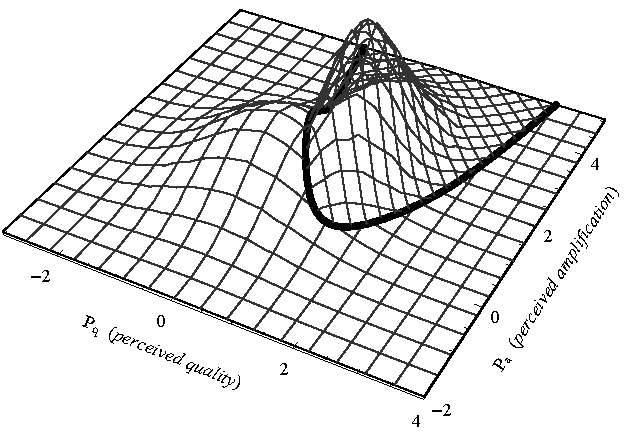
\includegraphics[scale=.55]{"Model 2/Figure 18.pdf}
\caption{Model in equilibrium for Log[$K$]$=0$, $\sigma_{q}=1$ and $\sigma_{a}=1$, showing the perception of a high quality, amplifying sender and a low quality, concealing sender, as well as the optimal threshold-line defining $R_{G}$.}
\label{fig:Model 2/Figure 18.pdf}
\end{center}
\end{figure}

\subsection{Extensive Form}
\label{sec:CueDetectionModelwithObservableAmplification/Extensive Form}

The extensive form of this model is presented in figure~\ref{fig:Model 2/Figure 8.pdf}. Compared to the extensive form in section~\ref{sec:CueDetectionModelwithAmplification/Extensive Form}, the only addition is the receiver's error-prone perception of the level of amplification chosen by the sender.

\begin{figure}[h]
\begin{center}
\leavevmode
\includegraphics[scale=.6]{"Model 2/Figure 8.pdf}
\caption{Extensive form}
\label{fig:Model 2/Figure 8.pdf}
\end{center}
\end{figure}


\subsection{Receiver's Perspective}
\label{sec:CueDetectionModelwithObservableAmplification/Receiver's Perspective}

As discussed in section~\ref{sec:CueDetectionModel/Receiver's Perspective}, the payoff to the receiver is given by integrals of the normal distribution over the appropriate regions $R_{G}$ and $R_{B}$. In this case, it is a double integral over both the perception of quality and the perception of the amplifier.
\begin{equation}
\label{eq:CueDetectionModelwithObservableAmplification/PayoffR}
\begin{array}{rcl}
P_{R}(R_{G}) &=& p \; b_{TP} \displaystyle \iint_{R_{G}} \mathcal{N}(P_{q}, P_{a}, 1, a_{H}, \frac{\sigma_{q}}{a_{H}}, \sigma_{a}) \; dP_{q}dP_{a} +\\
&&p \; b_{FN} \displaystyle \iint_{R_{B}} \mathcal{N}(P_{q}, P_{a}, 1, a_{H}, \frac{\sigma_{q}}{a_{H}}, \sigma_{a}) \; dP_{q}dP_{a} +\\
&&(1-p) \; b_{FP} \displaystyle \iint_{R_{G}} \mathcal{N}(P_{q}, P_{a}, 0, a_{L}, \frac{\sigma_{q}}{a_{L}}, \sigma_{a}) \; dP_{q}dP_{a} +\\
&&(1-p) \; b_{TN} \displaystyle \iint_{R_{B}} \mathcal{N}(P_{q}, P_{a}, 0, a_{L}, \frac{\sigma_{q}}{a_{L}}, \sigma_{a}) \; dP_{q}dP_{a}
\end{array}
\end{equation}

In order to find out what definition of $R_{G}$ gives the receiver the highest payoff, a simple mathematical trick can be applied. We can take a `slice' of the two-dimensional normal distribution by fixing, for example, $P_{q}$. This is shown in figure~\ref{fig:Model 2/Figure 9.pdf}. The mathematics of a bivariate normal distribution is such that, when fixing $P_{q}$ by plugging in a number, the resulting function is a simple, one-dimensional normal distribution. Consequently, we can apply the same method of determining the threshold $t$ as done before in section~\ref{sec:CueDetectionModel/Receiver's Perspective}.

\begin{figure}[!h]
\begin{center}
\leavevmode
\includegraphics[scale=.7]{"Model 2/Figure 9.pdf}
\caption{Slicing the full model}
\label{fig:Model 2/Figure 9.pdf}
\end{center}
\end{figure}

To be more precise, let us take a `sliced' version $\tilde{P}_{R}(\tilde{R}_{G}(P_{q}))$ of the receiver's total payoff $P_{R}(R_{G})$, by simply not performing one of the two integrals.
\begin{equation}
\label{eq:CueDetectionModelwithObservableAmplification/SlicedPayoffR}
P_{R}(R_{G}) = \displaystyle \int \tilde{P}_{R}(\tilde{R}_{G}(P_{q})) \; dP_{q}
\end{equation}

Let us now define $t(P_{q})=\partial \tilde{R}_{G}(P_{q})$ as the boundary of the region `good' for this \mbox{one-dimensional} slice of the payoff. Using differentiation under the integral sign, we obtain equation~\ref{eq:CueDetectionModelwithObservableAmplification/DifferentialPayoffR}.
\begin{equation}
\label{eq:CueDetectionModelwithObservableAmplification/DifferentialPayoffR}
\frac{d}{dt}\tilde{P}_{R}(t)= \frac{(1-p) \; (b_{TP}-b_{FN}) a_{L}}{2 \pi \sigma_{q} \sigma_{a}} e^{-\frac{a_{L}^{2} (0-P_{q})^2}{2 \sigma_{q}^2}-\frac{(a_{L}-t)^2}{2 \sigma_{a}^2}} - \frac{p \; (b_{TN}-b_{FP}) a_{H}}{2 \pi \sigma_{q} \sigma_{a}} e^{-\frac{a_{H}^{2} (1-P_{q})^2}{2 \sigma_{q}^2}-\frac{(a_{H}-t)^2}{2 \sigma_{a}^2}}
\end{equation}

As usual, this can be set equal to zero to find the optimal $t$. This, now, is a function of $P_{q}$, the variable over which we did not perform the integral. Therefore, $t(P_{q})$ describes a threshold-line within the two-dimensional perception-space. This can be seen as the black parabola in figure~\ref{fig:Model 2/Figure 9.pdf}.
\begin{equation}
\label{eq:CueDetectionModelwithObservableAmplification/Threshold}
\begin{array}{rcl}
t(P_{q})&=&\displaystyle \frac{a_{H} + a_{L}}{2} + \frac{a_{H}^{2}\sigma_{a}^{2}}{2 (a_{H} - a_{L}) \sigma_{q}^{2}} - \frac{\sigma_{a}^{2}}{a_{H} - a_{L}} \text{Log} [\bar{K}] -\\
&&\displaystyle \frac{a_{H}^2 \sigma_{a}^2}{(a_{H} - a_{L}) \sigma_{q}^2} P_{q} + \frac{a_{H}+a_{L}}{2} \frac{\sigma_{a}^2}{\sigma_{q}^2} P_{q}^{2}
\end{array}
\end{equation}

The optimal strategy for the receiver consists of a region $R_{G}$ for which it responds to the sender with $G$ and a complementary region $R_{B}$ for which it responds with $B$. These are defined by the threshold $t(P_{q})$, given in equation~\ref{eq:CueDetectionModelwithObservableAmplification/RG}.
\begin{equation}
\label{eq:CueDetectionModelwithObservableAmplification/RG}
R_{G} = \{P_{q}, P_{a} \in \mathbb{R}^{2} : P_{a}>t(P_{q})\}
\end{equation}


\subsection{Sender's Perspective}
\label{sec:CueDetectionModelwithObservableAmplification/Sender's Perspective}

Given the receiver's response-strategy, the sender's payoff is given by equation~\ref{eq:CueDetectionModelwithObservableAmplification/PayoffS}, where the integral is, again, performed over two variables. \mbox{Here, $b_{q} \in \{b_{H}, b_{L}\}$ and $q \in \{1, 0\}$.}
\begin{equation}
\label{eq:CueDetectionModelwithObservableAmplification/PayoffS}
P_{S}(a) = b_{q} \displaystyle \iint_{R_{G}} \mathcal{N}(P_{q}, P_{a}, q, a, \frac{\sigma_{q}}{a}, \sigma_{a}) \; dP_{q}dP_{a}
\end{equation}

We cannot obtain a closed form for this integral. However, we do not necessarily care about the total payoff to the sender, but more about the marginal payoff of amplifying. By examining the derivative of the payoff with respect to $a$, we can find out if a sender should amplify more or less. Without a closed form for the total payoff, it might seem impossible to find an expression for the derivative. Luckily, another mathematical trick can be applied. Let us first `slice' the sender's payoff by not performing one of the integrals.
\begin{equation}
\label{eq:CueDetectionModelwithObservableAmplification/SlicedPayoffS}
P_{S}(a) = \displaystyle \int \tilde{P}_{S}(a) \; dP_{q}
\end{equation}

Due to the fact that derivatives and integrals commute, we can change the derivative of the total payoff to an integral over the derivative of the sliced payoff. This concept is expressed in equation~\ref{eq:CueDetectionModelwithObservableAmplification/DifferentialPayoffS}.
\begin{equation}
\label{eq:CueDetectionModelwithObservableAmplification/DifferentialPayoffS}
\frac{d}{da} P_{S}(a) = \displaystyle \int \frac{d}{da} \tilde{P}_{S}(a) \; dP_{q}
\end{equation}

The derivative of the sliced payoff does have a closed form. Although the integral can still not be solved analytically, we can now use a simple numerical integration over one dimension to estimate the sender's optimal level of amplification.


\subsection{Equilibria}
\label{sec:CueDetectionModelwithObservableAmplification/Equilibria}

The first step in determining the equilibria of this model is to find the various zones of parameter-space. Part of this procedure was explained in section~\ref{sec:CueDetectionModelwithAmplification/Equilibria} and requires us to solve $t(P_{q})=q$ for Log[$K$] where $q \in \{1, 0\}$. In this model, this procedure only makes sense whenever $a_{H}=a_{L}=a$ and the $P_{q}$-dependency of $t(P_{q})$ drops out. This leads to equation~\ref{eq:CueDetectionModelwithObservableAmplification/Zone}.
\begin{equation}
\label{eq:CueDetectionModelwithObservableAmplification/Zone}
Z(\sigma_{q})=\frac{a^{2} (1 - 2 q)}{2 \sigma_{q}^{2}}
\end{equation}

Equation~\ref{eq:CueDetectionModelwithObservableAmplification/Zone} is independent of $\sigma_{a}$ due to the fact that we assumed \mbox{$a_{H}=a_{L}=a$}. Therefore, it can be used to determine only some of the zones of parameter-space. Figure~\ref{fig:Model 2/Figure 10.pdf} depicts these zones within parameter-space and their associated equilibria, which depend on $\sigma_{q}$ and Log[$K$]. Numerical estimations were used to determine the $\sigma_{a}$-dependency and the associated zones are also depicted in figure~\ref{fig:Model 2/Figure 10.pdf} for $\sigma_{a}=6$. When $\sigma_{a} \to \infty$, this model reduces to the one of section~\ref{sec:CueDetectionModelwithAmplification/Equilibria} and figure~\ref{fig:Model 2/Figure 10.pdf} becomes equal to figure~\ref{fig:Model 2/Figure 4.pdf}. As such, the interpretation of the various zones follows very similar lines to the discussion in section~\ref{sec:CueDetectionModelwithAmplification/Equilibria}.

\begin{figure}[!h]
\begin{center}
\leavevmode
\includegraphics[scale=.8]{"Model 2/Figure 10.pdf}
\caption{Equilibria for $\sigma_{a}=6$, $a_{\text{Min}}=1$ and $a_{\text{Max}}=2$}
\label{fig:Model 2/Figure 10.pdf}
\end{center}
\end{figure}

The model predicts that, for Log[$K$]$=1$ and $\sigma_{q}=3$, both high and low quality senders will amplify their quality cue to the maximum possible level. For a high level of $K$, the receiver is very lenient, responding favourably to a wide range of perceived qualities and perceived levels of amplification. Therefore, both types of senders benefit from amplifying. With identical levels of amplification, the behaviour of the receiver is the same as that predicted by our previous model, in section~\ref{sec:Cue Detection Model with Amplification}, in which the level of amplification was unobservable.

If $K$ becomes lower, but $\sigma_{q}$ remains high, falling within the light-striped zone or the circle zone of figure~\ref{fig:Model 2/Figure 10.pdf}, the receiver is less lenient. In this case, the low quality sender will wish to amplify, but only up to a certain level. As the low quality sender increases its level of amplification, the receiver can observe its low quality cue more accurately. However, as the level of amplification is observable to the receiver in this model, and high quality senders amplify maximally, the receiver has developed a preference for higher levels of amplification. In this zone of parameter-space, it pays low quality senders to amplify their cue partially. Compared to the model of section~\ref{sec:Cue Detection Model with Amplification}, the range of parameters for which the low quality sender amplifies partially is much larger and is not restricted to high values of $K$.

If Log[$K$] is negative and $\sigma_{q}$ is low, the receiver is relatively cautious in its response to the sender. This may even lead to the high quality sender not wanting to amplify its cue. For the dark-striped zone and the circle zone, two equilibria are possible and the one the model ends up in depends on the starting point of the dynamics and on the basins of attraction of the equilibria.

As just explained, there is a zone for which a low quality sender will want to amplify its cue, at least partially. Using equation~\ref{eq:CueDetectionModelwithObservableAmplification/DifferentialPayoffS}, numerical estimations give us the optimal value of this level of amplification. This can be seen in figure~\ref{fig:Model 2/Figure 12.pdf}. Furthermore, there is a zone in parameter-space for which two equilibria are possible. This means there must be an unstable equilibrium separating the two. Using, again, equation~\ref{eq:CueDetectionModelwithObservableAmplification/DifferentialPayoffS}, numerical estimation can determine the value of this unstable equilbrium. If the level of amplification of the high quality sender starts off below this value, it will decrease further to the minimum value $a_{\text{Min}}$. If, however, it started off above this unstable equilibrium, it will increase further to the maximum possible value $a_{\text{Max}}$. Figure~\ref{fig:Model 2/Figure 1112} plots these two numerical estimations.

\begin{figure}[!h]
\captionsetup{width=380pt}
\begin{center}
\subfloat[Unstable equilibrium $a_{U}$ for Log($K$)$=-2$]{\label{fig:Model 2/Figure 11.pdf}\includegraphics[scale=.5]{"Model 2/Figure 11.pdf}}
\hspace{6mm}
\subfloat[Stable equilibrium $a_{L}$ for Log($K$)$=0$]{\label{fig:Model 2/Figure 12.pdf}\includegraphics[scale=.5]{"Model 2/Figure 12.pdf}}
\caption{The unstable equilibrium value of amplification $a_{U}$ for the high quality sender and the stable equilibrium value of amplification, $a_{L}$, for the low quality sender, taking $a_{\text{Min}}=1$ and $a_{\text{Max}}=2$.}
\label{fig:Model 2/Figure 1112}
\end{center}
\end{figure}

Similar to our game-theoretical model of observable amplification of section~\ref{sec:Cue Game with Observable Amplification}, it is interesting to see how the levels of amplification change as $\sigma_{a}$ decreases. The variable $\sigma_{a}$ is a measure of the receiver's ability to detect the level of amplification used by the sender. Starting from the unobservable amplification model of section~\ref{sec:Cue Detection Model with Amplification}, receivers may evolve the ability to assess the sender's quality via their use of an amplifying display. Figure~\ref{fig:Model 2/Figure 1314151617} plots the relative levels of amplification for various parameter values. The discussion of the information content of the two cues in figure~\ref{fig:Model 2/Figure 1314151617} follows similar lines to the discussion in section~\ref{sec:Cue Game with Observable Amplification/Equilibria}.

The variable $\Delta a$ is defined as in equation~\ref{eq:Deltaa}. It represents the relative difference between the level of amplification of the high and the low quality sender.
\begin{equation}
\label{eq:Deltaa}
\Delta a = \frac{a_{\text{Max}}-a}{a_{\text{Max}}-a_{\text{Min}}}
\end{equation}

Figure~\ref{fig:Model 2/Figure 1314151617} shows that, as $\sigma_{a}$ decreases, low quality senders will amplify at a higher level. Furthermore, as Log[$K$] increases, the receiver has a higher incentive to respond favourably and the low quality sender is also more likely to amplify its cue. This is a similar result to the one found in section~\ref{sec:Cue Game with Observable Amplification/Equilibria}. Figure~\ref{fig:Model 2/Figure 1314151617} also shows that, as $\sigma_{q}$ increases, the receiver pays relatively more attention to the use of the amplifier by the sender, resulting in low quality senders choosing a higher level of amplification. A visual representation of the model in its ($a_{\text{Max}}$,~$a_{\text{Min}}$)-equilibrium is given in figure~\ref{fig:Model 2/Figure 18.pdf}. It shows the perception of quality and amplification following two-dimensional normal distributions, as well as the optimal threshold-function separating $R_{G}$ and $R_{B}$.
\begin{figure}[!h]
\subfloat[Log($K$)$=1$, $\sigma_{q}=1$]{\label{fig:Model 2/Figure 13.pdf}\includegraphics[scale=.49]{"Model 2/Figure 13.pdf}}
\hfill
\subfloat[Log($K$)$=0$, $\sigma_{q}=1$]{\label{fig:Model 2/Figure 14.pdf}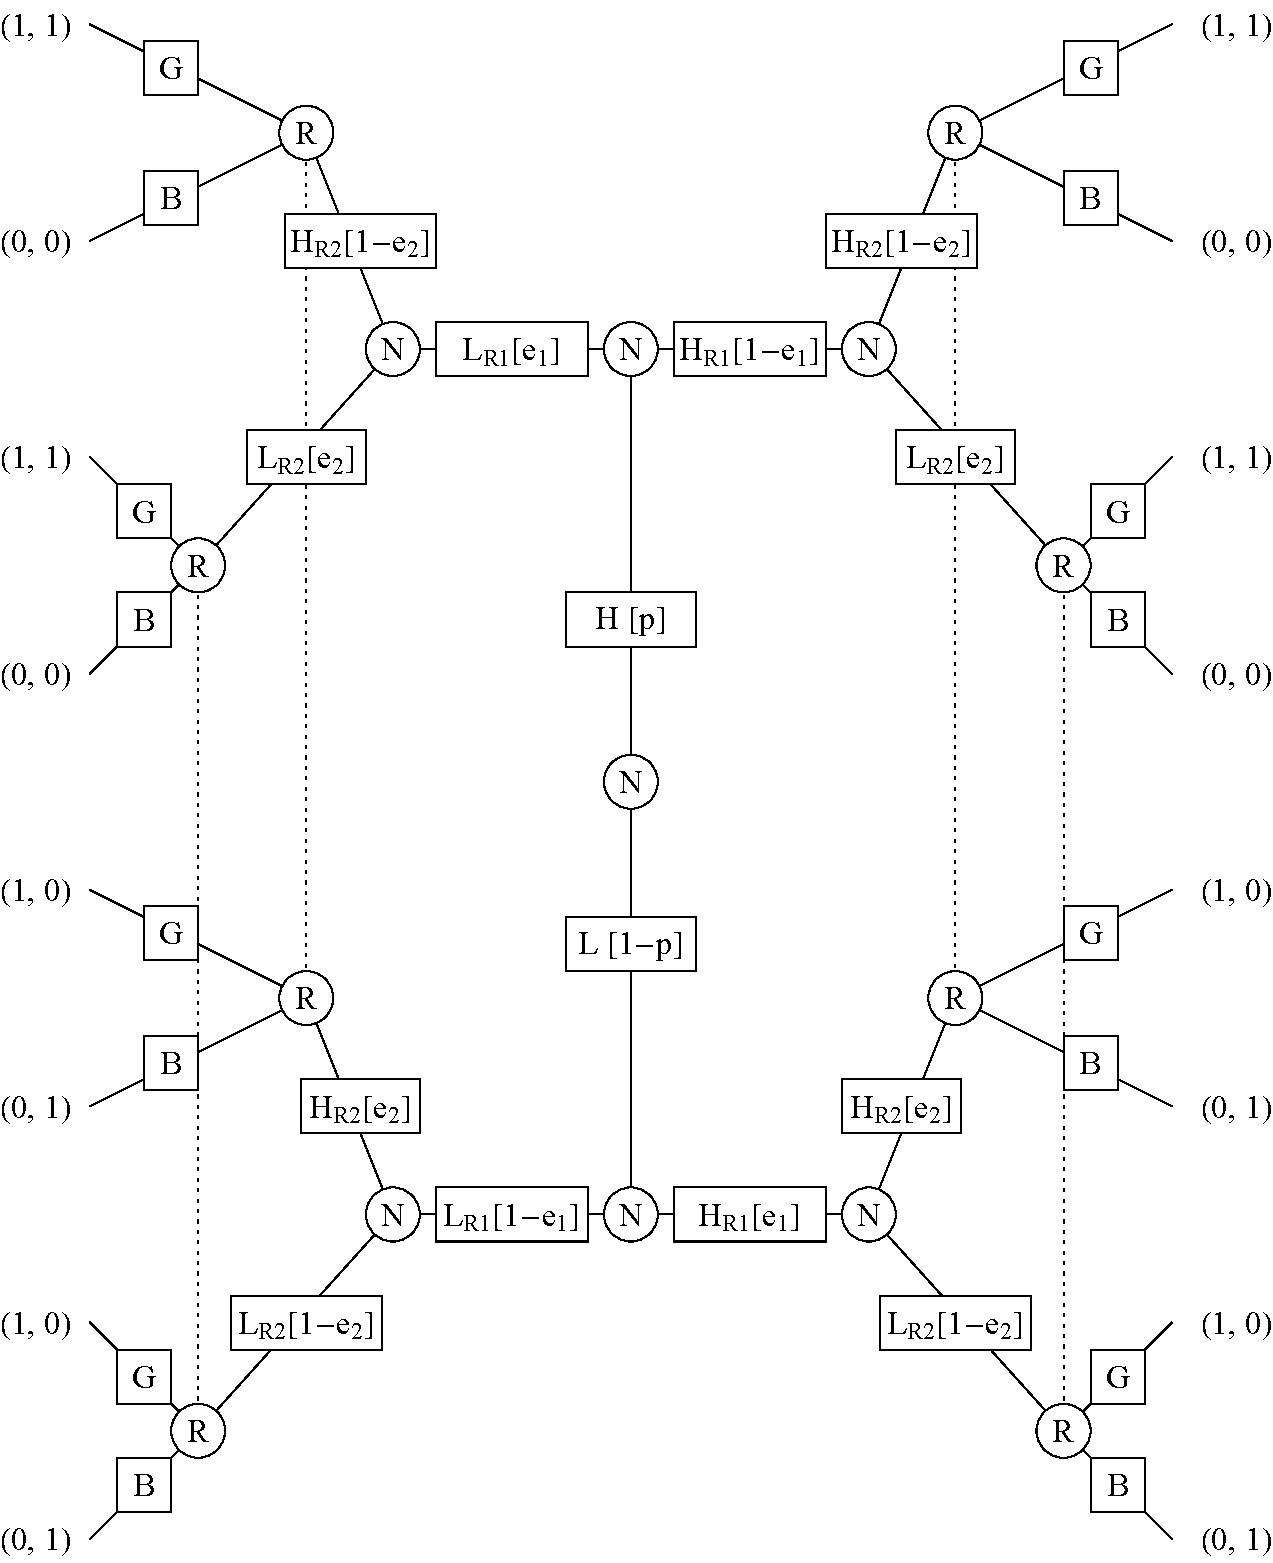
\includegraphics[scale=.49]{"Model 2/Figure 14.pdf}}\\[-3mm]
\subfloat[Log($K$)$=-1$, $\sigma_{q}=1$]{\label{fig:Model 2/Figure 15.pdf}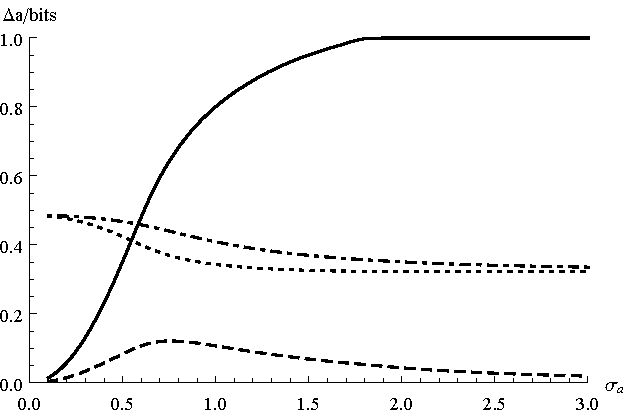
\includegraphics[scale=.49]{"Model 2/Figure 15.pdf}}
\hfill
\subfloat[Log($K$)$=0$, $\sigma_{q}=0.6$]{\label{fig:Model 2/Figure 16.pdf}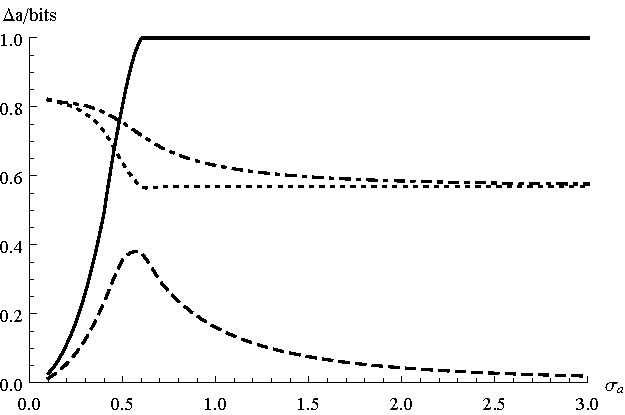
\includegraphics[scale=.49]{"Model 2/Figure 16.pdf}}\\[-3mm]
\subfloat[Log($K$)$=0$, $\sigma_{q}=1.7$]{\label{fig:Model 2/Figure 17.pdf}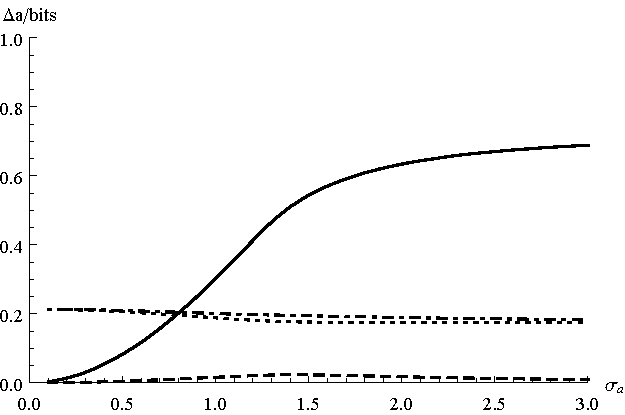
\includegraphics[scale=.5]{"Model 2/Figure 17.pdf}}
\hfill
\begin{minipage}[t]{.45\textwidth}
\captionsetup{width=250pt}
\vspace{-45mm}
\caption{As $\sigma_{a}$ decreases, the receiver becomes better at assessing the level of amplification chosen by the sender. These figures show the equilibrium of the relative difference in these levels for the high and the low quality sender, $\Delta a$, as a function of $\sigma_{a}$, as well as the information content in bits of the two cues obtained by the receiver: quality information (dotted), amplifier information (dashed) and both cues combined (dot-dashed).}
\label{fig:Model 2/Figure 1314151617}
\end{minipage}
\end{figure}


\subsection{Example}
\label{sec:CueDetectionModelwithObservableAmplification/Example}

\enlargethispage{6mm}

In pipefish, \textit{Syngnathus typhle}, sex roles are reversed and it is the males who select females. Female body size is an important measure for males, as larger females can produce larger, energy-rich eggs. Females have a sexual display, a cross-wise striped pattern along their body~\cite{Berglund2000}. They can increase or decrease the contrast of this pattern within a minute, allowing full dependency on their own quality. In an experiment with students, it has been shown that this pattern can facilitate the assessment of width of a rectangle. If the same applies to pipefish, males will find it easier to assess body size of females who show this amplifying display. In an experiment manipulating the display by painting females and by controlling for sexual dance-movements by sedating them and moving them in a dance-like fashion by a motor, males preferred the painted females over the control group~\cite{Berglund2001}. This suggests that, if the pattern indeed functions as an amplifier, it is an easily observable trait for which there is direct male preference.


\newpage\clearpage


\section{Signal Detection Model}
\label{sec:Signal Detection Model}
\subsection{Assumptions}
\label{sec:SignalDetectionModel/Assumptions}

In this section, we will use the mathematical framework developed in the previous sections to examine handicap signalling. We will assume the sender has the ability to signal to the receiver, at a cost which is dependent on its quality. In particular, let the cost function of signalling for a high quality sender always be below the cost function of the low quality sender, $c_{H}(s)<c_{L}(s) \; \forall \; s$. The receiver does not have the ability to detect the quality of the sender directly, but observes the signal from the sender with some error. This error is assumed to follow a normal distribution with variance $\sigma^{2}_{s}$.

\begin{equation}
\label{eq:SignalDetectionModel/Normal}
\mathcal{N}(P_{s}, s, \sigma_{s}) = \frac{1}{\sqrt{2 \pi} \sigma_{s}} e^{-\frac{(P_{s}-s)^2}{2 \sigma_{s}^2}}
\end{equation}

Either the relative difference between $c_{H}$ and $c_{L}$ or $\sigma_{s}$ sets the scale in this model, which means we can fix one of these parameters. Let us set $\sigma_{s}=1$ and allow the cost functions to be the free parameters which determine the sender's incentive to signal to the receiver.

Figure~\ref{fig:Model 2/Figure 27.pdf} shows the perception-axis with two normal distributions representing a high and a low quality sender.

\begin{figure}[!h]
\captionsetup{width=300pt}
\begin{center}
\leavevmode
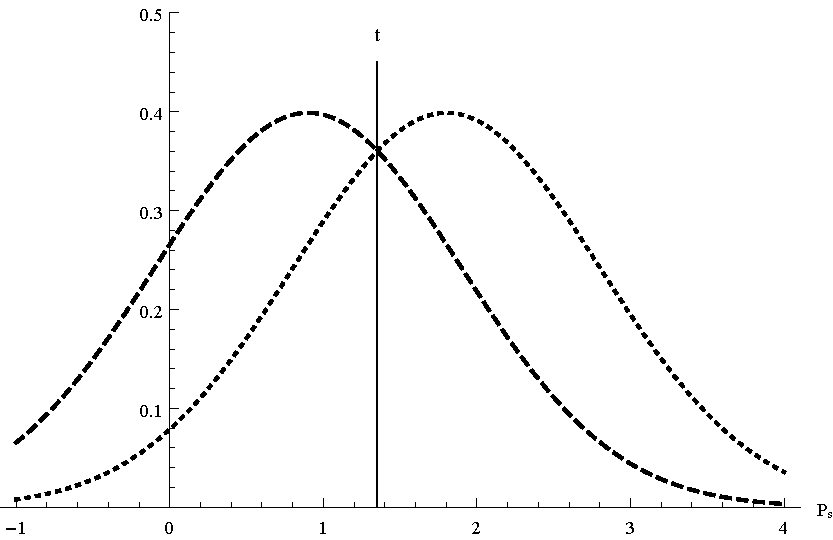
\includegraphics[scale=.65]{"Model 2/Figure 27.pdf}
\caption{Model in equilibrium for Log[$K$]$=0$, $\sigma_{s}=1$, $c_{H}=0.10$ and $c_{L}=0.20$, showing the perception of a high quality sender (dotted) and a low quality sender (dashed), as well as the optimal threshold at $t=1.35$.}
\label{fig:Model 2/Figure 27.pdf}
\end{center}
\end{figure}

\subsection{Extensive Form}
\label{sec:SignalDetectionModel/Extensive Form}

Figure~\ref{fig:Model 2/Figure 19.pdf} shows the extensive form of this model. After Nature has made the random choice between a high and a low quality sender, the sender decides on a level of signalling~$s$. This level is not directly observable to the receiver, as indicated by the dotted lines. The cost functions are now included in the payoff of the sender.

\begin{figure}[h]
\begin{center}
\leavevmode
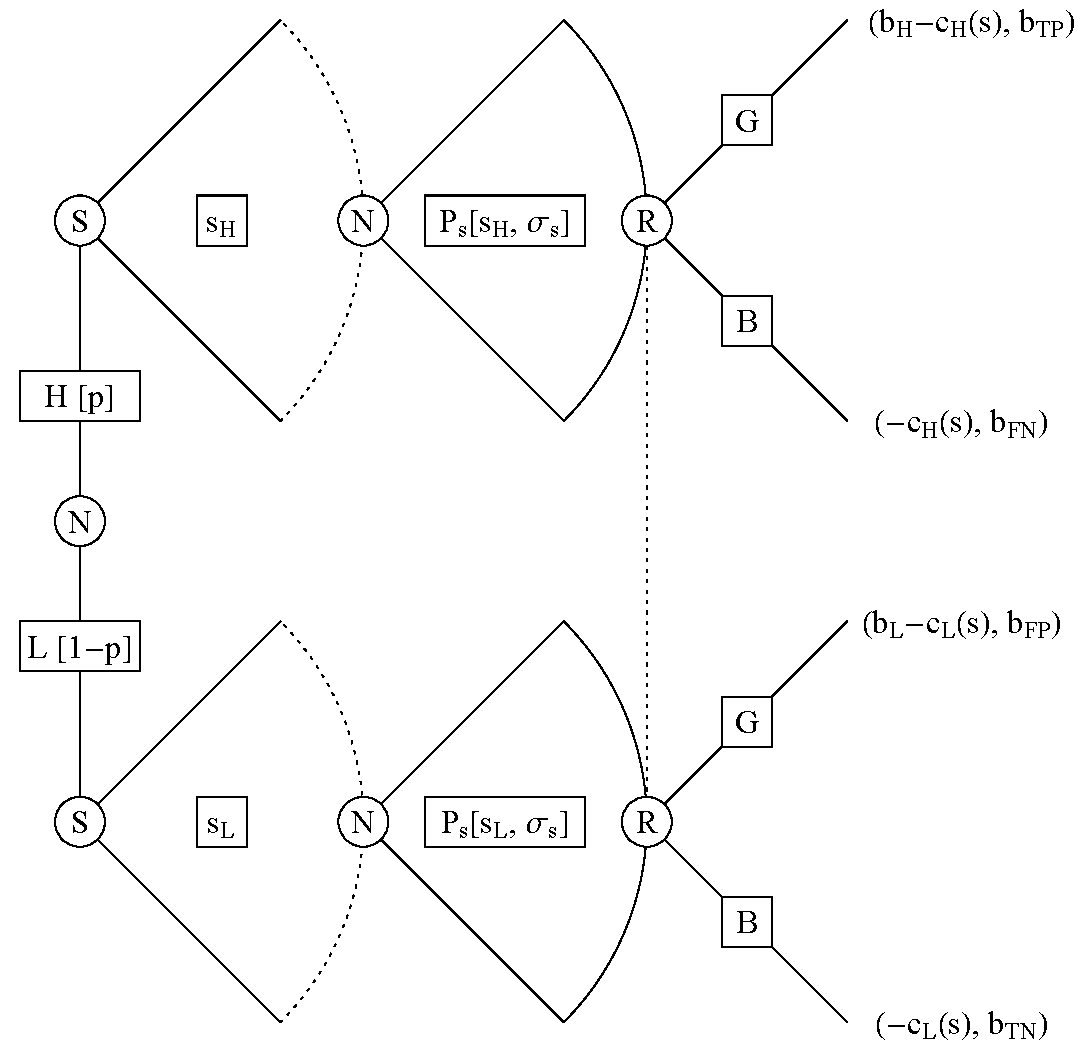
\includegraphics[scale=.65]{"Model 2/Figure 19.pdf}
\caption{Extensive form}
\label{fig:Model 2/Figure 19.pdf}
\end{center}
\end{figure}


\subsection{Receiver's Perspective}
\label{sec:SignalDetectionModel/Receiver's Perspective}

The detection of a signal is very similar to the detection of a quality cue for the receiver. The following mathematics is almost identical to that of section~\ref{sec:CueDetectionModel/Receiver's Perspective}. Equation~\ref{eq:SignalDetectionModel/PayoffR} gives the receiver's payoff.
\begin{equation}
\label{eq:SignalDetectionModel/PayoffR}
\begin{array}{rcl}
P_{R}(R_{G}) &=& p \; b_{TP} \displaystyle \int_{R_{G}} \mathcal{N}(P_{s}, s_{H}, \sigma_{s}) \; dP_{s} +\\
&&p \; b_{FN} \displaystyle \int_{R_{B}} \mathcal{N}(P_{s}, s_{H}, \sigma_{s}) \; dP_{s} +\\
&&(1-p) \; b_{FP} \displaystyle \int_{R_{G}} \mathcal{N}(P_{s}, s_{L}, \sigma_{s}) \; dP_{s} +\\
&&(1-p) \; b_{TN} \displaystyle \int_{R_{B}} \mathcal{N}(P_{s}, s_{L}, \sigma_{s}) \; dP_{s}
\end{array}
\end{equation}

Taking again $t=\partial R_{G}$ as the boundary of the region `good', we use differentiation under the integral sign to obtain equation~\ref{eq:SignalDetectionModel/DifferentialPayoffR}.
\begin{equation}
\label{eq:SignalDetectionModel/DifferentialPayoffR}
\frac{d}{dt}P_{R}(t)= \frac{(1-p) \; (b_{TP}-b_{FN})}{\sqrt{2 \pi} \sigma_{s}} e^{-\frac{(s_{H}-t)^2}{2 \sigma_{s}^2}} - \frac{p \; (b_{TN}-b_{FP})}{\sqrt{2 \pi} \sigma_{s}} e^{-\frac{(s_{L}-t)^2}{2 \sigma_{s}^2}}
\end{equation}

The optimal threshold $t$ depends on the level of signalling by the high and the low quality sender.
\begin{equation}
\label{eq:SignalDetectionModel/Threshold}
t=\frac{s_{H}+s_{L}}{2}-\frac{\sigma_{s}^2 \text{Log}[K]}{s_{H}-s_{L}}
\end{equation}

This threshold defines how the receiver should best responds to any observed level of signalling.
\begin{equation}
\label{eq:SignalDetectionModel/RG}
R_{G} = \{P_{s} \in \mathbb{R} : P_{s}>t\}
\end{equation}


\subsection{Sender's Perspective}
\label{sec:SignalDetectionModel/Sender's Perspective}

The payoff to the sender is given by the integral over $R_{G}$, subtracting the cost of signalling. Here, $b_{q} \in \{b_{H}, b_{L}\}$ and $c_{q} \in \{c_{H}, c_{L}\}$.
\begin{equation}
\label{eq:SignalDetectionModel/PayoffS}
P_{S}(s) = b_{q} \displaystyle \int_{R_{G}} \mathcal{N}(P_{s}, s, \sigma_{s}) \; dP_{s}-c_{q}(s)
\end{equation}

A general cost function can be defined via its Taylor-expansion, as in equation~\ref{eq:SignalDetectionModel/CostFunction}.
\begin{equation}
\label{eq:SignalDetectionModel/CostFunction}
c(s)=\sum_{i=0}^{\infty} c_{i} \; s^{i}
\end{equation}

It makes sense for the cost function to start at zero and be increasing at an increasing rate. As such, let us take $c_{0}=c_{1}=0$ and $c_{i} \geq 0 \; \forall \; i$. The simplest of these functions is given in equation~\ref{eq:SignalDetectionModel/CostFunction2}.
\begin{equation}
\label{eq:SignalDetectionModel/CostFunction2}
c_{q}(s)=c_{q} \, s^{2}
\end{equation}

By differentiating the sender's payoff, we obtain an expression for the marginal payoff of signalling. Equation~\ref{eq:SignalDetectionModel/DifferentialPayoffS} is used determine numerically the optimal level of signalling for the high and the low quality sender.
\begin{equation}
\label{eq:SignalDetectionModel/DifferentialPayoffS}
\frac{d}{ds} P_{S}(s) = \frac{b_{q}}{\sqrt{2 \pi} \sigma_{s}} e^{-\frac{(s-t)^2}{2 \sigma_{s}^2}} - 2 \, c_{q} \, s
\end{equation}


\subsection{Equilibria}
\label{sec:SignalDetectionModel/Equilibria}

An equilibrium of this model is reached when neither the high nor the low quality sender has an incentive to change its level of signalling, given the receiver's optimal strategy $R_{G}$. Before we turn to these calculations, let us examine equation~\ref{eq:SignalDetectionModel/DifferentialPayoffS} more carefully.

At equilibrium, the marginal cost and the marginal benefit of signalling should equate. Therefore, the optimal level of signalling is not determined by the cost $c_{H}$ or $c_{L}$, but by the relative costs $\frac{c_{H}}{b_{H}}$ and $\frac{c_{L}}{b_{L}}$. Let us now define the ratio between these two relative costs, in equation~\ref{eq:SignalDetectionModel/RatioCost}.
\begin{equation}
\label{eq:SignalDetectionModel/RatioCost}
r_{c} = \frac{c_{H}}{c_{L}} \frac{b_{L}}{b_{H}}
\end{equation}

Furthermore, at equilibrium, the marginal payoff of signalling for the high quality sender should be equal to the marginal payoff for the low quality sender, both of which are zero. The relative marginal benefit of signalling depends on the position of the threshold $t$. This can be seen in figure~\ref{fig:Model 2/Figure 27.pdf}. Given the receiver's optimal strategy, the ratio between the marginal benefit of the high quality sender and the low quality sender is equal to $K$. This provides us with a simple, analytical expression for the ratio between the levels of signalling for the high and the low quality sender, i.e. $s_{L}=r s_{H}$ where $0 \leq r \leq 1$.
\begin{equation}
\label{eq:SignalDetectionModel/Ratio}
r=r_{c} \, K
\end{equation}

Now that we know this ratio, we can reduce the two unknown variables $s_{H}$ and $s_{L}$ to a single unknown variable $s_{r}$. This allows us to visualise the costs and the benefits associated with signalling in a simple plot. Figure~\ref{fig:Model 2/Figure 202122} shows these payoffs for various parameters.
\begin{figure}[!h]
\begin{center}
\subfloat[Log($K$)$=0$]{\label{fig:Model 2/Figure 20.pdf}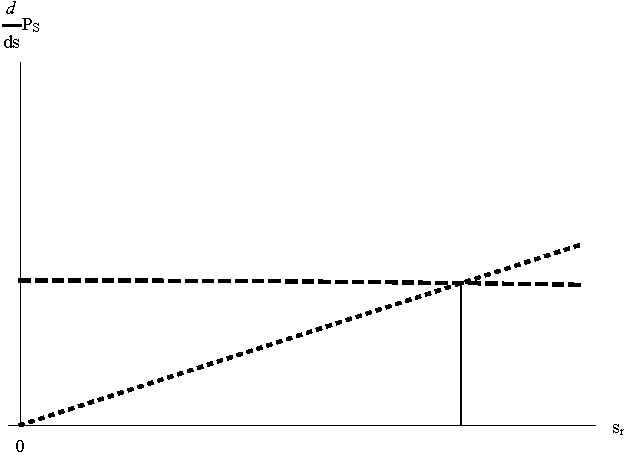
\includegraphics[scale=.48]{"Model 2/Figure 20.pdf}}
\hspace{1mm}
\subfloat[Log($K$)$=0.12$]{\label{fig:Model 2/Figure 21.pdf}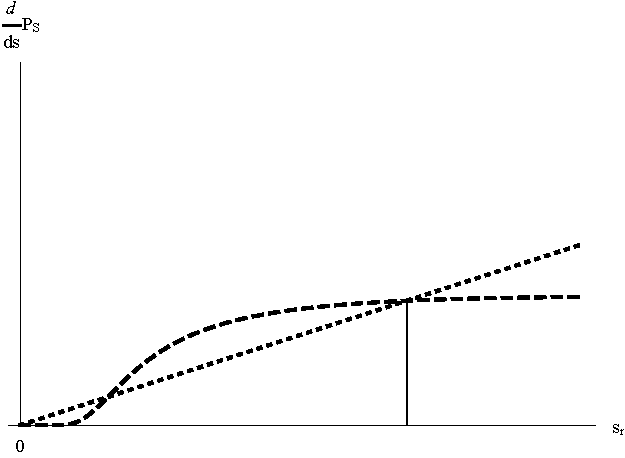
\includegraphics[scale=.48]{"Model 2/Figure 21.pdf}}
\hspace{1mm}
\subfloat[Log($K$)$=0.28$]{\label{fig:Model 2/Figure 22.pdf}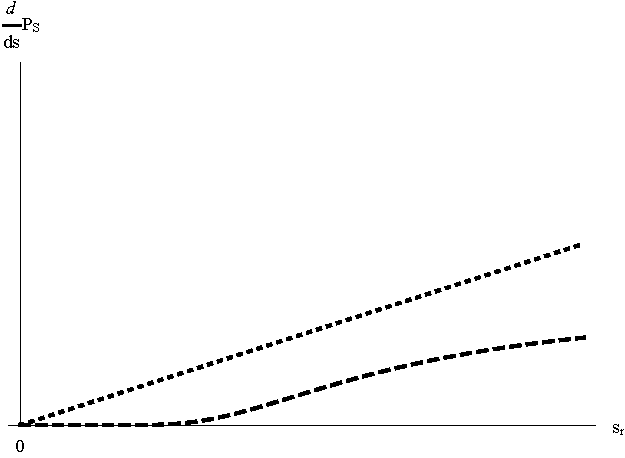
\includegraphics[scale=.48]{"Model 2/Figure 22.pdf}}
\caption{Cost (dotted) and benefit (dashed) functions}
\label{fig:Model 2/Figure 202122}
\end{center}
\end{figure}

What can be deduced from figure~\ref{fig:Model 2/Figure 202122} is that, for some part of parameter-space, no signalling will occur. In particular, if Log[$K$] deviates too much from zero, the cost of signalling is higher than its benefit and neither high nor low quality sender will want to signal. If, however, Log[$K$] is close to zero, the signalling equilibrium is stable. In this case, the non-signalling equilibrium is also stable, giving two possible end-points for our model.

Figure~\ref{fig:Model 2/Figure 23.pdf} shows parameter-space for our two combined parameters Log[$K$] and $r_{c}$. The fact that signalling is not a stable equilibrium whenever Log[$K$] deviates slightly from zero is strange. It is a result of the way the benefit function changes as Log[$K$] changes. In particular, the marginal benefit of signalling is equal to the height of the normal distribution at the threshold $t$. For values of Log[$K$] which are not close to zero, this threshold blows up to either $\infty$ or $-\infty$ whenever the level of signalling is low. This can be seen clearly in equation~\ref{eq:SignalDetectionModel/Threshold}. Consequently, with a very high or a very low threshold, the benefit of signalling becomes virtually zero. The results is that signalling is not stable for a wide range of parameters in this model. This should be taken as an artefact of the model, however, caused by the unrealistic assumption that the level of signalling is the only source of information on which the receiver can base its assessment of quality. In section~\ref{sec:Cue and Signal Detection Model}, we will see a more realistic model which overcomes this problem.

\begin{figure}[h]
\begin{center}
\leavevmode
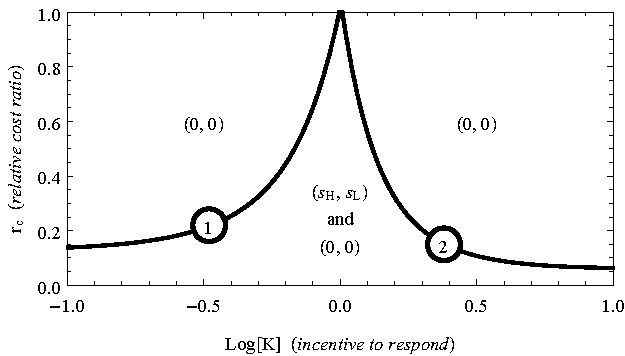
\includegraphics[scale=.9]{"Model 2/Figure 23.pdf}
\caption{Equilibria}
\label{fig:Model 2/Figure 23.pdf}
\end{center}
\end{figure}

Figure~\ref{fig:Model 2/Figure 23.pdf} is obtained via numerical estimations and the precise zones for which signalling does or does not occur are not completely given by parameters Log[$K$] and $r_{c}$. The zones change slightly for different values of $\frac{c_{H}}{b_{H}}$ and $\frac{c_{L}}{b_{L}}$, but the general shape of the zones remains the same. The reason for using $r_{c}$ as a parameter is to conform to the results of section~\ref{sec:Cue and Signal Detection Model}.

Assuming that the signalling equilibrium is stable, we can determine the level at which each type of sender will signal as a function of the costs. Figure~\ref{fig:Model 2/Figure 2425} shows these levels for the high and the low quality sender, having set $b_{H}=b_{L}=1$.
\begin{figure}[h]
\captionsetup{width=380pt}
\begin{center}
\subfloat[Level of signalling for the high quality sender]{\label{fig:Model 2/Figure 24.pdf}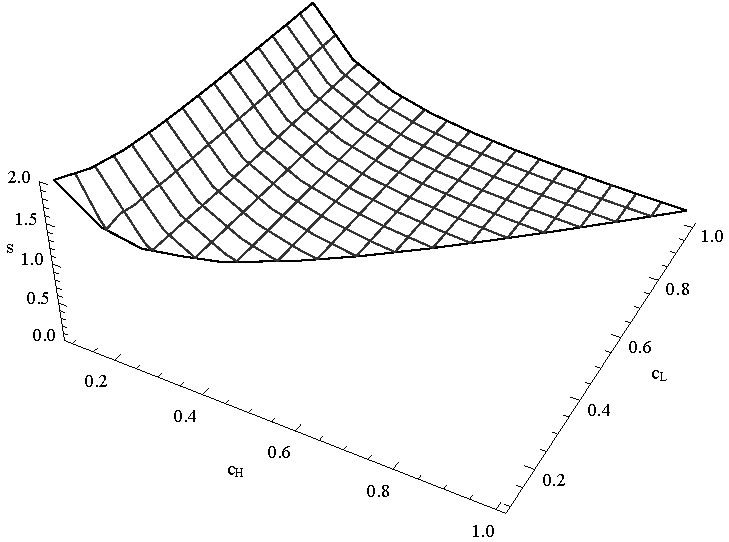
\includegraphics[scale=.58]{"Model 2/Figure 24.pdf}}
\hspace{10mm}
\subfloat[Level of signalling for the low quality sender]{\label{fig:Model 2/Figure 25.pdf}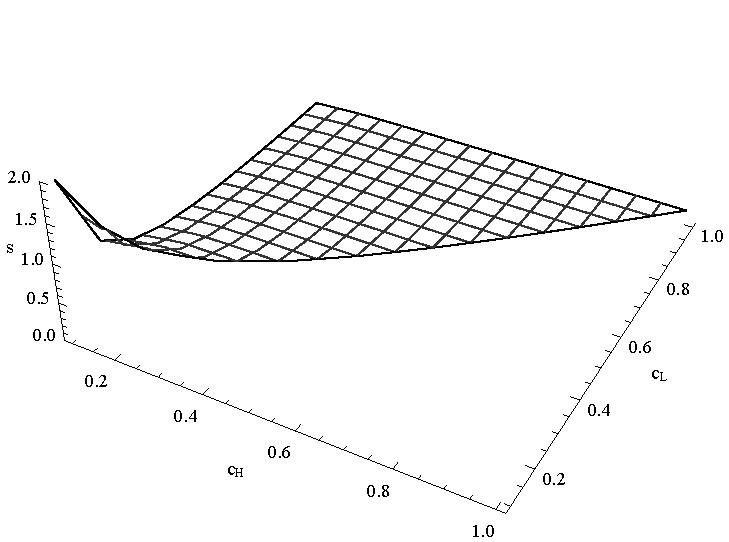
\includegraphics[scale=.58]{"Model 2/Figure 25.pdf}}
\caption{Levels of signalling as a function of the cost with Log[$K$]$=0$ and $\sigma_{s}=1$, keeping $c_{H}<c_{L}$.}
\label{fig:Model 2/Figure 2425}
\end{center}
\end{figure}

\newpage

It may also be interesting to plot this same information in a two-dimensional figure. In this case, we can include the information content of the signal as well. This is done in figure~\ref{fig:Model 2/Figure 26.pdf}.
\begin{figure}[!h]
\captionsetup{width=250pt}
\begin{center}
\leavevmode
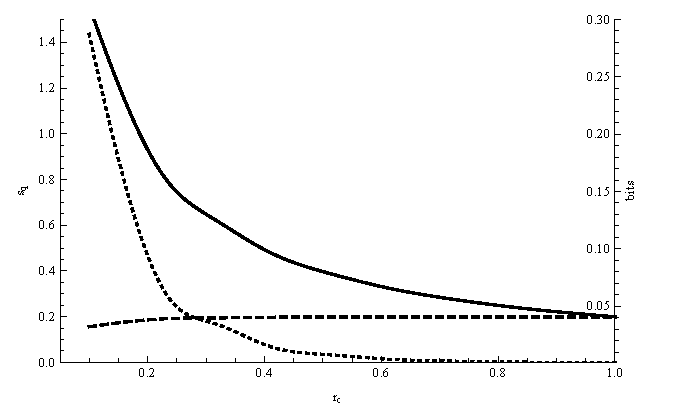
\includegraphics[scale=1]{"Model 2/Figure 26.pdf}
\caption{Level of signalling for the high quality sender (thick) and low quality sender (dashed) as a function of the relative cost, as well as the information content (dotted), when $c_{L}=1$.}
\label{fig:Model 2/Figure 26.pdf}
\end{center}
\end{figure}


\subsection{Example}
\label{sec:SignalDetectionModel/Example}

In field crickets, \textit{Gryilus lineaticeps}, male chirp rate, duration, and amplitude all influence female mate choice; females prefer higher chirp rates, longer chirp durations, and higher chirp amplitudes~\cite{Wagner1996}. The production of calling songs is shown to be energetically costly. During the singing, male crickets significantly increased oxygen consumption~\cite{Hoback1997}. The ability to chirp is also dependent on the condition of the male. In an experiment, males on a high-nutrition feeding regime both called more frequently and called at higher chirp rates then the control group~\cite{Wagner1999}. As the weight of the well-fed males did not increase compared to the control group, this suggested that males invest any excess energy above their basic maintenance requirements in the production of call types that increase their attractiveness to females. Therefore, chirping entails a differential, condition-dependent cost and it may be suggested that the display honestly signals foraging ability as well as current condition. Another cost of chirping has been found. Male crickets are often attacked by parasitoid tachinid flies, \textit{Ormia ochracea}, that locate males through their calls. Female flies deposit larvae on crickets which burrow into and feed on them, killing the cricket. Chirp rate, duration, and amplitude all influenced the probability of fly attraction, creating an additional cost to the singing~\cite{Wagner1996}. Well-fed, high quality male crickets take on these risks, chirp more and attract more females.

\newpage\clearpage


\section{Cue and Signal Detection Model}
\label{sec:Cue and Signal Detection Model}
\subsection{Assumptions}
\label{sec:CueandSignalDetectionModel/Assumptions}

The model of section~\ref{sec:Signal Detection Model} showed that, over a fairly restricted range of parameters, signalling can be a stable equilibrium. The model was unrealistic, however, in its assumption that the level of signalling was the only basis on which the receiver could assess the sender's quality. In nature, animals must surely be able to combine multiple inputs to arrive at an overall assessment of the observed quality~\cite{Jennions1997, Candolin2003}. As such, let us now extend the previous model by including a quality cue, next to the signal. We assume the sender has the ability to signal to the receiver, at a cost which is dependent on its quality. The receiver has some ability to detect the quality of the sender, as well as the signal from the sender. This follows a bivariate normal distribution.
\begin{equation}
\label{eq:CueandSignalDetectionModel/Normal}
\mathcal{N}(P_{q}, P_{s}, q, s, \sigma_{q}, \sigma_{s}) = \frac{1}{2 \pi \sigma_{q} \sigma_{s}} e^{-\frac{(P_{q}-q)^2}{2 \sigma_{q}^2}-\frac{(P_{s}-s)^2}{2 \sigma_{s}^2}}
\end{equation}

As before, the scale in the perception of quality in this model is set by either the distance between $q_{H}$ and $q_{L}$ or $\sigma_{q}$. The scale in the perception of the signal is set by the relative difference between $c_{H}$ and $c_{L}$ or by $\sigma_{s}$. This means we can fix several of these parameters. Let us set $q_{H}=1$ and $q_{L}=0$ and allow $\sigma_{q}$ to be the free parameter which defines the receiver's ability to detect the quality of the sender. Let us also set $\sigma_{s}=1$ and allow the cost functions to be the free parameters which determine the sender's incentive to signal to the receiver.

Figure~\ref{fig:Model 2/Figure 36.pdf} shows the two-dimensional perception-axes with two normal distributions representing a high and a low quality sender.

\begin{figure}[h]
\captionsetup{width=350pt}
\begin{center}
\leavevmode
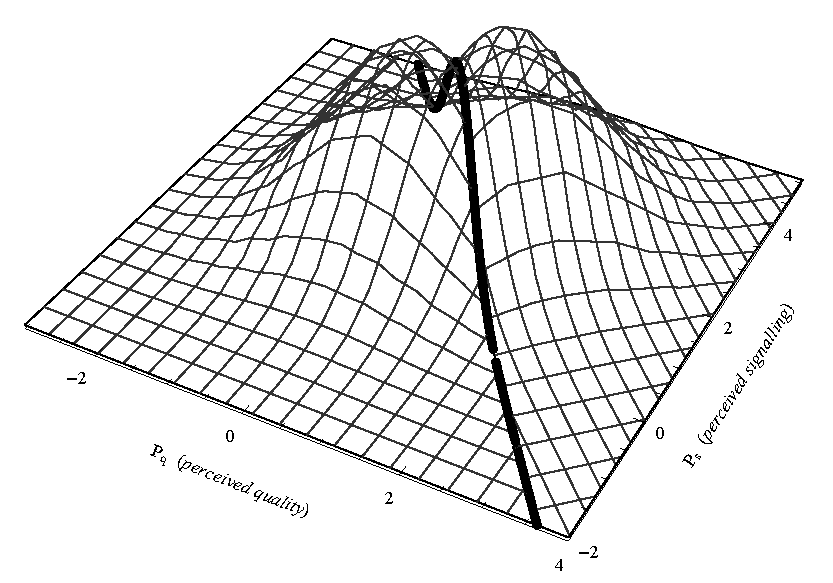
\includegraphics[scale=.7]{"Model 2/Figure 36.pdf}
\caption{Model in equilibrium for Log[$K$]$=0$, $\sigma_{s}=1$, $c_{H}=0.01$ and $c_{L}=0.02$, showing the perception of a high quality sender and a low quality sender, as well as the optimal threshold-line.}
\label{fig:Model 2/Figure 36.pdf}
\end{center}
\end{figure}


\subsection{Extensive Form}
\label{sec:CueandSignalDetectionModel/Extensive Form}

The extensive form of this model is presented in figure~\ref{fig:Model 2/Figure 28.pdf}. In comparison to the previous model, the only addition is the receiver's error-prone perception of the sender's quality~cue.
\begin{figure}[!h]
\begin{center}
\leavevmode
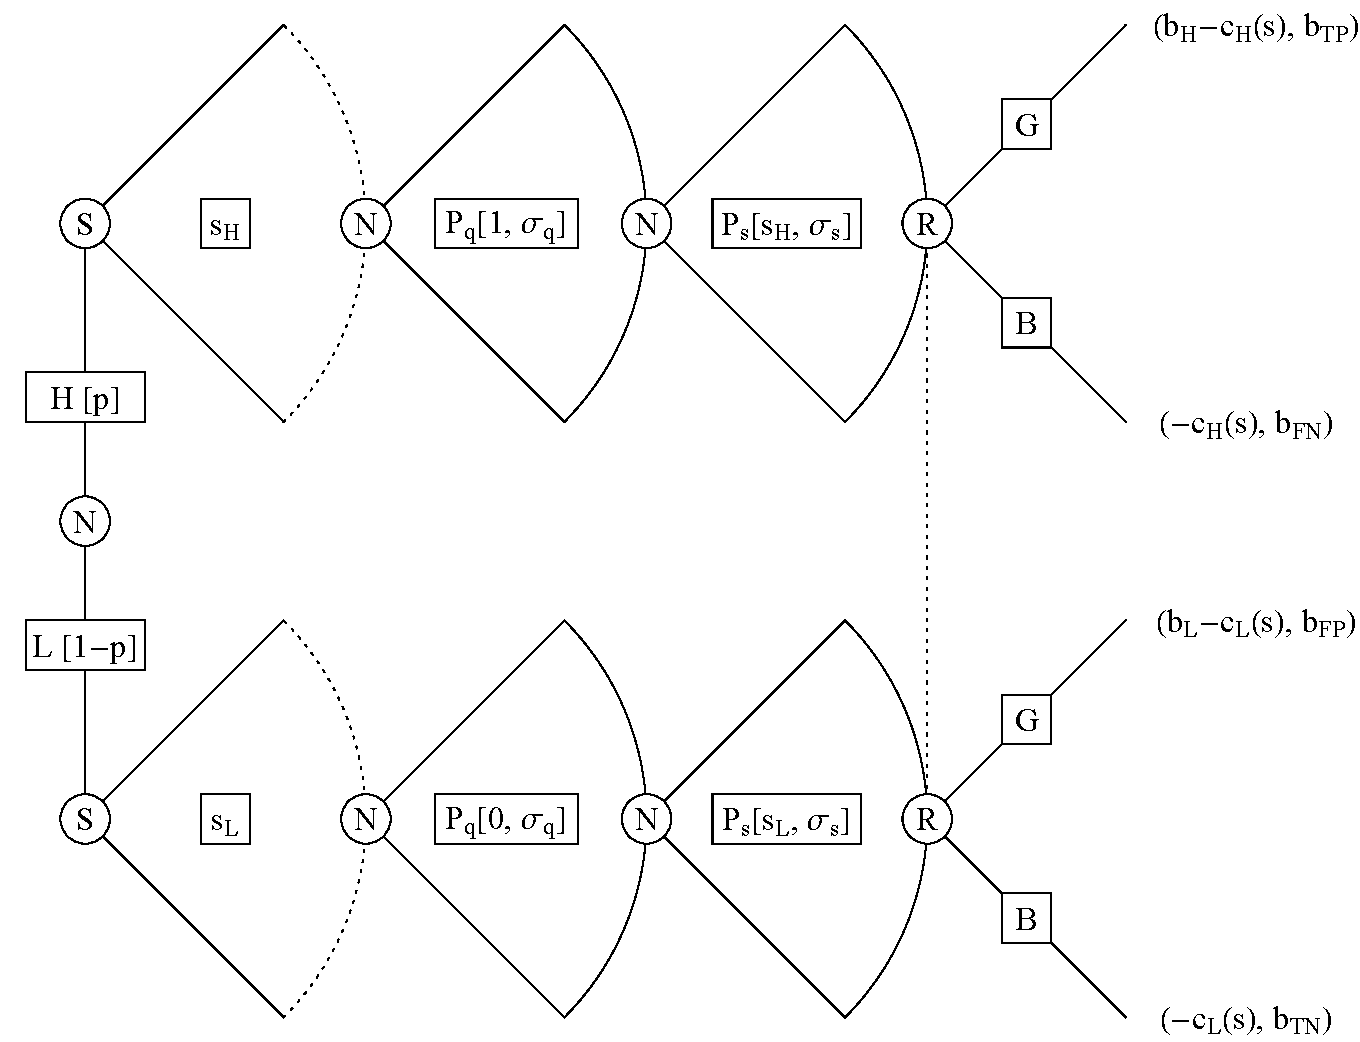
\includegraphics[scale=.58]{"Model 2/Figure 28.pdf}
\caption{Extensive form}
\label{fig:Model 2/Figure 28.pdf}
\end{center}
\end{figure}


\subsection{Receiver's Perspective}
\label{sec:CueandSignalDetectionModel/Receiver's Perspective}

We will follow a similar mathematical procedure to the one explained in section~\ref{sec:CueDetectionModelwithObservableAmplification/Receiver's Perspective}. In particular, we will turn the two-dimensional normal distribution into a one-dimensional version again.
\begin{figure}[!h]
\begin{center}
\leavevmode
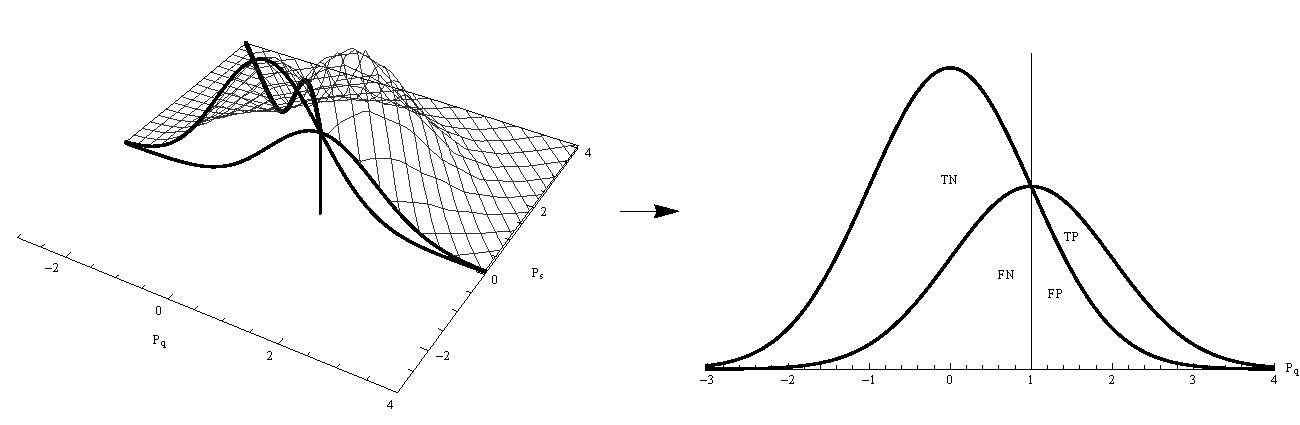
\includegraphics[scale=.61]{"Model 2/Figure 29.pdf}
\caption{Slicing the full model}
\label{fig:Model 2/Figure 29.pdf}
\end{center}
\end{figure}

The total payoff to the receiver is given in equation~\ref{eq:CueandSignalDetectionModel/PayoffR}.
\begin{equation}
\label{eq:CueandSignalDetectionModel/PayoffR}
\begin{array}{rcl}
P_{R}(R_{G}) &=& p \; b_{TP} \displaystyle \iint_{R_{G}} \mathcal{N}(P_{q}, P_{s}, q, s, \sigma_{q}, \sigma_{s}) \; dP_{q}dP_{s} +\\
&&p \; b_{FN} \displaystyle \iint_{R_{B}} \mathcal{N}(P_{q}, P_{s}, q, s, \sigma_{q}, \sigma_{s}) \; dP_{q}dP_{s} +\\
&&(1-p) \; b_{FP} \displaystyle \iint_{R_{G}} \mathcal{N}(P_{q}, P_{s}, q, s, \sigma_{q}, \sigma_{s}) \; dP_{q}dP_{s} +\\
&&(1-p) \; b_{TN} \displaystyle \iint_{R_{B}} \mathcal{N}(P_{q}, P_{s}, q, s, \sigma_{q}, \sigma_{s}) \; dP_{q}dP_{s}
\end{array}
\end{equation}

By not perfoming one of the two integrals, we obtain the sliced version of the receiver's payoff.
\begin{equation}
\label{eq:CueandSignalDetectionModel/SlicedPayoffR}
P_{R}(R_{G}) = \displaystyle \int \tilde{P}_{R}(\tilde{R}_{G}(P_{s})) \; dP_{s}
\end{equation}

Let us define $t(P_{s})=\partial \tilde{R}_{G}(P_{s})$ as the boundary of the region `good' and use differentiation under the integral sign to obtain equation~\ref{eq:CueandSignalDetectionModel/DifferentialPayoffR}.
\begin{equation}
\label{eq:CueandSignalDetectionModel/DifferentialPayoffR}
\frac{d}{dt}\tilde{P}_{R}(t)= \frac{(1-p) \; (b_{TP}-b_{FN})}{2 \pi \sigma_{q} \sigma_{s}} e^{-\frac{(0-t)^2}{2 \sigma_{q}^2}-\frac{(P_{s}-s_{L})^2}{2 \sigma_{s}^2}} - \frac{p \; (b_{TN}-b_{FP})}{2 \pi \sigma_{q} \sigma_{s}} e^{-\frac{(1-t)^2}{2 \sigma_{q}^2}-\frac{(P_{s}-s_{H})^2}{2 \sigma_{s}^2}}
\end{equation}

This will give us an expression for the optimal threshold $t$ as a function of the variable over which we had not performed the integration, $P_{s}$.
\begin{equation}
\label{eq:CueandSignalDetectionModel/Threshold}
t(P_{s})=\frac{(s_{H}^2-s_{L}^2)\sigma_{q}^{2}+\sigma_{s}^{2}}{2 \sigma_{s}^{2}}-\sigma_{q}^{2}\text{Log}[K]-(s_{H}-s_{L})\frac{\sigma_{q}^{2}}{\sigma_{s}^{2}} P_{s}
\end{equation}

This threshold function allows us to define the optimal region of perceptions for which the receiver does best to respond with $G$.
\begin{equation}
\label{eq:CueandSignalDetectionModel/RG}
R_{G} = \{P_{q}, P_{s} \in \mathbb{R}^{2} : P_{q}>t(P_{s})\}
\end{equation}


\subsection{Sender's Perspective}
\label{sec:CueandSignalDetectionModel/Sender's Perspective}

In a similar manner to section~\ref{sec:SignalDetectionModel/Sender's Perspective}, we can determine the payoff for the sender. Here, $b_{q} \in \{b_{H}, b_{L}\}$ and $c_{q} \in \{c_{H}, c_{L}\}$.
\begin{equation}
\label{eq:CueandSignalDetectionModel/PayoffS}
P_{S}(s) = b_{q} \displaystyle \iint_{R_{G}} \mathcal{N}(P_{q}, P_{s}, q, s, \sigma_{q}, \sigma_{s}) \; dP_{q}dP_{s}-c_{q}(s)
\end{equation}

Let us quickly examine the cost and benefit functions, to make an informed decision over the functional form of the cost function. As can be seen in figure~\ref{fig:Model 2/Figure 3132}, the marginal benefit of signalling starts off at zero, when signalling is zero. This has a quite simple explanation. In this model, the receiver obtains information concerning the quality of the sender from two sources; the quality cue and the level of signalling. If neither the high nor the low quality sender signals, the receiver assesses the quality of the sender using solely the quality cue. Consequently, there is no preference for signalling and no benefit in signalling to the sender. As the level of signalling increases, the receiver starts incorporating this information into its assessment of quality. Therefore, the marginal benefit of signalling increases.
\begin{figure}[h]
\begin{center}
\subfloat[Linear marginal cost]{\label{fig:Model 2/Figure 31.pdf}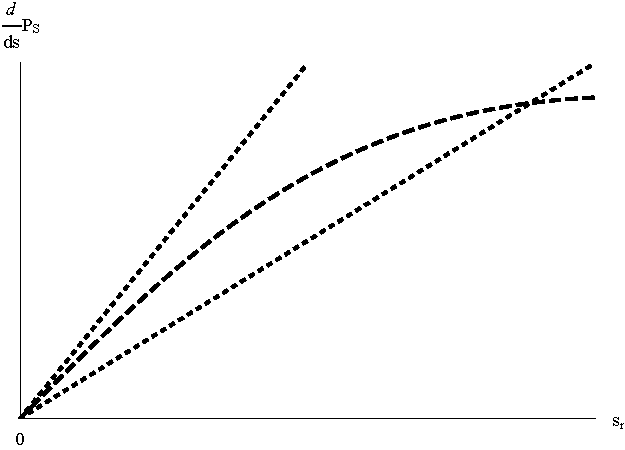
\includegraphics[scale=.6]{"Model 2/Figure 31.pdf}}
\hspace{8mm}
\subfloat[Quadratic marginal cost]{\label{fig:Model 2/Figure 32.pdf}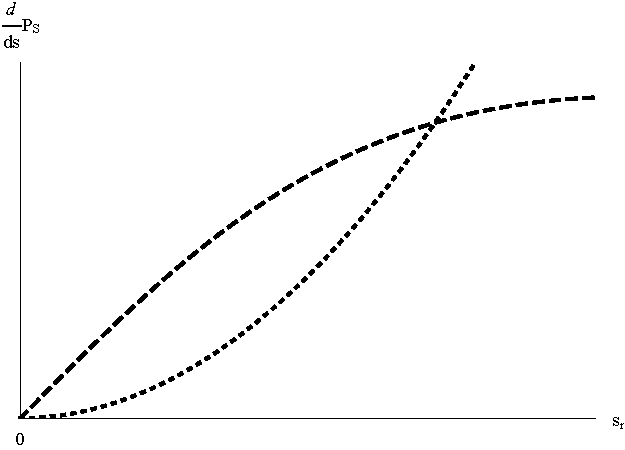
\includegraphics[scale=.6]{"Model 2/Figure 32.pdf}}
\caption{Cost (dotted) and benefit (dashed) functions}
\label{fig:Model 2/Figure 3132}
\end{center}
\end{figure}
 
If we were to choose a quadratically increasing cost function, meaning a linearly increasing marginal cost function, there would be some level of cost for which it does not pay the sender to signal. This can be seen in figure~\ref{fig:Model 2/Figure 31.pdf}. This upper limit on the cost has a completely arbitrary value and provides little realism to our model. In fact, it only complicates our model, making the final results harder to interpret. If we were to choose a cost function which increases cubicly, this problem does not arise. The results of our model would be much smoother and more easily interpreted. No matter what cost, the sender would adopt at least some level of signalling. We shall, therefore, choose a simple cubicly increasing cost function, as given in equation~\ref{eq:CueandSignalDetectionModel/CostFunction}.
\begin{equation}
\label{eq:CueandSignalDetectionModel/CostFunction}
c_{q}(s)=c_{q} \, s^{3}
\end{equation}

Let us continue with our aim of calculating the marginal payoff of signalling. Equation~\ref{eq:CueandSignalDetectionModel/PayoffS}, again, does not have a closed form. However, we can do one of the two integrals, leaving $P_{s}$ as a variable.
\begin{equation}
\label{eq:CueandSignalDetectionModel/SlicedPayoffS}
P_{S}(s) = \displaystyle \int \tilde{P}_{S}(s) \; dP_{s}-c_{q}(s)
\end{equation}

This will allow us to perform the same trick as in section~\ref{sec:CueDetectionModelwithObservableAmplification/Sender's Perspective}, commuting the derivative operator with the integral. As seen in equation~\ref{eq:CueandSignalDetectionModel/DifferentialPayoffS}, this allows us to obtain a closed form solution for the marginal payoff of signalling. Here, $\alpha$ and $\beta$ are defined such that $t(P_{s})=\alpha+\beta \, P_{s}$.
\begin{equation}
\label{eq:CueandSignalDetectionModel/DifferentialPayoffS}
\begin{array}{rcl}
\frac{d}{ds} P_{S}(s) &=& \displaystyle \int \frac{d}{ds} \tilde{P}_{S}(s) \; dP_{s} - \frac{d}{ds} c_{q}(s)\\[3mm]
&=& \displaystyle \frac{b \; \beta}{\sqrt{2 \pi} \sqrt{\sigma_{q}^{2} + \beta^2 \, \sigma_{s}^{2}}} \; e^{-\frac{(q-\alpha-s \beta)^{2}}{2(\sigma_{q}^{2}+\beta^{2} \sigma_{s}^{2})}} - 3 \, c_{q} \, s^2
\end{array}
\end{equation}


\subsection{Equilibria}
\label{sec:CueandSignalDetectionModel/Equilibria}

We can find an analytical expression for the ratio between the level of signalling of the high quality sender and the low quality sender. Following the discussion of the relative costs and benefits of signalling in section~\ref{sec:SignalDetectionModel/Equilibria}, we can again use the parameter $r_{c}$. This time, the ratio between the level of signalling, however, contains a square root. This comes from our choice of a quadratic marginal cost function.
\begin{equation}
\label{eq:CueandSignalDetectionModel/Ratio}
r=\sqrt{r_{c} K}
\end{equation}

This ratio has the interesting property that it can exceed $1$. This might suggest that the low quality sender would signal at a level higher than the high quality sender, even when its costs are higher. However, this would not make sense, as it is in the low quality sender's interest to resemble a high quality sender as best as possible. The low quality sender wants to do what the high quality sender does, because that way it might be mistaken for a high quality sender and get response $G$ from the receiver.
\begin{equation}
\label{eq:CueandSignalDetectionModel/Zone}
K <\frac{1}{r_{c}}
\end{equation}

Therefore, it must be concluded that, if ratio $r$ exceeds $1$, the only possibility is that the level of signalling is zero. This reduces to the condition for signalling in equation~\ref{eq:CueandSignalDetectionModel/Zone}, which is shown graphically in figure~\ref{fig:Model 2/Figure 30.pdf}.

\begin{figure}[h]
\begin{center}
\leavevmode
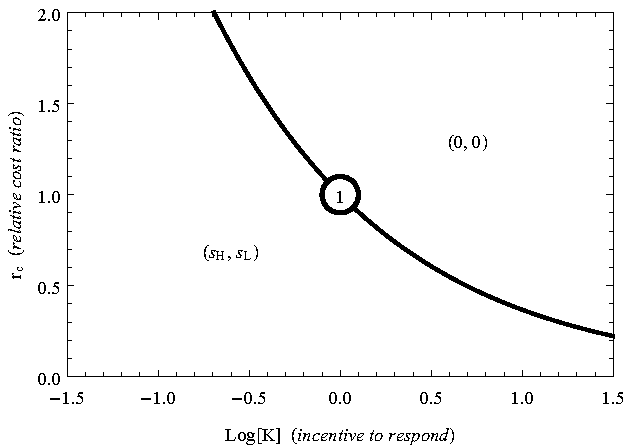
\includegraphics[scale=.9]{"Model 2/Figure 30.pdf}
\caption{Equilibria}
\label{fig:Model 2/Figure 30.pdf}
\end{center}
\end{figure}

Another way to look at the condition in equation~\ref{eq:CueandSignalDetectionModel/Zone} is that, when $K$ is high, the benefit of signalling is such that it allows low quality signallers to `keep up' with high quality ones. No matter what level of signalling the high quality sender chooses, the low quality sender will choose, and will be able to choose, that same level. There is, therefore, no benefit from signalling for the high quality sender, who will choose not to signal at all. Figure~\ref{fig:Model 2/Figure 30.pdf} shows these two zones in parameter-space.

Furthermore, it can be concluded that signalling is far more stable if there is a secondary quality cue present. This is easily seen by comparing the ranges of parameters for which signalling occurs in figure~\ref{fig:Model 2/Figure 30.pdf} with figure~\ref{fig:Model 2/Figure 23.pdf} of our previous, simpler model. In the previous model, a Log[$K$] different from zero led to a rapid decrease in the benefit of signalling. This quickly caused the signalling equilibrium to disappear, as seen in figure~\ref{fig:Model 2/Figure 202122}. In this model, non-zero values of Log[$K$] can still lead the instability of the signalling equilibrium. Fortunately, it only happens for extremely high or extremely low values of Log[$K$], or when $\sigma_{q}$ is so high that the current model basically reduces to the previous model with the quality cue. Therefore, the addition of a quality cue makes handicap signalling more stable. More precisely, a low value of $\sigma_{q}$ results in the stability of the signalling equilibrium over a wider range of parameter-values. This is a key finding of this model.

What is even more interesting is that signalling is possible even when the cost to the high quality sender is higher than the cost to the low quality sender. This only arises when Log[$K$] is very low. For a low Log[$K$], the threshold between $R_{B}$ and $R_{G}$ is set very high, meaning the receiver only responds with $G$ when the perceived level of quality is high. This comes as a disadvantage to the low quality sender, who, despite its relatively low cost of signalling, will not feel an incentive to signal strongly. The marginal benefit of signalling is determined by the height of the normal distribution at the threshold. Therefore, in this case, the benefit of signalling is far larger for the high quality sender than it is for the low quality sender. Even though the cost of signalling to the high quality sender is substantial, it will signal at a higher level than the low quality sender. In our model of handicap signalling with an additional quality cue, it can be seen that the stability of signalling does not necessarily need differential costs, but that differential benefits arise naturally. This is another key finding of this model.

Assuming that the signalling equilibrium is stable, we can use equation~\ref{eq:CueandSignalDetectionModel/DifferentialPayoffS} to determine the level at which each type of sender will signal as a function of the costs. Figure~\ref{fig:Model 2/Figure 3334} shows these levels for the high and the low quality sender, having set $b_{H}=b_{L}=1$.
\begin{figure}[h]
\captionsetup{width=380pt}
\begin{center}
\subfloat[Level of signalling for the high quality sender]{\label{fig:Model 2/Figure 33.pdf}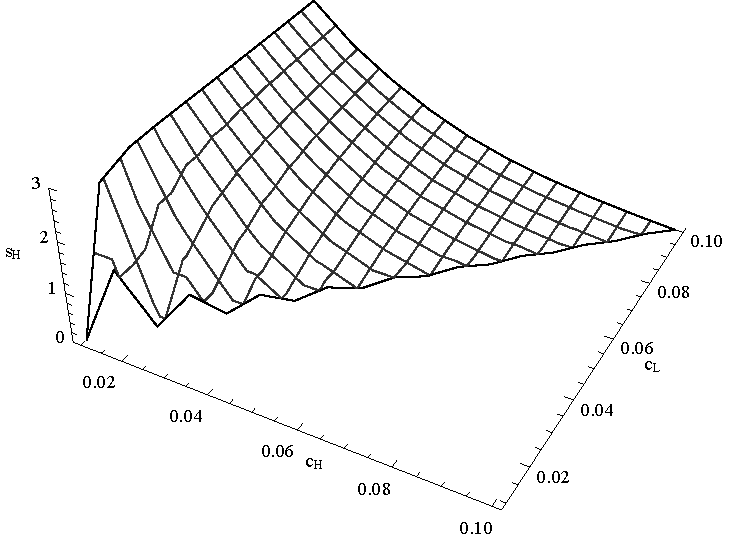
\includegraphics[scale=.6]{"Model 2/Figure 33.pdf}}
\hspace{4mm}
\subfloat[Level of signalling for the low quality sender]{\label{fig:Model 2/Figure 34.pdf}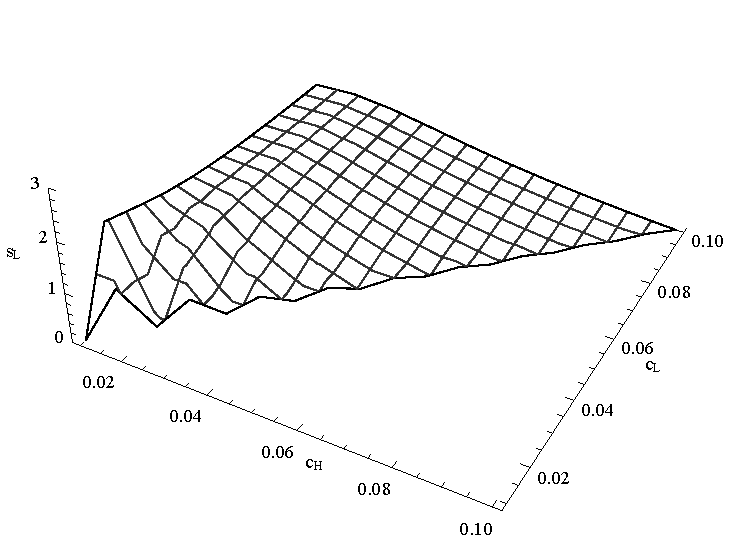
\includegraphics[scale=.6]{"Model 2/Figure 34.pdf}}
\caption{Levels of signalling as a function of the costs with Log[$K$]$=0$, $\sigma_{q}=1$ and $\sigma_{s}=1$, keeping $c_{H}<c_{L}$.}
\label{fig:Model 2/Figure 3334}
\end{center}
\end{figure}

\newpage

It may also be interesting to plot this same information in a two-dimensional figure. In this case, we can include the information content of the signal as well. This is done in figure~\ref{fig:Model 2/Figure 35.pdf}.
\begin{figure}[h]
\captionsetup{width=300pt}
\begin{center}
\leavevmode
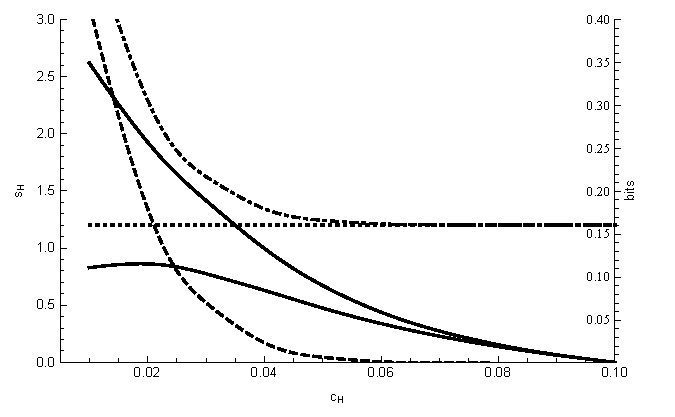
\includegraphics[scale=1.1]{"Model 2/Figure 35.pdf}
\caption{Level of signalling for the high quality sender (thick) and low quality sender (thick) as a function of the relative cost, as well as the information content of the quality cue (dotted), the signal (dashed) and both messages combined (dot-dashed), when $c_{L}=0.10$.}
\label{fig:Model 2/Figure 35.pdf}
\end{center}
\end{figure}


\subsection{Example}
\label{sec:CueandSignalDetectionModel/Example}

The begging displays of young chicks, soliciting for food to their parents, can be explained theoretically as a form of handicap signalling~\cite{Godfray1991}. There is a large variety of species whose young show begging displays~\cite{Kilner1997}. One example is of the canary \textit{Serinus canaria}, whose parents respond to calling behaviours of the chicks by feeding louder chicks more~\cite{Kilner1995}. One way in which the honesty of these begging calls is maintained is through energy costs. In an experiment, a higher begging intensity led to mass loss as a result of metabolic expenditure. It has also been shown that excessive begging retarded growth. Limiting growth might be interpreted as a fitness cost, as daily mass gain correlates with the likelihood of survival to independence~\cite{Kilner2001}. It has been shown that the canary parents are able to respond to many cues besides the begging display when allocating food~\cite{Kilner1995}. It is reasonable to assume the parents are able to assess their offspring's need for food in a more direct manner. For example, by remembering the amount of food it provided to each chick in previous feeding-sessions, it can estimate how needy a chick truly is. This assessment, relying on memory, is obviously error-prone. However, the current model has shown that even an error-prone cue can have a large impact by making the signalling mechanism more stable.

\newpage\clearpage


\section{Discussion}
\label{sec:Part 3/Discussion}
\subsection{A More Realistic Model}
\label{sec:A More Realistic Model}

The model of section~\ref{sec:Cue Detection Model with Observable Amplification} shows that, when an amplifying display is observable to females, the display becomes attractive. This is because high quality males will choose to amplify their cue, making amplification a thing high quality males do. Consequently, females learn to use this information in their assessment of males, requiring some level of amplification before accepting a mate. The result of our model is that low quality males, who initially prefer to conceal their bad quality, are forced to amplify as well.

Figure~\ref{fig:Model 2/Figure 18.pdf} illustrates the model best. It shows that females will accept a male when its perceived quality and its perceived level of amplification are above a particular threshold. When females are cautious, associated with a smaller value for $K$, the region `good' becomes small. The threshold-line can then be seen to retreat to the upper-right corner of figure~\ref{fig:Model 2/Figure 18.pdf}. If this figure was divided into quadrants, only perceptions within the upper-right quadrant would lead to the favourable response $G$. This is equivalent to the $GBBB$~strategy of the model in section~\ref{sec:Cue Game with Observable Amplification}, which is also an equilibrium-strategy for the receiver when $p$ is low. Contrarily, when females are lenient in their assessment of males, the threshold-line moves to lower values, accepting more males.

We can, therefore, see that the predicted behaviours of the models in part~\ref{sec:Amplifiers and Signal Detection Theory} agree with those of part~\ref{sec:The Transition to Signalling through Amplification}. However, there are two advantages of the models of part~\ref{sec:Amplifiers and Signal Detection Theory}. First of all, the mathematics of the previous sections is relatively easy and visualising the optimal behaviour of the sender and the receiver is straightforward. Secondly, the assumption that the perception of quality and amplification moves on a continuous scale is more realistic than the binary choices of part~\ref{sec:The Transition to Signalling through Amplification}. As the examples in the previous sections should have made clear, both quality and amplification can take on a whole range of values and the notion that a receiver sets a threshold level to distinguish different types of senders makes intuitive sense.

It should be clear that the language of sexual selection makes the discussions of these models easier, but, as many examples in this thesis have shown, the models are general enough to be applied to any type of animal communication. In fact, as mentioned in section~\ref{sec:Amplifiers in Economics}, the models may even find application in economics, where the concept of information plays a vital role. The notion of amplifiers as a method of reducing \mbox{perception-errors}, as well as the new model for handicap signalling in section~\ref{sec:Cue and Signal Detection Model}, may illuminate specific economic behaviour.

The advantages of the continuous version of our model became even more evident when examining handicap signalling. It turned out that the framework developed in section~\ref{sec:Cue Detection Model with Observable Amplification} allowed for a very easy re-interpretation. The final model shows that handicap signalling can be stable over a wide range of parameter-values, when it is combined with the perception of a quality cue. A suggestion of such a multiple-message model has been given in section~\ref{sec:CueandSignalDetectionModel/Example}. Hopefully this thesis provides a further incentive to empiricists to explore evidence for the use of multiple messages in animal communication.

\newpage\clearpage


\part{Patterns as an Example of Amplifiers}
\label{sec:Patterns as an Example of Amplifiers}
\addtocontents{toc}{\protect\vspace{1mm}}

\newpage\clearpage


\section{Introduction}
\label{sec:Part 4/Introduction}
\subsection{Patterns and Visual Perception}
\label{sec:Patterns and Visual Perception}

The original idea of amplification is based on verbal arguments by Zahavi~\cite{Zahavi1978}. In his article on decorative patterns, Zahavi presented a simple example of an amplifying dot in the center of a circle. He supposed that there was a set of circles which where all slightly asymmetric. The level of symmetry of a circle would represent its `quality'. The perception of the symmetry may not be perfect, however, and judging which of two circles is of `better quality' can be hard. A dot in the center of these circles would help with the assessment of symmetry and reduce errors in perception. This dot satisfies Hasson's definition of an amplifier.

The example by Zahavi is useful because of its simplicity. The assessment of symmetry is important in biology and this example is stripped to its core, retaining only the relevant features of quality assessment and error in perception~\cite{Moller1997, Johnstone1994}. As such, it might be interesting to see whether Zahavi's original suggestion holds up in an experiment. Do people actually find it easier to assess the symmetry of a circle when there is a dot present?

This final part of the thesis serves to illustrate the concept of an amplifier by means of a simple experiment. It will show that a very basic pattern can have an influence over the perception of quality. A similar experiment has already shown that patterns can, indeed, improve the perception of other characteristics. In section~\ref{sec:CueDetectionModelwithObservableAmplification/Example}, we discussed female pipefish who have a cross-wise striped pattern along their body~\cite{Berglund2000}. In an study with students, it has been shown that this pattern can facilitate the assessment of width of a rectangle.


\subsection{Circles with Dots}
\label{sec:Circles with Dots}

To test Zahavi's hypothesis that a dot in the center of a circle helps with the assessment of the symmetry of that circle by reducing errors in perception, a short experiment is performed. In this experiment, participants are presented with two circles. Each circle is slightly asymmetric, with one more so than the other. The task is to select the most symmetric circle. This is a two-alternative forced choice (`2AFC') task. When there is a dot present in the center of the circles, will people find it easier to assess the symmetry?
\begin{figure}[!h]
\begin{center}
\captionsetup[subfigure]{width=30mm}
\subfloat[Most symmetric without a dot]{\label{fig:Experiment 1/Figure 1.pdf}\includegraphics[scale=.24]{"Experiment 1/Figure 1.pdf}}
\hspace{6mm}
\subfloat[Least symmetric without a dot]{\label{fig:Experiment 1/Figure 2.pdf}\includegraphics[scale=.24]{"Experiment 1/Figure 2.pdf}}
\hspace{6mm}
\subfloat[Most symmetric with a dot]{\label{fig:Experiment 1/Figure 3.pdf}\includegraphics[scale=.24]{"Experiment 1/Figure 3.pdf}}
\hspace{6mm}
\subfloat[Least symmetric with a dot]{\label{fig:Experiment 1/Figure 4.pdf}\includegraphics[scale=.24]{"Experiment 1/Figure 4.pdf}}
\caption{The four possible circles with and without a dot}
\label{fig:Experiment 1/Figure 1234}
\end{center}
\end{figure}

\newpage\clearpage


\section{Experimental Setup}
\label{sec:Experimental Setup}
\subsection{Methods}
\label{sec:Methods}

The experiment is designed using the computer programme \textit{Adobe Flash}. In this Flash application, two circles are drawn. The first has a width of 98 pixels and a height of 102 pixels. The second circle has a width of 96 pixels and a height of 104 pixels. The second circle is, therefore, slightly more asymmetric, with the total area of the circles kept, more or less, the same.

The Flash application is designed such that participants first read a general description of the experiment and, then, select their gender and their age-group. The following instructions inform them that they will be shown pairs of circles and should select the most symmetric circle using the arrow-keys on their keyboard. They are told to be as fast as possible in their assessment of the symmetry. Their answer is recorded, as well as their reaction time at a framerate of 24 fps. There is a 5 second maximum per trial and a missing value is recorded if a participant does not answer in time. Five second is more than enough to make a decision and this restriction is mostly meant to check whether participants are paying careful attention to the experiment.

In each trial, the participants see either a pair of circles without a dot or a pair with a dot. One circle is presented left-of-center while the other is right-of-center. One of these circles is the more symmetric type, while the other the more asymmetric. Due to the asymmetry, a main axis can be defined within each circle. To avoid this influencing the results, the pairs of circles are rotated at random between each trial. The circles are also moved vertically between trials, alternating between just above or just below the center-line. This is to avoid participants assessing the symmetry of a circle by comparing it to the previous circle of the previous trial in that same position.

Considering the two possible pairs of circles, with and without a dot, the two possible positions of the most symmetric one, left or right, and the two possible vertical positions, above or below the center-line, there are 8 different possible pairs of circles. The order in which these 8 pairs are presented to participants is randomised. Three subsets of 8 pairs are grouped together to form a set. The experiment contains four sets and participants are given 10 second breaks in between each set. The first set was considered a practice set and the results were not considered in the final analysis.

In total, 103 people participated in this experiment. They were recruited using the crowdsourcing Internet marketplace \textit{Amazon Mechanical Turk}. Mechanical Turk `workers' were told the experiment lasted about 5 minutes and that they would receive 0.50~USD for their participation. They were given a link to another website which displayed the Flash application and which stored the data from all participants.


\subsection{Statistical Analyses}
\label{sec:Statistical Analyses}

The hypothesis, orginially expressed by Zahavi, was that the dot in the center of the circle serves as an amplifier by allowing for an easier assessment of the symmetry of that circle~\cite{Zahavi1978}. More precisely, participants should, on average, have a higher proportion of correct answers, $P_{c}$, when presented with pairs of circles with a dot than for pairs without a dot. They should also be faster is their assessment of symmetry and, thus, have a lower average reaction time, $\mu_{RT}$. Reaction times were recorded for all trials, but only those trials in which the participant answered correctly were taking into consideration when calculating the average reaction time. Finally, it may be suggested that the variance in the reaction time, $\sigma_{RT}^{2}$, should be lower for the amplified circles.

In psychophysics, the field which concerns itself with human perception, there are many models which try to understand human decision making. One of the main purposes of some of these models is to combine information from $P_{c}$, $\mu_{RT}$ and $\sigma_{RT}^{2}$ to create a single variable which represents the ease with which a decision is made. One well-documented model is the diffusion model in which the drift rate, $\nu$, is the variable which represents how fast someone `drifts' towards the correct answer. The model by Wagenmakers et al. is a simplified version of such a diffusion model and should be enough to help us create a single variable representing the process in the assessment of symmetry for our circles~\cite{Wagenmakers2007}.

In their article, the authors discuss three assumptions which need to be satisfied before any conclusion can be drawn from the results. The first assumption is that the distribution in reaction times should show positive skew, $\gamma_{1}$, and that the skew should be bigger for the more difficult task. Let us call the circles without a dot the `concealed' circles and the ones with a dot the `amplified' ones. In our experiment, $\gamma_{1}\text{[Concealed]} = 0.764$ and $\gamma_{1}\text{[Amplified]} = 0.878$. The assumption of positive skew holds, but the relative difference between the circles with a dot and those without suggest that, perhaps, the supposedly `amplified' circle actually belongs to the more difficult task. The second assumption is that the distribution for the reaction times has the same shape for correct and error responses. This means there should be no correlation, $\rho$, between the recorded reaction time and whether the answer was correct. In our experiment, this correlation was negligibly small; $\rho \text{[Correct, Time]} = 0.0783$. Finally, the third assumption is that there is no a priori bias in selecting either one of the two stimuli. As the most symmetric circle was found on the left side of the screen equally often as on the right side of the screen, this assumption is met too.

In the simplified version of the diffusion model, there is an analytical expression for the drift rate. Taking $s = 0.1$, the $P_{c}$ and $\sigma_{RT}^{2}$ of each participant can be used to determine their drift rate for circles with and without a dot.
\begin{equation}
\label{eq:DriftRate}
\nu = \text{sign} \left[ P_{c} - \frac{1}{2} \right] s \left( \frac{\text{logit}[P_{c}] (P_{c}^{2} \, \text{logit}[P_{c}] - P_{c} \, \text{logit}[P_{c}] + P_{c} - \frac{1}{2})}{\sigma_{RT}^{2}} \right)^{\frac{1}{4}}
\end{equation}

Out of the 103 participants of this experiment, a simple check of the data showed several people did not follow the instructions correctly. These participants either had many missing values, a strong bias towards one side (for example, always clicking the right arrow-key, regardless of the circle) or impossibly short reaction times. These participants were excluded from the analysis, leaving 90 data entries.


\subsection{Results}
\label{sec:Results}

The results of our experiment are summarised in table~\ref{tab:ResultsExperiment}. This table lists the value for the proportion of correct answers, mean reaction time, variance in reaction time and the drift rate. It also gives the difference between the means and the associated paired t-test. Due to the fact that the distributions were not always normal, a non-parametric test was necessary. The Wilcoxon signed-rank test allows for a comparison of non-normally distributed paired data.

\vspace{4mm}

\begin{table}[h]
\begin{center}
\begin{tabular}{r|ccccc}
&Concealed&Amplified&Difference&t-test&Wilcoxon test\\
\hline
$P_{c}$&0.791&0.761&-0.0294&0.0166&0.0260\\
$\mu_{RT}$&20.4&20.7&0.179&0.451&0.359\\
$\sigma_{RT}^{2}$&46.2&52.1&5.92&0.656&0.570\\
$\nu$&0.0247&0.0216&-0.00307&0.0220&0.0292
\end{tabular}
\end{center}
\captionsetup{width=100mm}
\caption{The proportion of correct answers, mean reaction time, variance in reaction time and drift rate.}
\label{tab:ResultsExperiment}
\end{table}

\vspace{6mm}

The proportion of correct answers was significantly greater ($p=0.0260$) for the supposedly `concealed' type of circle.
\begin{figure}[h]
\begin{center}
\subfloat[Histogram]{\label{fig:Experiment 1/Figure 5.pdf}\includegraphics[scale=.65]{"Experiment 1/Figure 5.pdf}}
\hspace{4mm}
\subfloat[Box plot]{\label{fig:Experiment 1/Figure 6.pdf}\includegraphics[scale=.65]{"Experiment 1/Figure 6.pdf}}
\caption{Histogram and box plot of the proportion of correct answers}
\label{fig:Experiment 1/Figure 56}
\end{center}
\end{figure}

\newpage

Participants were not any faster in making their decisions when presented with a pair of circles without a dot ($p=0.359$). The variance in these reaction times was also the same.\begin{figure}[h]
\begin{center}
\subfloat[Histogram]{\label{fig:Experiment 1/Figure 7.pdf}\includegraphics[scale=.65]{"Experiment 1/Figure 7.pdf}}
\hspace{4mm}
\subfloat[Box plot]{\label{fig:Experiment 1/Figure 8.pdf}\includegraphics[scale=.65]{"Experiment 1/Figure 8.pdf}}
\caption{Histogram and box plot of the mean reaction time}
\label{fig:Experiment 1/Figure 78}
\end{center}
\end{figure}

The drift rate, which combines these measures into a single variable, showed ($p=0.0292$) that the dot in the center of the circles did not make it easier to assess the symmetry of that circle. In fact, it made it significantly harder. Our initial hypothesis is rejected.
\begin{figure}[h]
\begin{center}
\subfloat[Histogram]{\label{fig:Experiment 1/Figure 9.pdf}\includegraphics[scale=.65]{"Experiment 1/Figure 9.pdf}}
\hspace{4mm}
\subfloat[Box plot]{\label{fig:Experiment 1/Figure 10.pdf}\includegraphics[scale=.65]{"Experiment 1/Figure 10.pdf}}
\caption{Histogram and box plot of the drift rate}
\label{fig:Experiment 1/Figure 910}
\end{center}
\end{figure}

\newpage\clearpage


\section{Discussion}
\label{sec:Part1/Conclusion}
\subsection{Possible Explanations}
\label{sec:Possible Explanations}

Our hypothesis that a dot in the center of a circle would function as an amplifier of the perception of symmetry was false. One possible reason for this is that the additional stimulus of the dot surprises and confuses people. It may take people longer to fully observe all features of the image they are presented with, giving more time for errors to emerge. Another possibility is that, when asked to respond as fast as possible, people gaze more at the outer sides of the image and less at the center. In this case, too, the dot has no benefit to the assessment of symmetry.

\subsection{Example of a Concealer}
\label{sec:Example of a Concealer}

Given that the difference in the proportion of correct answers was significant for the `concealed' and `amplified' circles, it can be concluded that the pattern did have an effect on symmetry perception. The direction of the effect, however, was opposite to the one hypothesised. This suggests that the circles with a dot are actually the concealed version, while the ones without the dot are amplified. As such, we might be able to conclude the dot functions as a concealer. This shows that patterns can, indeed, effect the error in perception of a display. Patterns are not the only type of amplifying or concealing display. There may be many types, including colours, contour lines and even behaviours.

Although the literature on amplifiers is not vast, there are some tentative examples of displays functioning as amplifiers of other displays. We have seen some in the `Example' sections of part~\ref{sec:The Transition to Signalling through Amplification} and part~\ref{sec:Amplifiers and Signal Detection Theory}. There are, so far, no clear examples of concealers. Some arguments suggest concealers are less likely to evolve as they improve the mating success of low quality animals, while amplifiers rely on their benefit to high quality ones~\cite{Hasson1992}. Nonetheless, there is a mathematical symmetry between concealers and amplifiers, and concealers may play a role in many communication systems in nature. Hopefully this experiment provides further incentive to empiricists to explore evidence for the use of concealing displays in animal communication.

\newpage \clearpage
\addtocontents{toc}{\protect\vspace{4mm}}

\bookmarksetup{startatroot}
\phantomsection
\label{sec:Bibliography}
\addcontentsline{toc}{section}{Bibliography}
\renewcommand{\refname}{Bibliography}
\bibliographystyle{acm}
\bibliography{Bibliography}


\newpage\clearpage
\addtocontents{toc}{\protect\vspace{4mm}}

\pdfbookmark{Appendix}{Appendix}
\appendix

\section{Regions for Costly Amplification}
\label{sec:Regions for Costly Amplification}
\subsection{Cue Game with Unconditional Amplification}
\label{sec:Appendix/Cue Game with Unconditional Amplification}

In this appendix, we will look at costly amplification. Throughout, we assume $c_{H} \leq c_{L}$, keeping in mind that a costly amplifier is not necessarily the same as a handicap amplifier if there is no direct preference for the display. We will determine the expected payoffs, the new regions of parameter-space, the best responses and the new equilibria. Luckily, compared to the cost-free version of unconditional amplification, discussed in section~\ref{sec:Cue Game with Unconditional Amplification}, the expected payoffs only change for the sender. Table~\ref{tab:Appendix/Cue Game with Unconditional Amplification/ConditionalPayoffsS} lists the new expected payoffs.

\begin{table}[h]
\begin{center}
\begin{tabular}{lcccccrcc}
$P_{S}(A|GG)$ & $=$ & $p(1-c_{H})+(1-p)(1-c_{L})$ & $>$ & $1$ & $=$ & $P_{S}(K|GG)$ & for & no value\\
$P_{S}(A|GB)$ & $=$ & & & & $=$ & $P_{S}(K|GB)$ & \multirow{3}{*}{for} & \multirow{3}{*}{$f_{9}<p$}
\vspace{-1mm}\\
\multicolumn{3}{l}{$p(1-e_{1})(1-c_{H})+p(e_{1})(-c_{H})+$} & & \multicolumn{3}{c}{$p(1-e_{2})+$} 
\vspace{-1mm}\\
\multicolumn{3}{r}{$(1-p)(e_{1})(1-c_{L})+(1-p)(1-e_{1})(-c_{L})$} & $>$ & \multicolumn{3}{l}{$(1-p)(e_{2})$} 
\vspace{1mm}\\
$P_{S}(A|BB)$ & $=$ & $p(-c_{H})+(1-p)(-c_{L})$ & $>$ & $0$ & = & $P_{S}(K|BB)$ & for & no value
\end{tabular}
\end{center}
\caption{Sender's expected payoffs}
\label{tab:Appendix/Cue Game with Unconditional Amplification/ConditionalPayoffsS}
\end{table}

\vspace{6mm}

Equation~\ref{eq:f9} describes the boundary of the two regions of parameter-space.
\begin{equation}
\label{eq:f9}
f_{9}(e_{1},e_{2},c_{H},c_{L})=\frac{(e_{2}-e_{1})+c_{L}}{2(e_{2}-e_{1})+(c_{L}-c_{H})}
\end{equation}

Let us try to interpret this equation, by looking closely at the expected payoff under $GB$. Rearranging $f_{9}<p$, we obtain the inequality of equation~\ref{eq:Inequality}.
\begin{equation}
\label{eq:Inequality}
p c_{H}+(1-p)c_{L}<p(e_{2}-e_{1})-(1-p)(e_{2}-e_{1})
\end{equation}

The left-hand-side is the expected cost of amplification, a weighted average over the two, possibly different, costs of amplifying to the high and the low quality sender. The right-hand-side of the equation describes the benefit of amplifying. The benefit consists of two parts, a positive effect of size $e_{2}-e_{1}$ on the $p$ proportion of senders who are of high quality and a negative effect on the $1-p$ proportion low quality senders. Clearly, this condition merely states that a sender should only amplify if the benefit of doing so is greater than the cost.

The regions of parameter-space change according to table~\ref{tab:Appendix/Cue Game with Unconditional Amplification/RegionS}.

\begin{table}[h]
\begin{center}
\begin{tabular}{lc}
Region S1: & $p<f_{9}$\\
Region S2: & $f_{9}<p$
\end{tabular}
\end{center}
\caption{Sender's regions}
\label{tab:Appendix/Cue Game with Unconditional Amplification/RegionS}
\end{table}

\newpage

The best responses of the sender change according to table~\ref{tab:Appendix/Cue Game with Unconditional Amplification/BestResponseS}.

\begin{table}[h]
\begin{center}
\begin{tabular}{lccc}
 & GG & GB & BB\\
Region S1: & K & K & K\\
Region S2: & K & A & K
\end{tabular}
\end{center}
\caption{Sender's best response}
\label{tab:Appendix/Cue Game with Unconditional Amplification/BestResponseS}
\end{table}

The equilibria of this costly model change according to table~\ref{tab:Appendix/Cue Game with Unconditional Amplification/Equilibria}. Some regions which in the cost-free version did not exist now do appear.

\begin{table}[h]
\begin{center}
\begin{tabular}{lcc}
 & Region S1 & Region S2\\
Region R1: & (K, BB) & x\\
Region R2: & (K, BB) & x\\
Region R3: & (K, GB) & (A, GB)\\
Region R4: & (K, GG) & (A, GB) \& (K, GG)\\
Region R5: & (K, GG) & (K, GG)
\end{tabular}
\end{center}
\caption{Equilibria}
\label{tab:Appendix/Cue Game with Unconditional Amplification/Equilibria}
\end{table}

\newpage \clearpage


\subsection{Cue Game with Conditional Amplification}
\label{sec:Appendix/Cue Game with Conditional Amplification}

Table~\ref{tab:Appendix/Cue Game with Conditional Amplification/ConditionalPayoffsS} lists the new expected payoffs for a model of costly conditional amplification.

\begin{table}[h]
\setlength{\tabcolsep}{.3em}
\begin{center}
\begin{tabular}{lccccrrcc}
$P_{S}(A|H_{S},GG)$ & $=$ & $\frac{p(1-e_{4})(1-c_{H})+(1-p)(e_{4})(1-c_{L})}{p(1-e_{4})+(1-p)(e_{4})}$ & $>$ & $1$ & $=$ & $P_{S}(K|H_{S},GG)$ & for & no value\\
$P_{S}(A|L_{S},GG)$ & $=$ & $\frac{p(e_{4})(1-c_{H})+(1-p)(1-e_{4})(1-c_{L})}{p(e_{4})+(1-p)(1-e_{4})}$ & $>$ & $1$ & $=$ & $P_{S}(K|L_{S},GG)$ & for & no value\\
$P_{S}(A|H_{S},GB)$ & $=$ & \multicolumn{7}{l}{$\frac{p(1-e_{4})(1-e_{1})(1-c_{H})+p(1-e_{4})(e_{1})(-c_{H})+(1-p)(e_{4})(e_{1})(1-c_{L})+(1-p)(e_{4})(1-e_{1})(-c_{L})}{p(1-e_{4})+(1-p)(e_{4})}$}
\vspace{1mm}\\
\multicolumn{5}{r}{$> \frac{p(1-e_{4})(1-e_{2})+(1-p)(e_{4})(e_{2})}{p(1-e_{4})+(1-p)(e_{4})}$} & $=$ & $P_{S}(K|H_{S},GB)$ & for & $f_{10}<p$
\vspace{2mm}\\
$P_{S}(A|L_{S},GB)$ & $=$ & \multicolumn{7}{l}{$\frac{p(e_{4})(1-e_{1})(1-c_{H})+p(e_{4})(e_{1})(-c_{H})+(1-p)(1-e_{4})(e_{1})(1-c_{L})+(1-p)(1-e_{4})(1-e_{1})(-c_{L})}{p(e_{4})+(1-p)(1-e_{4})}$}
\vspace{1mm}\\
\multicolumn{5}{r}{$> \frac{p(e_{4})(1-e_{2})+(1-p)(1-e_{4})(e_{2})}{p(e_{4})+(1-p)(1-e_{4})}$} & $=$ & $P_{S}(K|L_{S},GB)$ & for & $f_{11}<p$
\vspace{2mm}\\
$P_{S}(A|H_{S},BB)$ & $=$ & $\frac{p(1-e_{4})(-c_{H})+(1-p)(e_{4})(-c_{L})}{p(1-e_{4})+(1-p)(e_{4})}$ & $>$ & $0$ & $=$ & $P_{S}(K|H_{S},BB)$ & for & no value\\
$P_{S}(A|L_{S},BB)$ & $=$ & $\frac{p(e_{4})(-c_{H})+(1-p)(1-e_{4})(-c_{L})}{p(e_{4})+(1-p)(1-e_{4})}$ & $>$ & $0$ & $=$ & $P_{S}(K|L_{S},BB)$ & for & no value
\end{tabular}
\end{center}
\caption{Sender's expected payoffs}
\label{tab:Appendix/Cue Game with Conditional Amplification/ConditionalPayoffsS}
\end{table}

Equation~\ref{eq:f10andf11} describes the boundaries of the three regions of parameter-space.
\begin{subequations}
\label{eq:f10andf11}
\begin{gather}
f_{10}(e_{1},e_{2},e_{4},c_{H},c_{L})=\frac{e_{4}(e_{2}-e_{1})+e_{4}c_{L}}{(e_{2}-e_{1})-(1-e_{4})c_{H}+e_{4}c_{L}}\\
f_{11}(e_{1},e_{2},e_{4},c_{H},c_{L})=\frac{(1-e_{4})(e_{2}-e_{1})+(1-e_{4})c_{L}}{(e_{2}-e_{1})-e_{4}c_{H}+(1-e_{4})c_{L}}
\end{gather}
\end{subequations}

The regions of parameter-space change according to table~\ref{tab:Appendix/Cue Game with Conditional Amplification/RegionS}.

\begin{table}[h]
\begin{center}
\begin{tabular}{lc}
Region S1: & $p<f_{10}<f_{11}$\\
Region S2: & $f_{10}<p<f_{11}$\\
Region S3: & $f_{10}<f_{11}<p$
\end{tabular}
\end{center}
\caption{Sender's regions}
\label{tab:Appendix/Cue Game with Conditional Amplification/RegionS}
\end{table}

The best responses of the sender change according to table~\ref{tab:Appendix/Cue Game with Conditional Amplification/BestResponseS}.

\begin{table}[h]
\begin{center}
\begin{tabular}{lccc}
 & GG & GB & BB\\
Region S1: & KK & KK & KK\\
Region S2: & KK & AK & KK\\
Region S3: & KK & AA & KK
\end{tabular}
\end{center}
\caption{Sender's best response}
\label{tab:Appendix/Cue Game with Conditional Amplification/BestResponseS}
\end{table}

\newpage

The equilibria of this costly model change according to table~\ref{tab:Appendix/Cue Game with Conditional Amplification/Equilibria}.

\begin{table}[h]
\begin{center}
\begin{tabular}{lccc}
 & Region S1 & Region S2 & Region S3\\
Region R1: & (KK, BB) & (KK, BB) & x\\
Region R2: & (KK, GB) & (KK, BB) & x\\
Region R3: & (KK, GB) & (AK, GB) \& (KK, BB) & x\\
Region R4: & (KK, GB) & (AK, GB) & (AA, GB)\\
Region R5: & (KK, GB) & (AK, GB) \& (KK, GG) & (KK, GG)\\
Region R6: & (KK, GB) & (KK, GG) & (KK, GG)\\
Region R7: & (KK, GG) & (KK, GG) & (KK, GG)
\end{tabular}
\end{center}
\caption{Equilibria}
\label{tab:Appendix/Cue Game with Conditional Amplification/Equilibria}
\end{table}

\newpage \clearpage


\subsection{Cue Game with Unobservable Amplification}
\label{sec:Appendix/Cue Game with Unobservable Amplification}

Table~\ref{tab:Appendix/Cue Game with Unobservable Amplification/StrategiesS} lists the new undominated strategies for the sender for this model of costly unobservable amplification.
\begin{table}[h]
\begin{center}
\begin{tabular}{cc}
\text{AK} & \text{KK}
\end{tabular}
\end{center}
\caption{Sender's remaining strategies}
\label{tab:Appendix/Cue Game with Unobservable Amplification/StrategiesS}
\end{table}

Table~\ref{tab:Appendix/Cue Game with Unobservable Amplification/ConditionalPayoffsS} lists the new expected payoffs.
\begin{table}[h]
\setlength{\tabcolsep}{.2em}
\begin{center}
\begin{tabular}{lcccccrcc}
$P_{S}(A|H,GG)$ & $=$ & $1-c_{H}$ & $>$ & $1$ & = & $P_{S}(K|H,GG)$ & for & no value\\
$P_{S}(A|L,GG)$ & $=$ & $1-c_{L}$ & $>$ & $1$ & = & $P_{S}(K|L,GG)$ & for & no value\\
$P_{S}(A|H,GB)$ & $=$ & $(1-e_{1})(1-c_{H})+(e_{1})(-c_{H})$ & $>$ & $1-e_{2}$ & = & $P_{S}(K|H,GB)$ & for & $c_{H}<e_{2}-e_{1}$\\
$P_{S}(A|L,GB)$ & $=$ & $(e_{1})(1-c_{L})+(1-e_{1})(-c_{L})$ & $>$ & $e_{2}$ & = & $P_{S}(K|L,GB)$ & for & no value\\
$P_{S}(A|H,BB)$ & $=$ & $-c_{H}$ & $>$ & $0$ & = & $P_{S}(K|H,BB)$ & for & no value\\
$P_{S}(A|L,BB)$ & $=$ & $-c_{L}$ & $>$ & $0$ & = & $P_{S}(K|L,BB)$ & for & no value
\end{tabular}
\end{center}
\caption{Sender's expected payoffs}
\label{tab:Appendix/Cue Game with Unobservable Amplification/ConditionalPayoffsS}
\end{table}

Due to the additional $KK$ strategy of the sender, it is necessary to also examine the new expected payoffs to the receiver.
\begin{table}[h]
\setlength{\tabcolsep}{.2em}
\begin{center}
\begin{tabular}{ccccccccc}
$P_{R}(G|H_{R},AK)$ & $=$ & $\frac{p(1-e_{1})}{p(1-e_{1})+(1-p)(e_{2})}$ & $>$ & $\frac{(1-p)(e_{2})}{p(1-e_{1})+(1-p)(e_{2})}$ & $=$ & $P_{R}(B|H_{R},AK)$ & for & $f_{3}(e_{1},e_{2})<p$\\
$P_{R}(G|L_{R},AK)$ & $=$ & $\frac{p(e_{1})}{p(e_{1})+(1-p)(1-e_{2})}$ & $>$ & $\frac{(1-p)(1-e_{2})}{p(e_{1})+(1-p)(1-e_{2})}$ & $=$ & $P_{R}(B|H_{R},AK)$ & for & $f_{4}(e_{1},e_{2})<p$\\
$P_{R}(G|H_{R},KK)$ & $=$ & $\frac{p(1-e_{2})}{p(1-e_{2})+(1-p)(e_{2})}$ & $>$ & $\frac{(1-p)(e_{2})}{p(1-e_{2})+(1-p)(e_{2})}$ & $=$ & $P_{R}(B|H_{R},KK)$ & for & $e_{2}<p$\\
$P_{R}(G|L_{R},KK)$ & $=$ & $\frac{p(e_{2})}{p(e_{2})+(1-p)(1-e_{2})}$ & $>$ & $\frac{(1-p)(1-e_{2})}{p(e_{2})+(1-p)(1-e_{2})}$ & $=$ & $P_{R}(B|H_{R},KK)$ & for & $1-e_{2}<p$
\end{tabular}
\end{center}
\caption{Receiver's expected payoffs}
\label{eq:Appendix/Cue Game with Unobservable Amplification/ConditionalPayoffsR}
\end{table}

Table~\ref{tab:Appendix/Cue Game with Unobservable Amplification/RegionS} lists the regions affecting the sender's behaviour.
\begin{table}[!h]
\begin{center}
\begin{tabular}{lc}
Region S1: & $c_{H}<e_{2}-e_{1}$\\
Region S2: & $e_{2}-e_{1}<c_{H}$
\end{tabular}
\end{center}
\caption{Sender's regions}
\label{tab:Appendix/Cue Game with Unobservable Amplification/RegionS}
\end{table}

Table~\ref{tab:Appendix/Cue Game with Unobservable Amplification/RegionR} lists the regions affecting the sender's behaviour.

\newpage

\begin{table}[!h]
\begin{center}
\begin{tabular}{lc}
Region R1: & $p<f_{3}(e_{1},e_{2})<e_{2}<1-e_{2}<f_{4}(e_{1},e_{2})$\\
Region R2: & $f_{3}(e_{1},e_{2})<p<e_{2}<1-e_{2}<f_{4}(e_{1},e_{2})$\\
Region R3: & $f_{3}(e_{1},e_{2})<e_{2}<p<1-e_{2}<f_{4}(e_{1},e_{2})$\\
Region R4: & $f_{3}(e_{1},e_{2})<e_{2}<1-e_{2}<p<f_{4}(e_{1},e_{2})$\\
Region R5: & $f_{3}(e_{1},e_{2})<e_{2}<1-e_{2}<f_{4}(e_{1},e_{2})<p$
\end{tabular}
\end{center}
\caption{Receiver's regions}
\label{tab:Appendix/Cue Game with Unobservable Amplification/RegionR}
\end{table}

The best responses of the sender are given in table~\ref{tab:Appendix/Cue Game with Unobservable Amplification/BestResponseS}.
\begin{table}[!h]
\begin{center}
\begin{tabular}{lccc}
 & GG & GB & BB\\
Region S1: & KK & KK & KK\\
Region S2: & KK & AK & KK
\end{tabular}
\end{center}
\caption{Sender's best response}
\label{tab:Appendix/Cue Game with Unobservable Amplification/BestResponseS}
\end{table}

The best responses of the receiver are given in table~\ref{tab:Appendix/Cue Game with Unobservable Amplification/BestResponseR}.
\begin{table}[!h]
\begin{center}
\begin{tabular}{lcccc}
 & AK & KK\\
Region R1: & BB & BB\\
Region R2: & GB & BB\\
Region R3: & GB & GB\\
Region R4: & GB & GG\\
Region R5: & GG & GG
\end{tabular}
\end{center}
\caption{Receiver's best response}
\label{tab:Appendix/Cue Game with Unobservable Amplification/BestResponseR}
\end{table}

The equilibria of this costly model change according to table~\ref{tab:Appendix/Cue Game with Unobservable Amplification/Equilibria}.
\begin{table}[!h]
\begin{center}
\begin{tabular}{lcc}
 & Region S1 & Region S2\\
Region R1: & (KK, BB) & (KK, BB)\\
Region R2: & (KK, BB) & (AK, GB) \& (KK, BB)\\
Region R3: & (KK, GB) & (AK, GB)\\
Region R4: & (KK, GG) & (AK, GB) \& (KK, GG)\\
Region R5: & (KK, GG) & (KK, GG)
\end{tabular}
\end{center}
\caption{Equilibria}
\label{tab:Appendix/Cue Game with Unobservable Amplification/Equilibria}
\end{table}

\newpage \clearpage


\subsection{Cue Game with Observable Amplification}
\label{sec:Appendix/Cue Game with Observable Amplification}

Finally, we will examine the costly version of the cue game with observable amplification. By introducing a cost, this game becomes surprisingly complicated. Therefore, we will only look at the changes in the expected payoffs to the sender. This is done in table~\ref{tab:Appendix/Cue Game with Observable Amplification/ConditionalPayoffsS}.

\begin{table}[h]
\setlength{\tabcolsep}{.3em}
\begin{center}
\begin{tabular}{lcccccrcc}
$P_{S}(A|H,GGGG)$ & $=$ & $1-c_{H}$ & $>$ & $1$ & = & $P_{S}(K|H,GGGG)$ & for & no value\\
$P_{S}(A|L,GGGG)$ & $=$ & $1-c_{L}$ & $>$ & $1$ & = & $P_{S}(K|L,GGGG)$ & for & no value\\
$P_{S}(A|H,GGGB)$ & $=$ & \hspace{20mm} & & \hspace{10mm} & $=$ & $P_{S}(K|H,GGGB)$ & \multirow{2}{*}{for} & \multirow{2}{*}{$e_{3}<1-f_{5a}$}
\vspace{-1mm}\\
\multicolumn{3}{r}{$(1-c_{H})-(e_{1})(e_{3})(1-c_{H})$} & $>$ & \multicolumn{3}{l}{$1-(e_{2})(1-e_{3})$} &
\vspace{1mm}\\
$P_{S}(A|L,GGGB)$ & $=$ & & & & $=$ & $P_{S}(K|L,GGGB)$ & \multirow{2}{*}{for} & \multirow{2}{*}{$e_{3}<f_{6b}$}
\vspace{-1mm}\\
\multicolumn{3}{r}{$(1-c_{L})-(1-e_{1})(e_{3})(1-c_{L})$} & $>$ & \multicolumn{3}{l}{$1-(1-e_{2})(1-e_{3})$} &
\vspace{1mm}\\
$P_{S}(A|H,GGBB)$ & $=$ & & & & $=$ & $P_{S}(K|H,GGBB)$ & \multirow{2}{*}{for} & \multirow{2}{*}{$c_{H}<e_{2}-e_{1}$}
\vspace{-1mm}\\
\multicolumn{3}{r}{$(1-e_{1})(1-c_{H})+(e_{1})(-c_{H})$} & $>$ & \multicolumn{3}{l}{$1-e_{2}$} &
\vspace{1mm}\\
$P_{S}(A|L,GGBB)$ & $=$ & & & & $=$ & $P_{S}(K|L,GGBB)$ & \multirow{2}{*}{for} & \multirow{2}{*}{no value}
\vspace{-1mm}\\
\multicolumn{3}{r}{$(e_{1})(1-c_{H})+(1-e_{1})(-c_{H})$} & $>$ & \multicolumn{3}{l}{$e_{2}$} &
\vspace{1mm}\\
$P_{S}(A|H,GBGB)$ & $=$ & & & & $=$ & $P_{S}(K|H,GBGB)$ & \multirow{2}{*}{for} & \multirow{2}{*}{$e_{3}<\frac{1-c_{H}}{2}$}
\vspace{-1mm}\\
\multicolumn{3}{r}{$(1-e_{3})(1-c_{H})+(e_{3})(-c_{H})$} & $>$ & \multicolumn{3}{l}{$e_{3}$} &
\vspace{1mm}\\
$P_{S}(A|L,GBGB)$ & $=$ & & & & $=$ & $P_{S}(K|L,GBGB)$ & \multirow{2}{*}{for} & \multirow{2}{*}{$e_{3}<\frac{1-c_{L}}{2}$}
\vspace{-1mm}\\
\multicolumn{3}{r}{$(1-e_{3})(1-c_{H})+(e_{3})(-c_{H})$} & $>$ & \multicolumn{3}{l}{$e_{3}$} &
\vspace{1mm}\\
$P_{S}(A|H,GBBB)$ & $=$ & & & & $=$ & $P_{S}(K|H,GBBB)$ & \multirow{3}{*}{for} & \multirow{3}{*}{$e_{3}<1-f_{6a}$}
\vspace{-1mm}\\
\multicolumn{7}{l}{$(1-e_{1})(1-e_{3})(1-c_{H})+$}
\vspace{-1mm}\\
\multicolumn{3}{r}{$(1-e_{1})(e_{3})(-c_{H})+(e_{1})(-c_{H})$} & $>$ & \multicolumn{3}{l}{$(1-e_{2})(e_{3})$} &
\vspace{1mm}\\
$P_{S}(A|L,GBBB)$ & $=$ & & & & $=$ & $P_{S}(K|L,GBBB)$ & \multirow{3}{*}{for} & \multirow{3}{*}{$e_{3}<f_{5b}$}
\vspace{-1mm}\\
\multicolumn{7}{l}{$(e_{1})(1-e_{3})(1-c_{L})+$}
\vspace{-1mm}\\
\multicolumn{3}{r}{$(e_{1})(e_{3})(-c_{L})+(1-e_{1})(-c_{L})$} & $>$ & \multicolumn{3}{l}{$(e_{2})(e_{3})$} &
\vspace{1mm}\\
$P_{S}(A|H,BBBB)$ & $=$ & $-c_{H}$ & $>$ & $0$ & = & $P_{S}(K|H,BBBB)$ & for & no value\\
$P_{S}(A|L,BBBB)$ & $=$ & $-c_{L}$ & $>$ & $0$ & = & $P_{S}(K|L,BBBB)$ & for & no value
\end{tabular}
\end{center}
\caption{Sender's expected payoffs}
\label{tab:Appendix/Cue Game with Observable Amplification/ConditionalPayoffsS}
\end{table}

In fact, even this table does not adequately express the complicatedness of the model as it only lists the expected payoffs for 6 of the receiver's strategies. In this costly version, however, as many as 9 strategies are undominated for the receiver and all 4 of the sender's are undominated. Using game theory to find analytical expressions for the different regions of parameter-space and the associated best responses is not useful for such a complicated model. We, therefore, take what we need from table~\ref{tab:Appendix/Cue Game with Observable Amplification/ConditionalPayoffsS} and leave the full exploration of costly, observable amplification either for further research or for a different modelling technique.

From table~\ref{tab:Appendix/Cue Game with Observable Amplification/ConditionalPayoffsS}, we can see that there is a region in parameter-space for which $AK$ becomes the best response to $GBGB$. In the cost-free game, $AA$ was always the best response to $GBGB$. Assuming a differential cost, it may become unbeneficial for the low quality sender to amplify, while the high quality sender will still wish to amplify. We know from the best responses of the receiver, in table~\ref{tab:CueGamewithObservableAmplification/BestResponseR}, that $GBGB$ is a best response to $AK$ in region $R_{b}2$. We have, therefore, shown that, unlike the model in section~\ref{sec:Cue Game with Observable Amplification}, the ($AK$,~$GBGB$)-signalling-equilibrium can be stable with differential costs. This allows us to make the simplification leading to the signalling game of section~\ref{sec:Signalling Game} and to the conclusion that amplifiers can, indeed, provide a transition to handicap signalling and a pathway to female preferences for any type of display.

\newpage \clearpage


\section{Future Research}
\label{sec:Future Research}
\subsection{Further Models}
\label{sec:Appendix/Further Models}

The models in part~\ref{sec:The Transition to Signalling through Amplification} give a step-by-step evolutionary pathway from a basic communication model to handicap signalling through the use of an amplifying display. Several other, related models can be imagined, which may provide more insight into the dynamics of animal communication.

For example, one may wish to examine a basic cue game with two cues. This is shown in figure~\ref{fig:Model 1/Figure 14.pdf}. This model has already been examined in an article by Fawcett and Johnstone~\cite{Fawcett2003}.
\begin{figure}[h]
\begin{center}
\leavevmode
\includegraphics[scale=.55]{"Model 1/Figure 14.pdf}
\caption{Extensive form}
\label{fig:Model 1/Figure 14.pdf}
\end{center}
\end{figure}

\newpage

Another model which fits well in the evolutionary pathway to handicap signalling of part~\ref{sec:The Transition to Signalling through Amplification} is a handicap signalling game with an additional cue. This is shown in figure~\ref{fig:Model 1/Figure 15.pdf}. From our analysis in appendix~\ref{sec:Appendix/Cue Game with Observable Amplification}, it is clear that such a model can become exceptionally complicated. As such, it may be easier to use a different modelling technique than game theory. An equivalent model was examined using signal detection theory in section~\ref{sec:Cue and Signal Detection Model}.

\begin{figure}[h]
\begin{center}
\leavevmode
\includegraphics[scale=.6]{"Model 1/Figure 15.pdf}
\caption{Extensive form}
\label{fig:Model 1/Figure 15.pdf}
\end{center}
\end{figure}

\newpage

There are also several models which can be added to part~\ref{sec:Amplifiers and Signal Detection Theory} for completeness. One of these is, again, a multiple cue system, modelled using signal detection theory. This is shown in figure~\ref{fig:Model 2/Figure 37.pdf}.
\begin{figure}[!h]
\begin{center}
\leavevmode
\includegraphics[scale=.46]{"Model 2/Figure 37.pdf}
\caption{Extensive form}
\label{fig:Model 2/Figure 37.pdf}
\end{center}
\end{figure}

Furthermore, the model of section~\ref{sec:Cue Detection Model with Amplification} can be simplified by assuming the sender does not know its own quality. This is similar to the model of section~\ref{sec:Cue Game with Unconditional Amplification} and has already been examined in an article by Johnstone~\cite{Johnstone1997}.
\begin{figure}[!h]
\begin{center}
\leavevmode
\includegraphics[scale=.48]{"Model 2/Figure 38.pdf}
\caption{Extensive form}
\label{fig:Model 2/Figure 38.pdf}
\end{center}
\end{figure}

\newpage

Finally, it may be interesting to relax the assumption that there are only two types of quality, high and low. A more realistic assumption is that the level of quality of the sender is chosen at random from a normal distribution $f$, centered around zero with a variance equal to $1$. As such, we can re-interpret the parameter $p$ not as the proportion of high quality senders, but as the proportion of the population of senders who are `good enough' for that particular receiver. The parameter $p$ becomes a subjective variable, possibly dependent on the quality of the receiver. In an error-free world, the receiver would only respond $G$ to the $p$ highest senders within the distribution, resulting in the condition $F[q]>p$, where $F$ is the cumulative distribution of $f$.

\begin{figure}[h]
\begin{center}
\leavevmode
\includegraphics[scale=.7]{"Model 2/Figure 39.pdf}
\caption{Extensive form}
\label{fig:Model 2/Figure 39.pdf}
\end{center}
\end{figure}

\newpage


\subsection{Further Ideas}
\label{sec:Appendix/Further Ideas}

A few further ideas, related to the concept of amplifiers, can be suggested. Future research related to the models of part~\ref{sec:The Transition to Signalling through Amplification} could examine how the conditions for amplification change when including the payoffs $b_{H}$ and $b_{L}$ to the games, as well as $b_{TP}$, $b_{FP}$, $b_{FN}$ and $b_{TN}$.

Secondly, the actual cost of amplifying some characteristic to a receiver may be that a rival can assess that characteristic as well. A similar idea was suggested in the article on pipefish by Berglund~\cite{Berglund2000}. Amplification may be revealing information to rivals who you do not want to have this information; it may attract the attention of an eavesdropper~\cite{Johnstone1998}. This can be modelled using multiple receivers with different payoffs.

Finally, it has been mentioned in section~\ref{sec:Cue Detection Model with Amplification} that amplification has an upper limit, $a_{\text{Max}}$, and that the observability and attractiveness of an amplifier may lead it to evolve beyond its amplifying function~\cite{Hasson1991}. This can possibly be modelled as $\tilde{\sigma}_{q}(a)=\frac{\sigma_{q}}{1-\text{Sin}[a \pi]}$.
\end{document}